\chapter{Multi-modal and Multi-scale \\ Time series Metric Learning (M$^2$TML)}
\label{sec:TML}

\minitoc

%\noindent Chapeau introductif
%\begin{itemize}
%	\item Le calcul d'une métrique implique toujours 2 individus. On va proposer un changement d'espace, un nouvel espace : la représentation par paire.
%	\item Le cadre : on suppose que l'on a p métriques.
%\end{itemize}
\fbox{  \parbox{0.9\textwidth}{
		In this chapter, we first motivate the problem of learning a multi-modal and multi-scale temporal metric for nearest neighbors classification. Secondly, we introduce the concept of dissimilarity space. Thirdly, we formalize the general problem of learning a combined metric. Then, we propose three different formalizations (Linear, Quadratic and \textsc{svm}-based), each involving a different regularization term. We give an interpretation of the solution and study the properties of the obtained metric. Finally, we give the algorithm.
	}  }



%---------------------------------------------------------------------------
\newpage
\section{Motivations}
%\begin{itemize}
%	\item Environ 2 pages
%	\item Motiver notre travail : est-ce que cela existe déjà? Pourquoi on fait ça?
%	\item Motiver d'abord le multi-modal et le multi-scale
%	\item Reprendre le papier PRL
%	\item Le Metric Learning est un domaine connu ... cité ... En général, le Metric Learning se formalise sous la forme de ... et il se résout ...
%	\item Plus précisément dans le cadre temporel, certains auteurs se sont intéressés à ...
%	\item Notre travail propose une méthode qui permet de déterminer quelles sont les modalités et à quelle échelle elles interviennent. La méthode propose la combinaison de plusieurs métriques au sein d'une métrique en vue d'une classification kNN robuste. Pour cela, on propose de plonger nos individus dans un espace de dissimilarité multi-modal et multi-échelle. Sur la base de cet espace de dissimilarité, nous allons formaliser le problème d'apprentissage de la métrique combinée.
%\end{itemize}

% \noindent \textbf{Motivation du multi-modal et du multi-scale}
%\begin{itemize}
%	\item Les données temporelles sont des données plus complexes que les données statiques dans le sens où que pour bien les classer, en général il n'existe pas une unique modalité qui permettra de toujours bien les classer. En général, le critère qui permettra de discriminer les classes entre elles peut varier en fonction du jeu de données: la valeur, la forme, les fréquences.
%	\item Les éléments discriminant ne peuvent concerner qu'une partie du signal et la notion de localité doit être prise en compte.
%	\item Parfois, ce sera la combinaison de l'ensemble de ces facteurs qui permettront d'effectuer une meilleure classification.
%	\item Il est donc intéressant de considérer dans un cadre général, une métrique qui combine plusieurs modalités à plusieurs échelles pour améliorer les performances du classifieur considéré.
%	\item Une métrique combinée "idéale" doit pouvoir inclure les 2 principaux scénarios suivants: 1) soit combiner plusieurs modalités à plusieurs échelles. 2) soit sélectionner une modalité à une échelle particulières et revenir ainsi à un cadre unimodal à une échelle de granularité.
%	\item Les 2 exemples ci-dessous illustre les 2 cas (prendre des cas pratiques issus des expériences). Dans le 1er, la combinaison de plusieurs modalités (forme, valeur, fréquence) à différentes échelles temporelles améliore les performances du kNN par rapport à celles où l'échelle globale sur une seule modalité est considérée (forme, valeur, fréquence). Dans le 2nd cas, la métrique combinée ne considère qu'une seule modalité à une seule échelle et la performance du kNN est inchangée.  
%\end{itemize}

%The definition of a metric to compare samples is a fundamental issue in data analysis or machine learning. Contrary to static data, temporal data are more complex: they may be compared not only on their amplitudes but also on their dynamic, frequential spectrum or other inherent characteristics. For time series comparison, a large number of metrics have been proposed, most of them are designed to capture similitudes and differences based on one temporal modality. For amplitude-based comparison, measures cover variants of Mahalanobis distance or the dynamic time warping ({\sc dtw}) to cope with delays \cite{Berndt1994c,Rabiner1989,Sakoe1978b,Kruskall1983}. Other propositions refer to temporal correlations or derivative dynamic time warping for behavior-based comparison \cite{Abraham2010b,Rydell2008a,Caiado2006c,Keogh2001a,DUrso2009}. For frequential aspects, comparisons are mostly based on the Discret Fourier or Wavelet Transforms \cite{Sahidullah2012a,Kakizawa1998,Diaz2010,Zhang2006a}. A detailed review of the major metrics is proposed in \cite{Montero2014}. In general, the most discriminant modality (amplitude, behavior, frequency, etc.) varies from a dataset to another. \\
%Furthermore, in some applications, the most discriminative characteristic between time series of different classes can be localized on a smaller part of the signal. A crucial key to localize discriminative features is to define metrics that involves totally or partially time series elements rather than systematically the whole elements. In the most challenging applications, it appears that both factors (modality, scale) are needed to discriminate the classes. Some works propose to combine several modalities through a priori models as in \cite{Douzal-Chouakria2010,Douzal-Chouakria2012a,Son2008}. 
%Fig. \ref{fig:SonyAIBO} shows an example of significant improvement in classification performances by taking into account in the metric definition, several modalities (amplitude $d_A$, behavior $d_B$, frequential $d_F$) located at different scales (illustrated in the figure). The performance of the learnt combined metric is compared with the ones of the standard metrics that take into account for each, only one modality on a global scale (involving all time series elements).  

\todo{Intro modifié pour tenir compte des chapitres précédents} This work focuses on designing a 'good' metric for classification of time series.\todo{Formulation du pb à valider} The definition of a metric to compare samples is a fundamental issue in data analysis or machine learning. As seen in Chapter 2, temporal data can be compared based on one or several characteristics, called modalities (amplitude, behavior, frequency), they may be subjected to delays, and in some classification applications, the most discriminative characteristic between time series of different classes can be localized on a smaller part of the signal (scale). We believe that the definition of a temporal metric should consider at least these different aspects (modality, delay, scale) in order to improve the performance of a classifier. Fig. \ref{fig:SonyAIBO} illustrates a result obtained with our proposition. There is a significant improvement in classification performances by taking into account in the metric definition, several modalities (amplitude $d_A$, behavior $d_B$, frequential $d_F$) located at different scales (illustrated by black rectangles in the figure). The performance of the learned combined metric is compared with the ones of the standard metrics that take into account for each, only one modality on a global scale (involving all time series elements).  




\begin{figure}[h!]
	\centering
	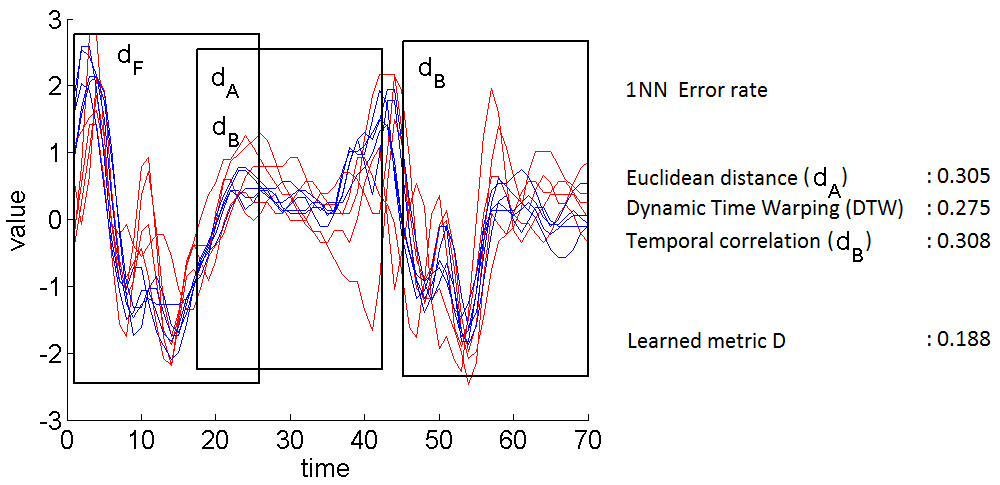
\includegraphics[width=0.8\linewidth]{SonyAIBO3}
	\caption{SonyAIBO dataset and error rate using a $k$NN ($k=1$) with standard metrics (Euclidean distance, Dynamic Time Warping, temporal correlation) and a learned combined metric $D$. The figure shows the 4 major metrics involve in the combined metric $D$ and their respective temporal scale (black rectangles).}
	\label{fig:SonyAIBO}
\end{figure}

% Ideally, a combined metric should answer two scenarios depending on the datasets: 1) combines several modalities at several scales; 2) select one modality at one particular scale and thus, coming back to a uni-modal and uni-scale metric framework. Figs. \ref{fig:SonyAIBO} and \ref{fig:ECG200} shows these two cases on two dataset examples used in classification of univariate time series. For SonyAIBO dataset (Fig. \ref{fig:SonyAIBO}), by learning the metric, several modalities (frequential $d_F$, behavior $d_B$ and amplitude $d_A$) at different locally temporal intervals are combined together. Thanks to this combination, the error of the 1-NN classifier is decreased: global uni-modal metrics achieves $0.305$ for $d_A$, $0.308$ for $d_B$, $0.258$ for $d_F$; and the combined metric achieves a score of 0.188. For ECG200 dataset (Fig. \ref{fig:ECG200}), the learned metric mainly includes the global behavior component $d_B$ and the error rate remains statistically the same. More detailed explanations will be given in Chapter \ref{sec:unchapitre}.

%\begin{table}[h!]
%	\small
%	\centering
%	\renewcommand{\arraystretch}{1}
%	\resizebox{0.75\textwidth}{!}{
%		\setlength{\tabcolsep}{1pt}
%		\begin{tabular}{|l|ccccc|ccc|}
%			\hline
%			& \multicolumn{5}{c|}{uni-modal metrics} & \multicolumn{2}{c}{Learned combined metrics} &  \\
%			\cline{2-9} 
%			Dataset & $d_A$ & $d_B$ & $d_F$ & $\mbox{\sc dtw}$ & $d_{B-\mbox{\sc dtw}}$ & $D$ & $D_{\mathcal{H}}$ & {\sc warp} \\
%			\hline
%			SonyAIBO            & 0.305 & 0.308 & 0.258 & 0.275 & 0.343     & \textbf{0.188} & \textbf{0.165} & $\times$   \\			
%			ECG200              & \textbf{0.120} & \textbf{0.070}& 0.160 & 0.230& 0.190    & \textbf{0.080} & \textbf{0.080} & $\times$  \\
%			\hline
%		\end{tabular}
%	}
%	\caption{1-NN  error rates for uni-modal metrics and learned combined metrics. Best equivalent performances for each dataset is indicated in bold. The considered metrics are respectively the Euclidean distance ($d_A$), the temporal correlation ($d_B$), the frequential-based distance ($d_F$), the dynamic time warping ({\sc dtw}), the temporal correlation computed on the signals re-align by the dynamic time warping ($d_{B-\mbox{\sc dtw}}$), a linear learned combined metric ($D$), a non-linear learned combined metric ($D_{\mathcal{H}}$). Last column ({\sc warp}) indicates if the learned combined metrics $D$ and $D_{\mathcal{H}}$ are computed with (\checkmark) or without warping ($\times$) }
%	\label{tab-resu2}
%\end{table}

%\begin{figure}[h!]
%\centering
%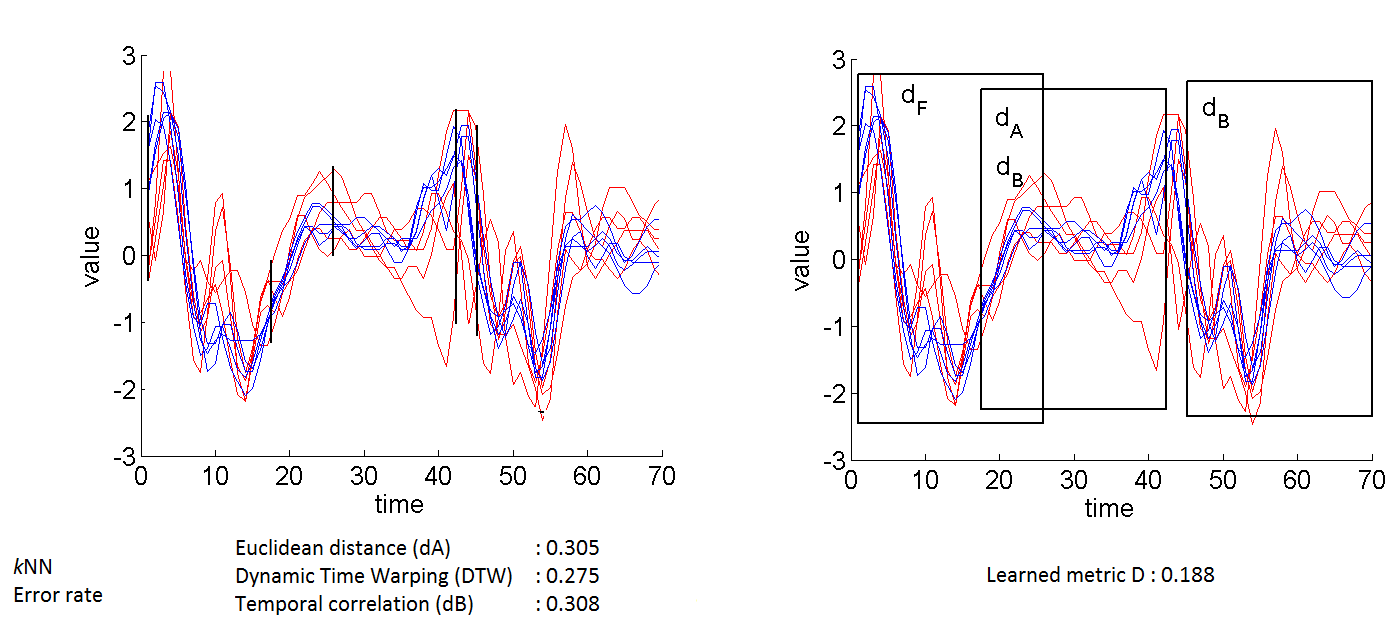
\includegraphics[width=1\linewidth]{images/SonyAIBO2}
%\caption{SonyAIBO dataset and error rate using a $k$NN with $k=1$ with standard metrics (Euclidean distance, Dynamic Time Warping, temporal correlation) (left) and a learned combined metric (right). For the learned combined metric $D$, the figure shows the 4 major metrics involves in the combination and their temporal scale (black rectangles).}
%\label{fig:SonyAIBO}
%\end{figure}
%
%
%\begin{figure}[h!]
%\centering
%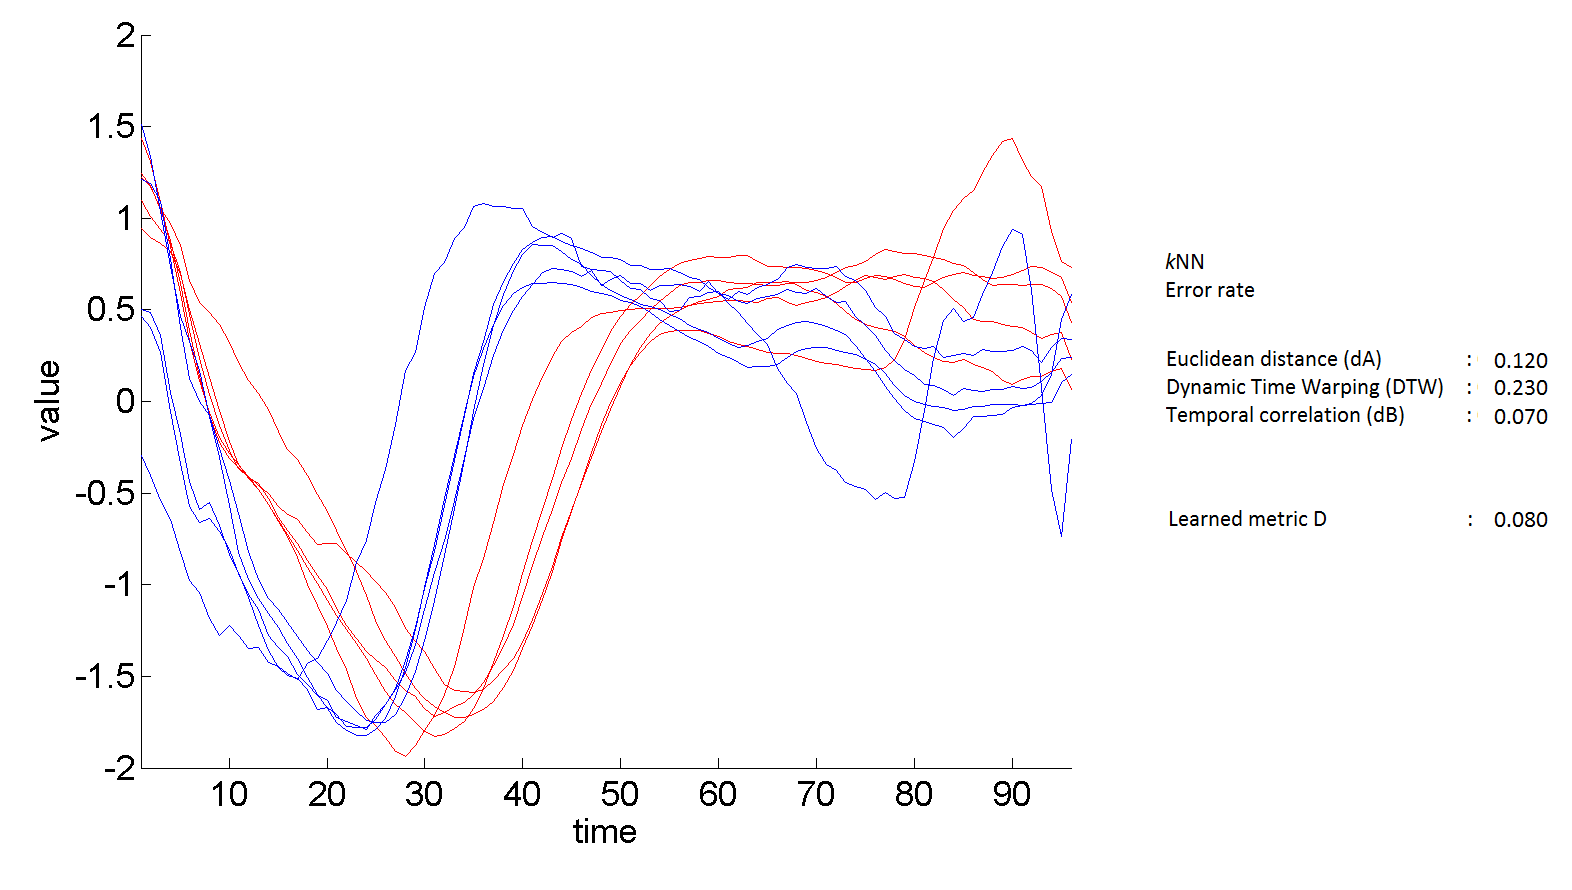
\includegraphics[width=0.7\linewidth]{images/ECG2002}
%\caption{ECG200 dataset and error rate using a $k$NN with $k=1$ with standard metrics (Euclidean distance, Dynamic Time Warping, temporal correlation) and a learned combined metric. For the learned combined metric $D$, the major discriminant feature is the behavior-based metric $d_B$ ($90\%$ of $D$) computed on a global scale (including all time series elements).}
%\label{fig:ECG200}
%\end{figure}




% \textcolor{blue}{The definition of a metric to compare samples is a fundamental issue in data analysis, pattern recognition or machine learning. For time series comparison, plenty of measures exist, most of them are designed to capture similitudes and differences based on one temporal modality, viz. by comparing time series based on their amplitudes, behaviors or frequential spectrum. For amplitude-based comparison, measures cover variants of Mahalanobis distance or the dynamic time warping to cope with delays [1, 2, 3, 4]. Other propositions refer to temporal correlations or derivative dynamic time warping for behavior-based comparison [5, 6, 7, 8, 9]. For frequential aspects, comparisons are mostly based on the Discret Fourier or Wavelet Transforms [10, 11, 12, 13]. A detailed review of the major metrics is proposed in [14]. \\
 %More recent works enhance the potential of temporal metrics by combining several modalities through a priori models as in [15, 16, 17]. For all these temporal measures, there is still room for improvement to handle complex time series by: a) integrating several modalities through a learned linear or non linear models, instead of a priori ad-hoc ones and b) involving totally or partially time series elements, rather than systematically the whole elements as operated for the most, if not all, available temporal measures.} \\


% \noindent \textbf{Motivation du Metric Learning}
%\begin{itemize}
%	\item Commencer par le metric learning en général: definition
%	\item Metric learning a eu de nombreux attraits ces dernières années, que ce soit pour les features data et les structures data (tree, graph, strings). De nombreux surveys ont été fait (Yan \& Jin, Kulis, Bellet \& al.). Elle a reçu de nombreuses recherches actives: preuves théoriques (generalization guarantees) et couvert les différents problèmes du machine learning (supervised, semi-supervised et non supervisé, online learning).
%	\item for feature data (static data) a reçu de nombreuses recherches principalement divisable en 2 catégories : linéaire et non linéaire (inspiré des SVMs, adaptation des algos ou combinaison avec des SVM). Très souvent, le problème revient à apprendre une matrice de Mahalanobis. L'approche la plus populaire qui a reçu de nombreuses extensions est celle proposée par Weinberger : LMNN.
%	\item focaliser sur le metric learning pour les données structurées : moins nombreuses et a reçu moins d'attention. Elle repose souvent sur l'optimisation de l'Edit distance
%	\item Les séries temporelles pouvant être vu comme des données structurées, les recherches dans le domaine du metric learning sont encore moins nombreuses (reprendre PRL)
%	\item terminer sur la remarque du papier de Bellet : learning richer metrics : multi-modalité
%	\item mettre les + et - de chaque méthode.
%	\item S'appuyer sur le papier de Aurélien Bellet
%\end{itemize}

\todo{Correction d'anglais et précision des phrases} Our aim is to take leverage from the metric learning framework \cite{Weinberger2009a,Bellet2012} to learn a multi-modal and multi-scale temporal metric for time series nearest neighbors classification. Specifically, our objective is to learn from the data a linear or non linear function that combines several temporal modalities at several temporal scales, that satisfies metric properties (Section \ref{sec:property_metric}), and that generalizes the case of unimodal metrics at the global scale. \\
Metric learning can be defined as learning, from the data and for a task, a pairwise function (\textit{i.e.} a similarity, dissimilarity or a distance) that brings closer samples that are expected to be similar, and pushes \todo{separate} far away those expected to be dissimilar. Such similarity and dissimilarity expectations, is inherently task- and application-dependent, generally given \textit{a priori} and fixed during the learning process. Metric learning has become an active area of research in the last decade for various machine learning problems (supervised, semi-supervised, unsupervised, online learning) and has received many interests in its theoretical background (generalization guarantees) \cite{Bellet2013a}. From the surge of recent research in metric learning, one can identify mainly two categories: the linear and non linear approaches. The former is the most popular, it defines the majority of the propositions, and focuses mainly on the Mahalanobis distance learning \cite{Weinberger2009}. The latter addresses non linear metric learning which aims at capturing non linear structure in the data, \textit{e.g.}, Kernel Principal Component Analysis (KPCA) and Support Vector Metric Learning (SVML). In both cases, the metric is directly learned in the original space (\textit{i.e.}, space described by the features of the samples).\mycomment[SMA]{Appuyer différence} In KPCA, the aim is to project the data into a non linear feature space and learn the metric in that projected space \cite{Zhang2010,Chatpatanasiri2010}. In SVML, the Mahalanobis distance is learned jointly with the learning of the SVM model in order to minimize the validation error \cite{Xu2012}. In general, the optimization problems in non linear approaches is more expensive to solve that in linear approaches, and the methods tends to favor overfitting as the constraints are generally easier to satisfy in a nonlinear kernel space. A more detailed review on metric learning is done in \cite{Bellet2013a}.\\
Contrary to static data, metric learning for structured data (\textit{e.g.} sequence, time series, trees, graphs, strings) is less frequent. While for sequence data most of the works focus on string edit distance to learn the edit cost matrix \cite{Oncina2006,Bellet2012}, metric learning for time series is still in its infancy. Without being exhaustive, major recent proposals rely on weighted variants of dynamic time warping to learn alignments under phase or amplitude constraints \cite{Reyes2011,Jeong2011,ZhangX.-L.Z.-G.Luo2014}, enlarging alignment learning framework to multiple temporal matching guided by both global and local discriminative features \cite{Frambourg2013a}. For most of these propositions, temporal metric learning process is systematically: a) Uni-modal (amplitude-based), the divergence between aligned elements being either the Euclidean or the Mahalanobis distance and b) Uni-scale (global level), involving all time series elements at once, which restricts its potential to capture local characteristics. We believe that perpectives for metric learning, in the case of time series, should include multi-modal and multi-scale aspects.

We propose in this work to learn a multi-modal and multi-scale temporal metric for a robust $k$-NN classifier. For this, the main idea is to embed time series into a pairwise dissimilarity space\mycomment[MR]{ajouter pairwise pour différencier} where a linear function combining several modalities at different temporal scales can be learned, driven by a large margin optimization process inspired from the nearest neighbors metric learning framework \cite{Weinberger2009a} \mycomment[SMA]{modif pour dire que le processus est général et pas que SVM}. Thanks to the "kernel trick", the proposed solution is extended to non-linear temporal metric learning context. A sparse and interpretable variant of the proposed metrics confirms its ability to localize finely discriminative modalities as well as their temporal scales. In the following, the term metric is used to reference both a distance or a dissimilarity measure.

In this chapter, we first present the concept of pairwise dissimilarity space. Then, we formalize the general problem of learning a combined metric for a robust $k$-NN as the learning a function in the dissimilarity space. From the general formalization, we propose three formalizations (Linear, Quadratic and \textsc{svm}-based), give an interpretation of the solutions and study the properties of the learned metrics. Finally, we give the algorithm. Note that these formalizations don't concern only time series and can be applied to learn a combined metric on any type of data. \todo{Mettre la section LMNN ici?}


%---------------------------------------------------------------------------
\section{Multi-modal and multi-scale dissimilarity space} \todo{titre à changer?}
%\section{Pairwise dissimilarity space} 
\label{sec:Pairwise_embedding}
%\begin{itemize}
%	\item Changement de l'espace
%	\item Normalisation de l'espace des paires
%	\item Label des pairwise
%\end{itemize}
\todo{ref: dissimilarity space \cite{Pcekalska2002,Duin2012}}
In this section, we first present the concept of dissimilarity space for multi-modal metrics. Then, in the case of time series, we enrich this representation with a multi-scale description. 

\subsection{Pairwise embedding}
Let $\{\textbf{x}_{i}, y_{i}\}_{i=1}^n$ be a set of $n$ time series $\textbf{x}_i = [x_{i1}, \ldots, x_{iq}] \in \mathbb{R}^q$ labeled $y_{i}$ \mycomment[SMA]{label maintenant?}. Let  $d_1, \ldots , d_p$ be $p$ given metrics that allow to compare samples $\textbf{x}_{i}$. As discussed in Chapter \ref{sec:Chapter_metrics}, three naturally modalities are involved for time series comparison: amplitude-based $d_A$, behavior-based $d_B$ and frequential-based $d_F$. Our objective is to learn a metric $D$ that combines the $p$ basic temporal metrics for a robust $k$-NN classifier.

The computation of a metric $d$, and $D$, always takes into account a pair of samples $(\textbf{x}_i,\textbf{x}_j)$. We introduce a new space representation referred as the \textbf{dissimilarity space}. We note $\varphi$ an embedding function that maps each pair of time
series $(\textbf{x}_i, \textbf{x}_j)$ to a vector $\textbf{x}_{ij}$ in a dissimilarity space $\mathcal{E} = \mathbb{R}^p$ whose dimensions are $d_1, \ldots, d_p$ (Fig. \ref{fig:PairwiseEmbedding}):
\begin{equation}
\begin{aligned}
\varphi : \mathbb{R}^q \times \mathbb{R}^q & \rightarrow \mathcal{E} = \mathbb{R}^p \\
(\textbf{x}_i, \textbf{x}_j) & \rightarrow \textbf{x}_{ij} = [d_1(\textbf{x}_i, \textbf{x}_j), \ldots, d_p(\textbf{x}_i, \textbf{x}_j)]^T
\end{aligned}
\label{eq:projection}
\end{equation}

\begin{figure}[h!]
	\begin{minipage}[b]{1.0\linewidth}
		\centering
		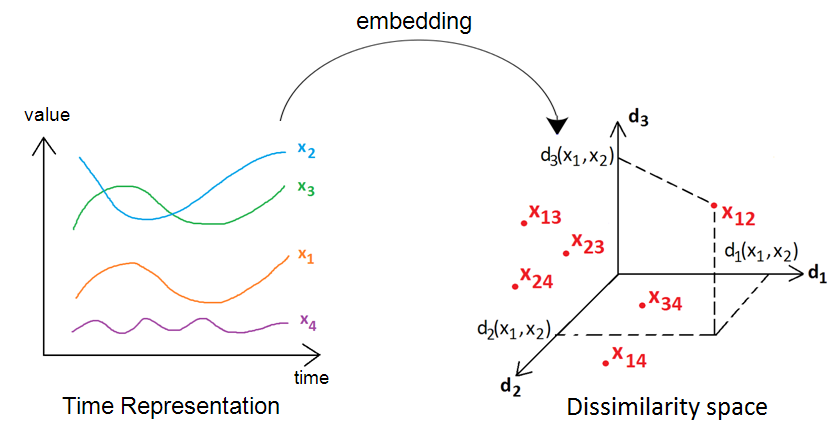
\includegraphics[width=0.85\linewidth]{images/PairwiseEmbedding2}
	\end{minipage}
	\caption{Example of embedding of time series $\textbf{x}_i$ from the temporal space (left) into the dissimilarity space (right) for $p=3$ basic metrics.}
	\label{fig:PairwiseEmbedding}
\end{figure}

\noindent A metric $D$ that combines the $p$ metrics $d_1, \ldots, d_p$ can be seen as a function of the dissimilarity space: \mycomment[SMA]{Proposition pour mettre en valeur que c'est une fonction}
\begin{equation}
\begin{aligned}
D : \mathbb{R}^p & \rightarrow \mathbb{R} \\
\textbf{x}_{ij} & \rightarrow D(\textbf{x}_{ij}) = f(d_1(\textbf{x}_i, \textbf{x}_j), \ldots , d_p(\textbf{x}_i, \textbf{x}_j))
\end{aligned}
\label{eq:metric}
\end{equation}
In that space, the norm of a pairwise vector $||\textbf{x}_{ij}||$ refers to the proximity between the time series $\textbf{x}_i$ and $\textbf{x}_j$. In particular, if $||\textbf{x}_{ij}||=0$ then $\textbf{x}_j$ is identical to $\textbf{x}_i$ according to all metrics $d_h$. Note that in this space, the proximity between pairs can't be interpreted.

\subsection{Multi-scale description for time series} \mycomment[SMA]{Basculer en chap 2?}
As illustrated in Fig. \ref{fig:SonyAIBO}, the multi-modal representation in the dissimilarity space can be enriched for time series by measuring each unimodal metric $d_h$ at different scales. Note that the distance measures (amplitude-based $d_A$, frequential-based $d_F$, behavior-based $d_B$) in Eqs. \ref{eq:A}, \ref{eq:F} and \ref{eq:B} implies systematically the total time series elements $x_{it}$ and thus, restricts the distance measures to capture local temporal differences. In our work, we provide a multi-scale framework for time series comparison using a hierarchical structure. Many methods exist in the literature such as the sliding window or the dichotomy \todo{ref}. We detail here the latter one. \\
\indent A multi-scale description can be obtained by repeatedly segmenting a time series expressed at a given temporal scale to induce its description at a more local level. Many approaches have been proposed assuming fixed either the number of the segments or their lengths. In our work, we consider a binary segmentation at each level. Let $I=[a;b]$ be a temporal interval of size $(b-a)$. The interval $I$ is decomposed into two equal overlapped intervals $I_L$ (left interval) and $I_R$ (right interval). A parameter $\alpha$ allows to overlap the two intervals $I_L$ and $I_R$, covering discriminating subsequences in the central region of $I$ (around $\frac{b+a}{2}$): $I = [a;b]; I_L = [a;a+\alpha(b-a)]; I_R = [b-\alpha(b-a);b]$. 
%\begin{align}
%	I &= [a;b] \\
%	I_L &= [a;a+\alpha(b-a)] \\
%	I_R &= [a-\alpha(b-a);b] 
%	\label{key}
%\end{align}
\noindent For $\alpha = 0.6$, the overlap covers $10\%$ of the size of the interval $I$. Then, the process is repeated on the intervals $I_L$ and $I_R$. We obtain a set of intervals $I_s$ illustrated in Fig. \ref{fig:Intervalles}. \\
A multi-scale dissimilarity description between two samples is obtained by computing the usual time series metrics ($d_A$, $d_B$, $d_F$) on each of the resulting segments $I_s$. Note that for two time series $\textbf{x}_i$ and $\textbf{x}_j$, the comparison between $\textbf{x}_i$ and $\textbf{x}_j$ is done on the same interval $I_s$. For a multi-scale amplitude-based comparison based on binary segmentation, the set of involved amplitude-based measures $d^{Is}_A$ is $\{d^{I_1}_A, d^{I_2}_A, \ldots \}$ where $d^{Is}_A$ is defined as:
\begin{equation}	
d^{Is}_A(\textbf{x}_i,\textbf{x}_j) = \sqrt{\sum\limits_{t \in Is} (x_{it}-x_{jt})^2}
\label{eq:A2}
\end{equation}
The local behaviors- and frequential- based measures $d^{Is}_B$ and $d^{Is}_F$ are obtained similarly.
\begin{figure}[h!]
	\centering
	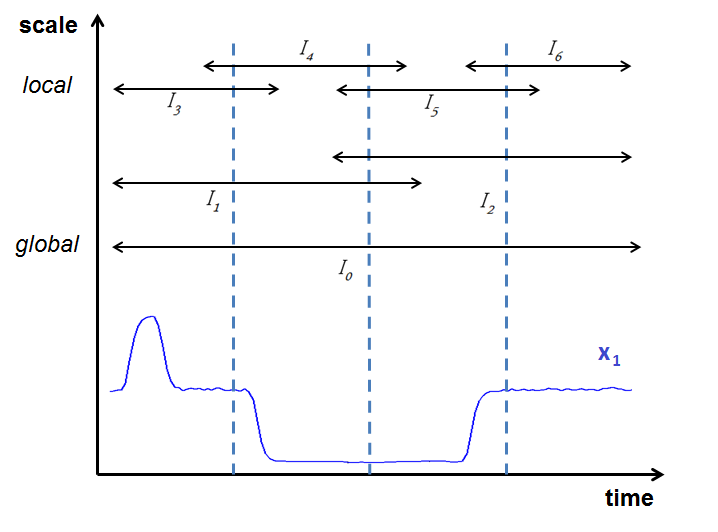
\includegraphics[width=0.5\linewidth]{images/Intervalles3}
	\caption{Multi-scale decomposition}
	\label{fig:Intervalles}
\end{figure}

\noindent In the following, for simplification purpose, we consider $d_1, \ldots, d_p$ as the set of multi-modal and multi-scale metrics.

\subsection{Interpretation in the dissimilarity space}
%\begin{itemize}
%	\item Proximity to the origin (les individus sont identiques)
%	\item Proximity of 2 pairwise points in the pairwise space 
%	\item Norm in the pairwise space
%	\item Representation of combined metric in the pairwise space
%	\item perte de la classe initiale des individus. L'information qui nous reste est : les 2 individus sont de la même classe ou sont de classes différentes.
%\end{itemize}

In this section, we give more detailed interpretations in the dissimilarity space. \todo{Sous section ajoutée, ok pour SMA et MR}
We recall that the norm of a pairwise vector is given by: 
\begin{equation}
||\textbf{x}_{ij}|| = \sum\limits_{h=1}^{p} d_h(\textbf{x}_{i},\textbf{x}_{j})
\end{equation}
In the following, we denote the norm as an initial distance in the dissimilarity space and call it $D_0$. The norm of a pairwise vector $\textbf{x}_{ij}$ can be interpreted as a proximity measure: the lower the norm of $\textbf{x}_{ij}$ is, the closer are the time series $\textbf{x}_{i}$ and $\textbf{x}_{j}$. Two pairwise vectors $\textbf{x}_{ij}$ and $\textbf{x}_{kl}$ that are on a same line that passes through the origin $\textbf{x}_{ii} = \textbf{0}$ represent differences in the the same proportions between their respective modalities (Fig. ??). 

\begin{figure}[h!]
	\centering
	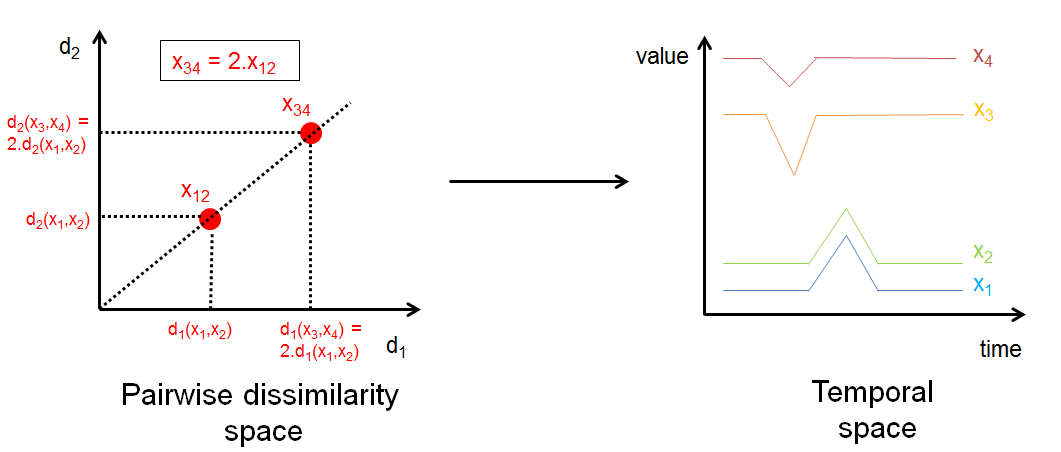
\includegraphics[width=1\linewidth]{Pairwise_interpretation}
	\caption{Example of two pairwise vectors $\textbf{x}_{12}$ and $\textbf{x}_{34}$ close in the pairwise space. However, the time series $\textbf{x}_{1}$ and $\textbf{x}_{3}$ are not similar in the temporal space.}
	\label{fig:pairwise_interpretation}
\end{figure}

The euclidean distance $\sqrt{\sum\limits_{h=1}^{p} (d_h(\textbf{x}_{i},\textbf{x}_{j})-d_h(\textbf{x}_{k},\textbf{x}_{l}))^2}$ between two pairwise vectors $\textbf{x}_{ij}$ and $\textbf{x}_{kl}$ represent the similarity between the differences among the same modality, in the same proportion. Note that if the euclidean distance is close to 0 ($\textbf{x}_{ij}$ and $\textbf{x}_{kl}$ are close in the dissimilarity space) it doesn't mean that the time series $\textbf{x}_{i}$, $\textbf{x}_{j}$, $\textbf{x}_{k}$ and $\textbf{x}_{l}$ are similar. Fig \ref{fig:ContreExample} shows an example of two pairwise vectors $\textbf{x}_{ij}$ and $\textbf{x}_{kl}$ close together in the pairwise space. However, in the temporal space, the time series $\textbf{x}_{1}$ and $\textbf{x}_{3}$ are not similar for example. It means that $\textbf{x}_i$ is as similar to $\textbf{x}_j$ as $\textbf{x}_k$ is to $\textbf{x}_l$, \textit{i.e.}, the distance $D_0$ between $\textbf{x}_i$ and $\textbf{x}_j$ is roughly the same than the distance $D_0$ between $\textbf{x}_k$ and $\textbf{x}_l$.

\begin{figure}[h!]
	\centering
	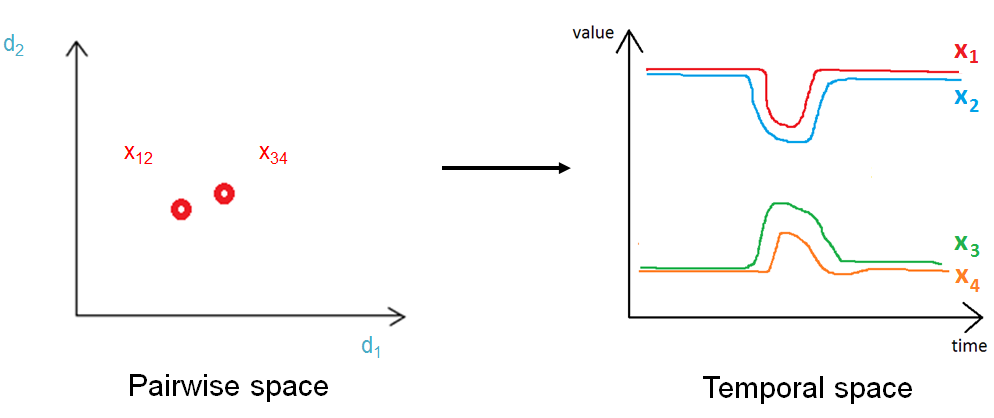
\includegraphics[width=0.85\linewidth]{ContreExample}
	\caption{Example of two pairwise vectors $\textbf{x}_{12}$ and $\textbf{x}_{34}$ close in the pairwise space. However, the time series $\textbf{x}_{1}$ and $\textbf{x}_{3}$ are not similar in the temporal space.}
	\label{fig:ContreExample}
\end{figure}

% A metric $D$ that combines the $p$ unimodal metrics $d_1, \ldots, d_p$ can be seen as a function of the pairwise space. It can be noticed that when the time series $\textbf{x}_i$ are embedded in the pairwise, the information of their original class $y_i$ is lost. Any multi-class problem is transformed in the pairwise space as a binary classification problem.



\section{M$^2$TML general problem}
In this section, we propose to define the Multimodal and Multiscale Time series Metric Learning ({\sc m$^2$tml}) problem in the initial space as a general problem of learning a function in the dissimilarity space. First, we give the intuition and formalize the general optimization problem. Secondly, we propose different strategies to define the neighborhood.

\subsection{General formalization for M$^2$TML} 
Our objective is to learn a dissimilarity $D=f(d_1, \ldots, d_p)$ in $\mathcal{E}$, the embedding space, that combines the $p$ dissimilarities $d_1, \ldots, d_p$ for a robust $k$-NN classifier. The function $f$ can be linear or non-linear and must satisfy at least the properties of a dissimilarity, \textit{i.e.}, positivity ($D(\textbf{x}_{ij} \geq 0)$), reflexivity ($D(\textbf{x}_{ii})=0 \text{ }\forall i$) and symmetry ($D(\textbf{x}_{ij}) = D(\textbf{x}_{ji}) \text{ } \forall i,j$) (Section \ref{sec:property_metric}). To simplify the discussion in the following, we refer to dissimilarity as metrics. The proposition is based on two standard intuitions in metric learning, \textit{i.e.}, for each time series $\textbf{x}_i$, the metric $D$ should bring closer the time series $\textbf{x}_j$ of the same class ($y_j=y_i$) while pushing the time series $\textbf{x}_l$ of different classes ($y_l \neq y_i$). These two sets are called respectively $Pull_i$ and $Push_i$. 
% Fig. \ref{fig:Transposition_Pairwise2} illustrates that concept.
\todo{figure enlevée ici car trop tôt}Formally, the metric learning problem can be written as an optimization problem that involves both a regularizion term $R(Pull)$\mycomment[SMA]{mettre $R(D,Pull)$?} and a loss term $L(Push)$ under constraints that controls the push term:

\begin{equation}
\begin{aligned}
&\displaystyle 		\argmin_{D,\xi} \left[  R(Pull) + L(Push) \right] \\
&\text{s.t. \textit{constraints} }
\end{aligned}
\end{equation}

\noindent The problem of learning a combined metric $D$ for large margin $k$-NN classification can be written as the following optimization problem:

\begin{equation}
\begin{aligned}
&\displaystyle 		\argmin_{D,\xi} \left\lbrace \underbrace{
	\vphantom{ \sum\limits_{\substack{i \\ j \in Pull_i \\ l \in Push_i}} \frac{1-y_{il}}{2} \xi_{ijl} }
	\sum_{\substack{i \\ j \in Pull_i}}D(\textbf{x}_{ij})
}_{pull}
+ C
\underbrace{
	\sum\limits_{\substack{i \\ j \in Pull_i \\ l \in Push_i}} \frac{1-y_{il}}{2} \xi_{ijl}
}
_{push} \right\rbrace  \\
&\text{s.t.  } \forall i = 1, \ldots, n, \forall j \in Pull_i, l \in Push_i, \\
& \qquad D(\textbf{x}_{il})-D(\textbf{x}_{ij}) \geq 1-\xi_{ijl} \\
& \qquad \xi_{ijl} \geq 0 
\label{eq:OriginalOptimizationProblem_Objective} 
\end{aligned}
\end{equation}
\noindent where $y_{il} = -1$ if $y_i \neq y_l$ and +1 otherwise, \mycomment[SMA]{Enlever les $y_{il}$, ils ne servent plus}$\xi_{ijl}$ are the slack variables and $C$, the trade-off between the pull and push costs. In the next section, we detailed different strategies to define the $Pull_i$ and $Push_i$ sets. 

%\begin{figure}[t]
%	\centering
%	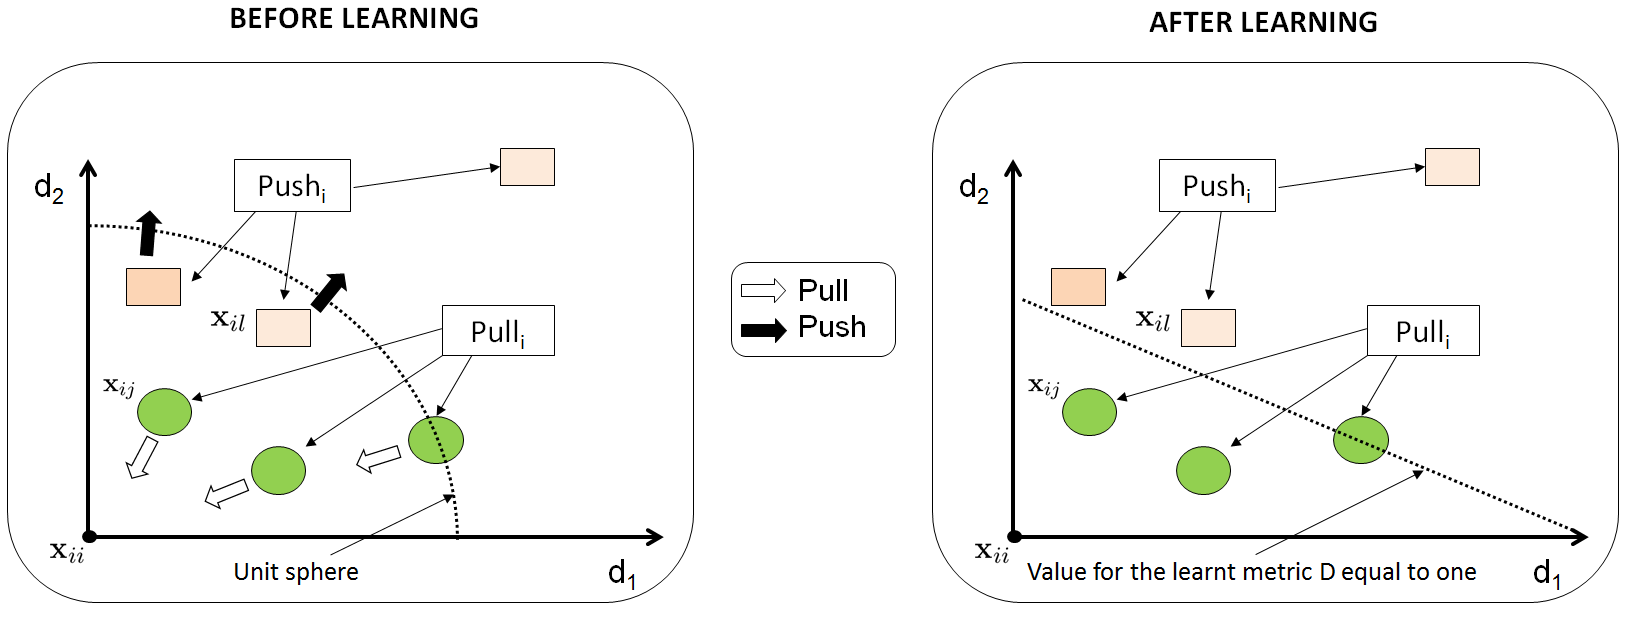
\includegraphics[width=1\linewidth]{images/Transposition_Pairwise3}
%	\caption{Geometric representation of the metric learning problem in the dissimilarity space for a $k=3$ target neighborhood of $\textbf{x}_i$. Before learning (left), push samples $\textbf{x}_l$ invade the targets perimeter $\textbf{x}_j$. In the dissimilarity space, this is equivalent to have pairwise vectors $\textbf{x}_{il} \in Push_i$ with a norm lower to some pairwise target $\textbf{x}_{ij} \in Pull_i$. The aim of metric learning is to push pairwise $\textbf{x}_{il}$ (black arrow) and pull pairwise $\textbf{x}_{ij}$ from the origin (white arrow).}
%	\label{fig:Transposition_Pairwise2}
%\end{figure}

\subsection{Push and pull set definition}
To build the pairwise training set, we associate for each $\textbf{x}_i$, two sets, $Pull_i$ and $Push_i$, where the two sets are chosen according to one of the following strategies, illustrated in Fig \ref{fig:Strategy_neighborhood}: \todo{Ajouter une remarque sur $D_0$?}
\begin{enumerate}
	\item \textbf{$k$-NN vs impostors}: for a given $\textbf{x}_i$, the sets of pairs to pull and to push corresponds respectively to:
	\begin{align}
		\forall i\in 1, \ldots, n, \quad Pull_i & = \{\textbf{x}_{ij} \text{ } / \text{ }  \text{$y_j = y_i$, $||\textbf{x}_{ij}||_2$ is among the $k$-lowest norms} \} \label{eq:pull1}\\
		Push_i & = \{\textbf{x}_{il} \text{ } / \text{ } \text{$y_l \neq y_i$, } ||\textbf{x}_{il}||_2 \leq \max\limits_{\textbf{x}_{ij} \in Pull_i} ||\textbf{x}_{ij}||_2\} \label{eq:push1}
	\end{align}
	\item \textbf{$k$-NN vs all}: for a given $\textbf{x}_i$, the sets of pairs to pull and to push corresponds respectively to:	
	\begin{align}
	\forall i\in 1, \ldots, n, \quad Pull_i & = \{\textbf{x}_{ij} \text{ } / \text{ } \text{$y_j = y_i$, $||\textbf{x}_{ij}||_2$ is among the $k$-lowest norms} \} \\
	Push_i & = \{\textbf{x}_{il} \text{ } / \text{ } \text{$y_l \neq y_i$} \}
	\end{align}
	\item \textbf{$m$-NN$^+$ vs $m$-NN$^-$}: for a given $\textbf{x}_i$, the pull and push sets are defined respectively as 
	the set of the $m$-nearest neighbors of the same class ($y_j=y_i$), 
	and the $m$-nearest neighbor of $\textbf{x}_i$ of a different class ($y_j \neq y_i$)
	More precisely, our proposition states: $m=\alpha.k$ with $\alpha \geq 1$. Other propositions for $m$ are possible:
	\begin{align}
	\forall i\in 1, \ldots, n, \quad Pull_i & = \{\textbf{x}_{ij} \text{ } / \text{ } \text{$y_j = y_i$, $||\textbf{x}_{ij}||_2$ is among the $m$-lowest norms} \} \label{eq:mnn+}\\
	Push_i & = \{\textbf{x}_{il} \text{ } / \text{ } \text{s.t. $y_l \neq y_i$, $||\textbf{x}_{il}||_2$ is among the $m$-lowest norms} \} \label{eq:mnn-}
	\end{align}
	In the following, we denote $m\text{-NN}^+ = \bigcup\limits_{i} Pull_i$ and $m\text{-NN}^- = \bigcup\limits_{i} Push_i$
\end{enumerate}
\begin{figure}[h!]
	\centering
	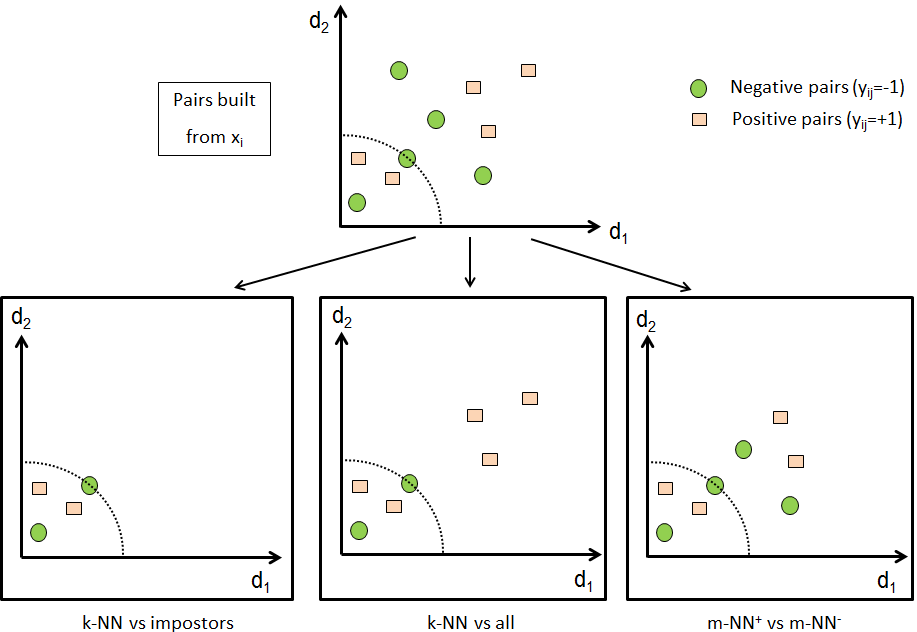
\includegraphics[width=0.9\linewidth]{images/Strategy_neighborhood}
	\caption{Example of different strategies to build $Pull_i$ and $Push_i$ sets for a $k=2$ neighborhood.}
	\label{fig:Strategy_neighborhood}
\end{figure}

Finally, let discuss about the similarities and differences between \textsc{lmnn} (Weinberger \& Saul~\cite{Weinberger2009}) and our \textsc{m$^2$tml} proposition. In \textsc{lmnn}, the sets $Pull_i$ and $Push_i$ are defined according the \textbf{$k$-NN vs impostors} strategy (Eqs. \ref{eq:pull1} \& \ref{eq:push1}) and may be unbalanced. The sets are defined and fixed during the optimization process according to an initial metric (Euclidean distance). In \textsc{m$^2$tml} the sets $Pull_i$ and $Push_i$ are defined according the \textbf{$k$-NN vs impostors} strategy (Eqs. \ref{eq:mnn+} \& \ref{eq:mnn-}) and are balanced. The sets are defined and fixed during the optimization process according to an initial metric (Euclidean distance), but the $m$-neighborhood is larger than the $k$-neighborhood. By considering a neighborhood larger than the $k$-neighborhood (\textbf{$k$-NN vs impostors} strategy), we believe that the generalization properties of the learnt metric $D$ would be improved. 

%\noindent Even if the optimization problem in Eq. \ref{eq:OriginalOptimizationProblem_Objective} is similar to the one of Large Margin Nearest Neighbors ({\sc lmnn}) proposed by Weinberger \& Saul in ~\cite{Weinberger2009} (Eq. \ref{eq:OptimizationProblem}), let recall the main points:
%\begin{itemize}
%	\item The sets $Pull_i$ and $Push_i$ are defined according the \textbf{$k$-NN vs impostors} strategy.
%	\item The sets $Pull_i$ and $Push_i$ can be unbalanced.
%	\item The initial distance is the Euclidean distance.
%	\item The sets $Pull_i$ and $Push_i$ are defined and fixed during the optimization process according to the considered initial metric.
%	\item The learnt metric $D$ is a Mahalanobis distance.
%\end{itemize}
%
%\noindent Our proposition ({\sc m$^2$tml}) differs from {\sc lmnn} and we detailed here the main points:
%\begin{itemize}
%	\item The sets $Pull_i$ and $Push_i$ are defined according the \textbf{$m$-NN$^+$ vs $m$-NN$^-$} strategy with $m=\alpha.k$, $\alpha \geq 1$.
%	\item The sets $Pull_i$ and $Push_i$ are balanced.
%	\item The initial distance is the Euclidean distance.
%	\item The sets $Pull_i$ and $Push_i$ are defined and fixed during the optimization process according to the considered initial metric. However, the $m$-neighborhood is larger than the $k$-neighborhood allowing a better generalization of the learnt metric $D$.
%	\item The learnt metric $D$ is a combined metric of several unimodal metrics measured at different scales.
%\end{itemize}

\subsection{Interpretation in the dissimilarity space}
In this section, we give more detailed interpretations of the \textsc{m$^2$tml} problem in the dissimilarity space. \todo{Ajout ok pour SMA et MR}Our objective is to learn a metric $D$ as a linear or non-linear combination of the $p$ unimodal metrics $d_1, \ldots, d_p$. The metric $D$ can be seen as a function of the dissimilarity space that should:
\begin{itemize}
	\item \textbf{pull} to the origin $\textbf{x}_{ii} = \textbf{0}$ the pairs $\textbf{x}_{ij}$ of $Pull_i$
	\item \textbf{push} away from the origin all the pairs $\textbf{x}_{il}$ of $Push_i$
\end{itemize}
Fig. \ref{fig:Transposition_Pairwise} illustrates the idea in the original space and in the dissimilarity space: first, we build the sets $Pull_i$ and $Push_i$ according to an initial metric $D_0$; secondly, we optimize the metric $D$ so that the pairs $Pull_i$ are pulled to the origin and the pairs $Push_i$ are pushed away from the origin.

\begin{figure}[t!]
	\centering
	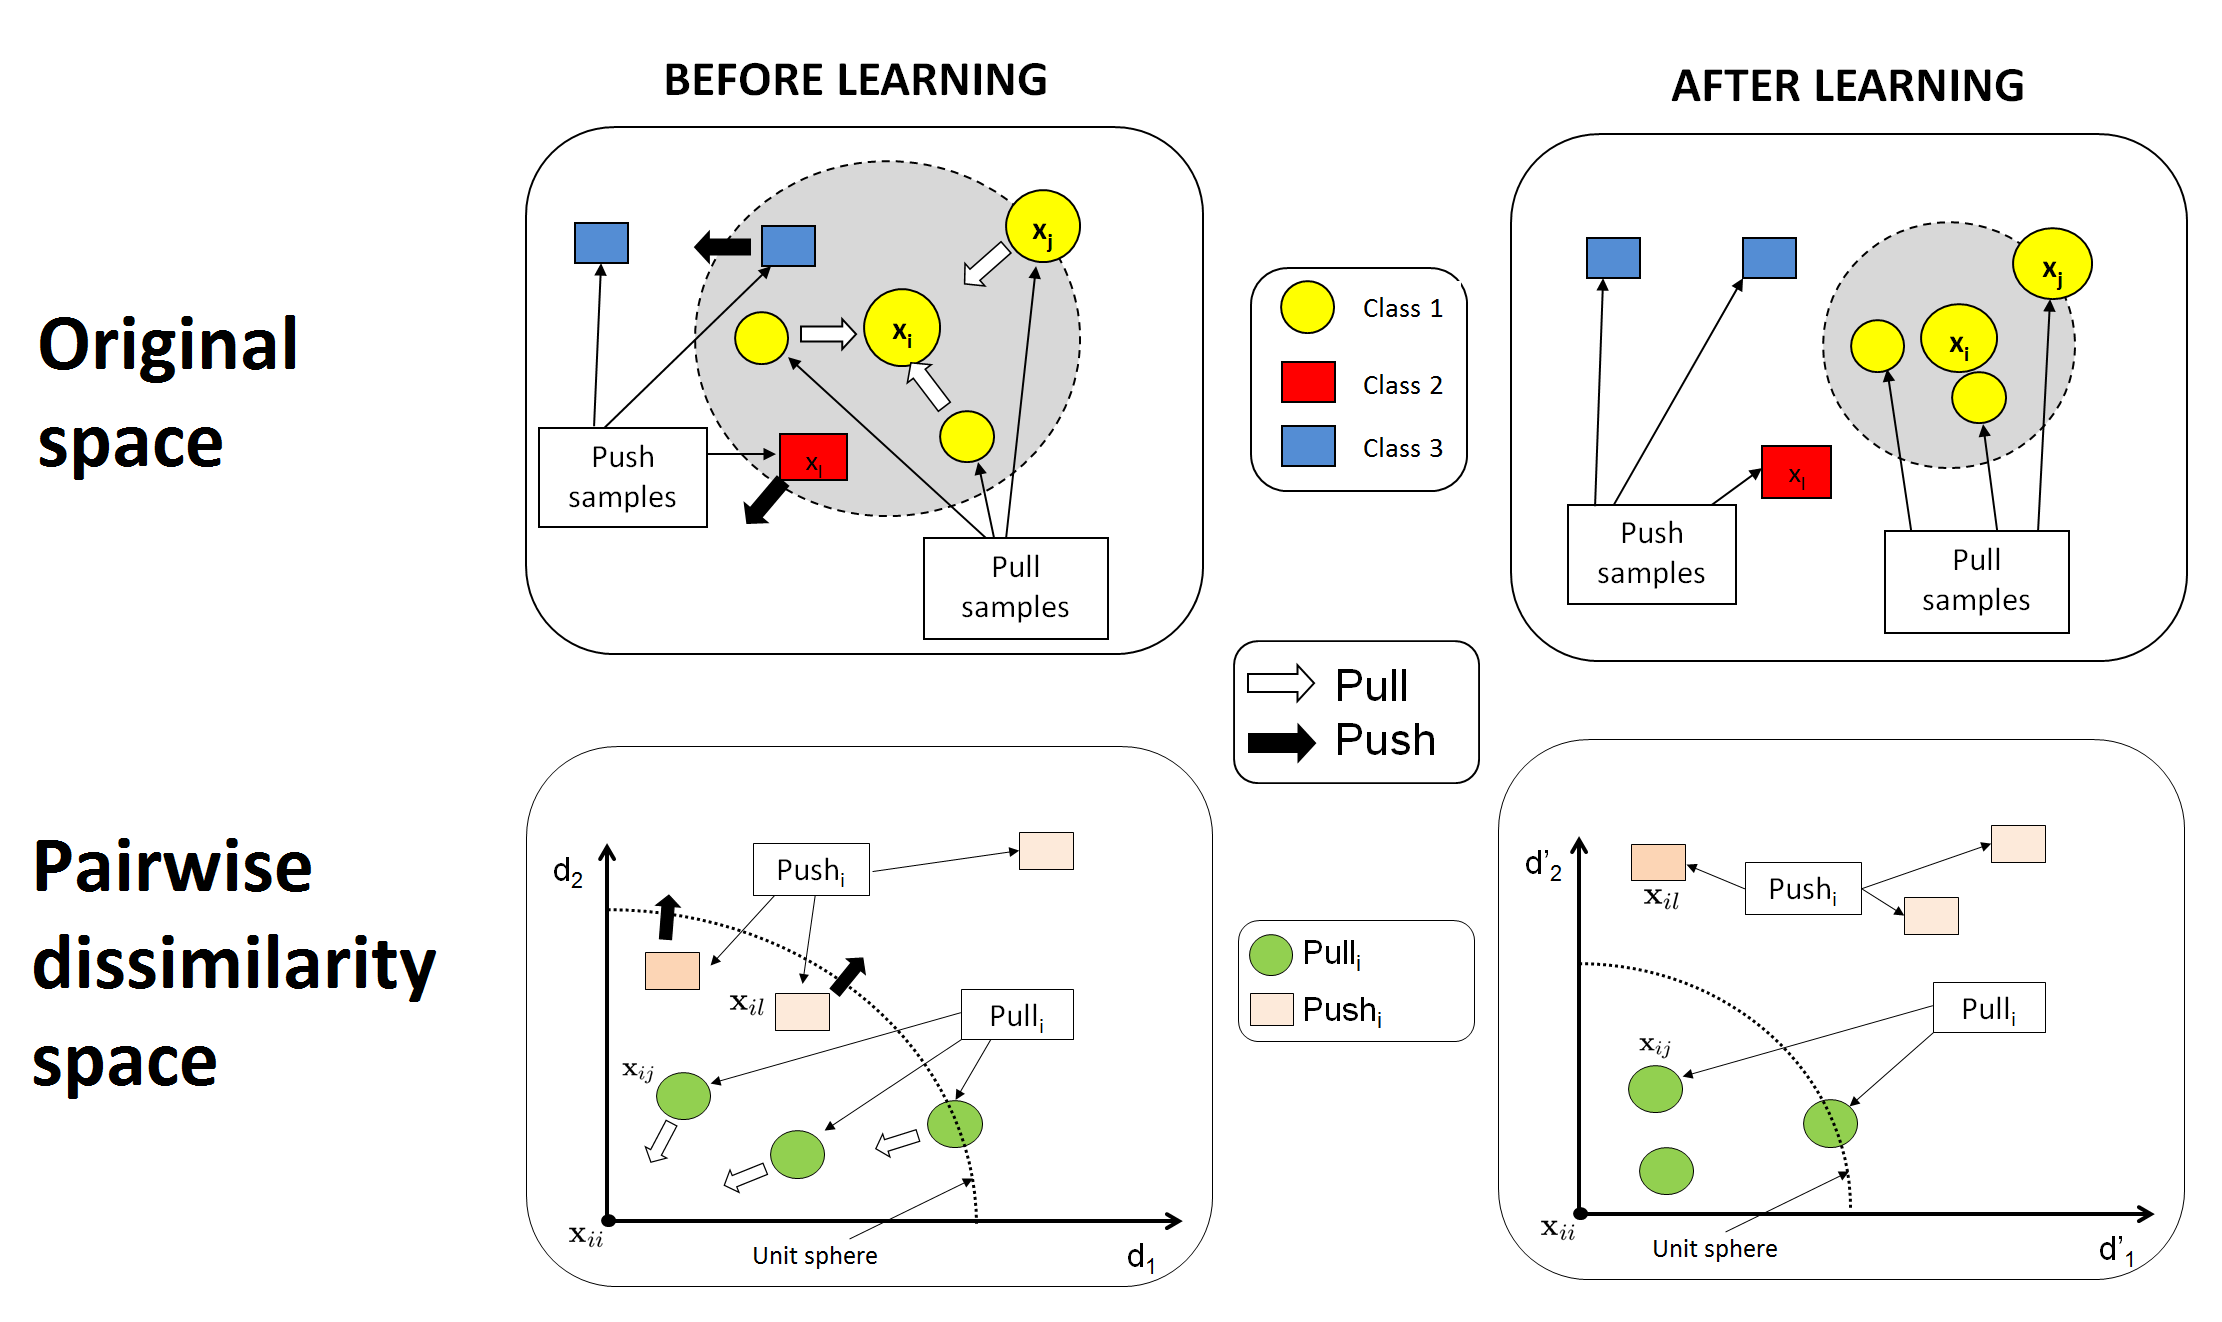
\includegraphics[width=1\linewidth]{Transposition_Pairwise4}
	\caption{Metric learning problem from the original space (top) to the dissimilarity space (bottom) for a $k=3$ neighborhood of $\textbf{x}_i$. Before learning (left), push samples $\textbf{x}_l$ invade the targets perimeter $\textbf{x}_j$. In the pairwise space, this is equivalent to have push pairwise vectors $\textbf{x}_{il}$ with an initial distance $D_0$ lower than the distance of pull pairwise vectors $\textbf{x}_{ij}$. The aim of metric learning is to learn a metric $D$ to push $\textbf{x}_{il}$ (black arrow) and pull $\textbf{x}_{ij}$ from the origin (white arrow).}
	\label{fig:Transposition_Pairwise}
\end{figure}
\noindent Note that by considering a larger neighborhood, we ensure that pairs $Push_i$ doesn't invade the perimeter defined by pairs $Pull_i$. Similarly to the interpretation of slack variables in \textsc{svm}, if a push pair invade the perimeter defined by pairs $Pull_i$, then in Eq. \ref{eq:OriginalOptimizationProblem_Objective}, it will violate the constraints and the slack variables $\xi_{ijl}$ will be penalized in the objective function:
\begin{itemize}
	\item If $D(\textbf{x}_{il}) < D(\textbf{x}_{ij})$, then the pairs $\textbf{x}_{il}$ is an imposter pair that invades the neighborhood of the target pairs $\textbf{x}_{ij}$. The slack variable  $\xi_{ijl} > 1$ will be penalized in the objective function. 
	\item If $D(\textbf{x}_{il}) \geq D(\textbf{x}_{ij})$ but $D(\textbf{x}_{il}) \leq D(\textbf{x}_{ij})+1$, the pair $\textbf{x}_{il}$ is within the safety margin of the target pairs $\textbf{x}_{ij}$. The slack variable $ \xi_{ijl} \in [0;1]$ will have a small penalization effect in the objective function.
	\item If $D(\textbf{x}_{il}) > D(\textbf{x}_{ij}) +1$, $\xi_{ijl} = 0$ and the slack variable has no effect in the objective function.
\end{itemize}

% It can be noticed that when the time series $\textbf{x}_i$ are embedded in the pairwise, the information of their original class $y_i$ is lost. Any multi-class problem is transformed in the pairwise space as a binary classification problem.



In the following, we propose different regularizers for the pull term $R(Pull)$. First, we use a linear regularization. Secondly, we use a quadratic regularization that enables to extend the method to learn non-linear function for $D$ by using the "kernel" trick. Thirdly, we formulate the problem as a \textsc{svm} problem to solve a large margin problem between $Pull_i$ and $Push_i$ sets, and then, induce a combined metric $D$. Finally, we sum up the retained solution (\textsc{svm}-based solution) and give the main steps of the algorithm.


%--------------------------------------------------------------------------------
\section{Linear formalization for M$^2$TML}
%\begin{itemize}
%	\item Formaliser le problème sous forme d'un problème d'optimisation sous contraintes
%\end{itemize}

In this section, we define the problem of learning a combined metric $D$ as a linear combination in the dissimilarity space using a linear regularizer. First, we give the optimization problem. Then, we discuss on the properties of the learnt metric $D$. \\
\noindent Let $\textbf{X} = \{\textbf{x}_{ij},y_{ij}\}_{i,j=1}^n$ be a set of pairwise vectors $\textbf{x}_{ij}=[d_1(\textbf{x}_i,\textbf{x}_j), ..., d_p(\textbf{x}_i,\textbf{x}_j)]^T$  described by $p$ metrics $d_1, \ldots, d_p$ and labeled $y_{ij} = -1$ if $y_i \neq y_j$ and +1 otherwise. We consider a linear combination of the $p$ metrics:
\begin{equation}
D(\textbf{x}_{ij})=\textbf{w}^T\textbf{x}_{ij} = \sum_{h=1}^p w_h.d_h(\textbf{x}_i,\textbf{x}_j)
\label{eq:D_linear}
\end{equation}
where $\textbf{w}=[w_1, \ldots, w_p]^T$ is the vector of weights $w_h$. From Eq. \ref{eq:OriginalOptimizationProblem_Objective}, learning a linear combined metric $D$ can be formalized as follow:

\begin{equation}
\begin{aligned}
		&\displaystyle 		\argmin_{\textbf{w},\xi}
		\left\lbrace \underbrace{
		\vphantom{ \sum\limits_{\substack{i \\ j \in Pull_i \\ l \in Push_i}} \frac{1-y_{il}}{2} \xi_{ijl} }
			\sum\limits_{\substack{i \\ j \in Pull_i}} \textbf{w}^T\textbf{x}_{ij}
		}_{pull}					
		+	
		C \underbrace{				
			\sum\limits_{\substack{i \\ j \in Pull_i \\ l \in Push_i}} \frac{1-y_{il}}{2} \xi_{ijl}
		}_{push} \right\rbrace \\
 		&\text{s.t.  } \forall i = 1, \ldots, n, \forall j \in Pull_i, l \in Push_i, \\
		& \qquad \textbf{w}^T(\textbf{x}_{il}-\textbf{x}_{ij}) \geq 1-\xi_{ijl}  \\
		& \qquad \xi_{ijl} \geq 0 \\
		& \qquad \forall h=1, \ldots, p, \quad w_h \geq 0
		\label{eq:MMLPrimal} 
\end{aligned}
\end{equation}

\noindent where $\xi_{ijl}$ are the slack variables, $C$ the trade-off between the pull and push costs, and $Pull_i$ and $Push_i$ are defined in Eqs. \ref{eq:mnn+} \& \ref{eq:mnn-}. \todo{Voir si ce n'est pas redondant avec la partie interprétation}Similarly to \textsc{svm}, note that the slack variables $\xi_{ijl}$ can be interpreted. In particular, the pairs $\textbf{x}_{ij}$ and $\textbf{x}_{il}$ that violate the constraints ($\textbf{w}^T \textbf{x}_{il} < \textbf{w}^T \textbf{x}_{ij}$) will be penalized in the objective function. They corresponds to push pairs $\textbf{x}_{il}$ that invades the neighborhood of the pull pairs $\textbf{x}_{ij}$.

The problem is very similar to a $C$-\textsc{svm} classification problem. When $C$ is infinite, we have a "strict" problem: the solver will try to find a direction $\textbf{w}$ in the dissimilarity space $\mathcal{E}$ for which all $\xi_{ijl} = 0$, that means that only pull samples should be in the close neighborhood of each $\textbf{x}_i$. Let denote $\textbf{x}_{ij}^*$ and $\textbf{x}_{il}^*$, the vectors for which $\xi_{ijl} = 0$. In that case, if a solution is found, the margin $\displaystyle  \min_{i,j,l}(||\textbf{x}_{il}^* - \textbf{x}_{ij}^*||_2)$ can be derived from the tightest constraint, for which equality holds:
\begin{align*}
	\textbf{w}^T(\textbf{x}_{il}^* - \textbf{x}_{ij}^*) & = 1 \\
	\textbf{w}^T(\textbf{x}_{il}^* - \textbf{x}_{ij}^*)^T(\textbf{x}_{il}^* - \textbf{x}_{ij}^*)\textbf{w} & = 1 \\
	||\textbf{x}_{il}^* - \textbf{x}_{ij}^*||_2^2 & = \frac{1}{||\textbf{w}||_2^2} \\
	||\textbf{x}_{il}^* - \textbf{x}_{ij}^*||_2 & = \frac{1}{||\textbf{w}||_2}
\end{align*} 

\noindent Concerning the properties of $D$, positivity is ensured with the constraints $w_h \geq 0$ and because $d_1, \ldots, d_p$ are dissimilarity measures ($d_h \geq 0$). As the metric $D$ is defined as a linear combination of dissimilarity measures $d_1, \ldots, d_p$, it can be shown that symmetry and reflexivity is verified.

%---------------------------------------------------------------------------------------------------------------
\section{Quadratic formalization for M$^2$TML}
In this section, we define the problem of learning $D$ as a linear or non-linear combination in the dissimilarity space using a quadratic regularizer. First, we give the optimization problem and its dual formulation form involving only dot products. Then, we discuss on the properties of the learnt metric $D$. Finally, we study a link between \textsc{svm} and the quadratic formalization. \\

\subsection{Primal and dual formalization}
The formulation in Eq. \ref{eq:MMLPrimal} suppose that the metric $D$ is a linear combination of the metrics $d_h$. The linear formalization being similar to the one of \textsc{svm}, it can be derived into its dual form to extend the method to find non-linear solutions for $D$. For that, we propose to change the linear regularizer $R(Pull)$ in the objective function of Eq. \ref{eq:MMLPrimal} into a quadratic regularizer: 
\begin{equation}
\begin{aligned}
&\displaystyle 		\argmin_{\textbf{w},\xi}
\left\lbrace 
		R(Pull)				
+	
C 			
	\sum\limits_{\substack{i \\ j \in Pull_i \\ l \in Push_i}} \frac{1-y_{il}}{2} \xi_{ijl}
\right\rbrace \\
&\text{s.t.  } \forall i = 1, \ldots, n, \forall j \in Pull_i, l \in Push_i, \\
& \qquad \textbf{w}^T(\textbf{x}_{il}-\textbf{x}_{ij}) \geq 1-\xi_{ijl}  \\
& \qquad \xi_{ijl} \geq 0
\label{eq:MMLPrimal2} 
\end{aligned}
\end{equation}

\noindent Two solutions for $R(Pull)$ are studied:
\begin{align}
1. \quad R(Pull) & = \frac{1}{2} \sum\limits_{h=1}^{p} \sum\limits_{\substack{i \\ j \in Pull_i}} \left( w_h d_h(\textbf{x}_{ij})\right) ^2 \label{eq:regularizer1}\\
2. \quad R(Pull) 
& = \frac{1}{2} \sum\limits_{h=1}^{p} \left( \sum\limits_{\substack{i \\ j \in Pull_i}} w_h d_h(\textbf{x}_{ij})\right)^2 
= \frac{1}{2}m.n \sum\limits_{h=1}^{p} \left( w_h \bar{d_h} \right) ^2 \label{eq:regularizer2}
\end{align}
where $\bar{d_h} = \frac{1}{mn} \sum\limits_{\substack{i \\ j \in Pull_i}} d_h(\textbf{x}_{ij})$ denotes the mean of the distances $d_h(\textbf{x}_{ij})$ for each metric $d_h$. Let $\bar{\textbf{x}}=[\bar{d_1}, \ldots, \bar{d_p}]^T$ be a vector of size $p$ containing the mean of the metrics $\bar{d_1}, \ldots, \bar{d_p}$.\\

\noindent Other regularizations are possible. We focus on these two propositions that can be reduced to the following formula:
\begin{equation}
R(Pull) = \frac{1}{2} \textbf{w}^T \textbf{M} \textbf{w}
\end{equation}

\noindent where $\textbf{M}$ denotes respectively the following matrix for each regularizer:
\begin{align}
	1. \quad \textbf{M} &= Diag(\textbf{X}_{pull}^T\textbf{X}_{pull}) = 
	\begin{bmatrix} 
		\sum\limits_{\substack{i \\ j \in Pull_i}} d_1^2(\textbf{x}_{ij}) 		&  	& 0 \\ 
		& \ddots 	&  \\ 
		0 		&  	& \sum\limits_{\substack{i \\ j \in Pull_i}} d_p^2(\textbf{x}_{ij})
	\end{bmatrix} \label{eq:M_1} \\
	2. \quad \textbf{M} &= Diag(\bar{\textbf{x}}) Diag(\bar{\textbf{x}}) =
	\begin{bmatrix} 
		\bar{d_1}^2 &  	& 0 \\ 
		& \ddots 	&  \\ 
		0 		&  	& \bar{d_p}^2
	\end{bmatrix} \label{eq:M_2}
\end{align}
where $\textbf{X}_{pull} = \bigcup_i Pull_i $ be a $(m.n) \times p$ matrix containing the vector $\textbf{x}_{ij} \in Pull_i$. \\
% Similarly to the SVM dual formulation (Section \ref{sec:dualSVM}), the TML primal formulation in Eq. \ref{eq:MMLPrimal} can be derived into its dual form to obtain non-linear solutions for $D$. 

\noindent From this, the optimization problem can be written using a quadratic regularization for the pull term:
\begin{equation}
	\begin{aligned}
	&\displaystyle 		\argmin_{\textbf{w},\xi}
	\left\lbrace \underbrace{
		\vphantom{ \sum\limits_{\substack{i \\ j \in Pull_i \\ l \in Push_i}} }
		\frac{1}{2} \textbf{w}^T \textbf{M} \textbf{w}		
	}_{pull}				
	+					
	C
	\underbrace{
	\sum\limits_{\substack{i \\ j \in Pull_i \\ l \in Push_i}} \frac{1-y_{il}}{2} \xi_{ijl}
	}_{push}
	\right\rbrace  \\
	&\text{s.t.  } \forall i = 1, \ldots, n, \forall j \in Pull_i, l \in Push_i, \\
	& \qquad \textbf{w}^T(\textbf{x}_{il}-\textbf{x}_{ij}) \geq 1-\xi_{ijl} \\
	& \qquad \xi_{ijl} \geq 0 
	\end{aligned}
	\label{eq:quadratic}
\end{equation}

\noindent Similarly to \textsc{svm}, this formulation can be reduced to the minimization of the following Lagrange function $L(\textbf{w},\xi,\boldsymbol{\alpha},\textbf{r})$, consisting of the sum of the objective function and the constraints multiplied by their respective Lagrange multipliers $\boldsymbol{\alpha}$ and $\textbf{r}$:
\begin{equation}
\begin{aligned}
L(\textbf{w},\xi,\boldsymbol{\alpha},\textbf{r}) 
= & 
\frac{1}{2} \textbf{w}^T \textbf{M} \textbf{w}
+ C \sum\limits_{ijl} \frac{1-y_{il}}{2} \xi_{ijl} - \sum\limits_{ijl}r_{ijl} \xi_{ijl} \\
&  - \sum\limits_{ijl} \alpha_{ijl}\left( \textbf{w}^T(\textbf{x}_{il}-\textbf{x}_{ij}-1+\xi_{ijl} \right))
\label{eq:OptimizationDual}
\end{aligned}
\end{equation}
\noindent where $\alpha_{ijl} \geq 0$ and $r_{ijl} \geq 0$ are the Lagrange multipliers. At the minimum value of $L(\textbf{w},\xi,\boldsymbol{\alpha},\textbf{r})$, we assume the derivatives with respect to $\textbf{w}$ and $\xi_{ijl}$ are set to zero:
\begin{align*}
	\frac{\partial L}{\partial \textbf{w}} 
	& = 
	\textbf{M} \textbf{w} 
	- \sum\limits_{ijl} \alpha_{ijl}(\textbf{x}_{il}-\textbf{x}_{ij}) 
	= 0 \\
	\frac{\partial L}{\partial \xi_{ijl}} & = C - \alpha_{ijl} - r_{ijl} = 0
\end{align*}
\noindent The matrix $\textbf{M}$ being diagonal in both case (Eqs. \ref{eq:M_1} \& \ref{eq:M_2}), it is thus inversible. The equations leads to:
\begin{align}
	& \textbf{w} = \textbf{M}^{-1}  
	\sum\limits_{ijl} \alpha_{ijl}(\textbf{x}_{il}-\textbf{x}_{ij}) \label{Eq:eqn_w} 
	\\ 
	& r_{ijl} = C - \alpha_{ijl} \label{Eq:eqn_w2}
\end{align}

\noindent Substituting Eq. \ref{Eq:eqn_w} and \ref{Eq:eqn_w2} back into $L(\textbf{w},\xi,\boldsymbol{\alpha},\textbf{r})$ in Eq. \ref{eq:OptimizationDual}, we get the dual formulation\footnote{complete details of the calculations in Appendix \ref{chap:app:qp_resolution}}:

\begin{equation}
	\begin{aligned}
	&\displaystyle \argmax_{\boldsymbol{\alpha}} \left\lbrace 
	\sum\limits_{ijl} \alpha_{ijl} 
	- \frac{1}{2} \sum\limits_{ijl} \sum\limits_{i'j'l'}
	\alpha_{ijl} \alpha_{i'j'l'}
	(\textbf{x}_{il}-\textbf{x}_{ij})^T
	\textbf{M}^{-1}
	(\textbf{x}_{i'l'}-\textbf{x}_{i'j'}) \right\rbrace \\
	&\text{s.t.  } \forall i = 1, \ldots, n, \forall j \in Pull_i, l \in Push_i, \\
	& 0 \leq \alpha_{ijl} \leq C
	\end{aligned}
	\label{eq:OptimDual}
\end{equation}


\noindent For any new pair of samples $\textbf{x}_{i'}$ and $\textbf{x}_{j'}$, the resulting metric $D$ writes: 
\begin{align}
	D(\textbf{x}_{i'j'}) = & 
	\underbrace{
		\sum\limits_{ijl} \alpha_{ijl} 
		(\textbf{x}_{il}-\textbf{x}_{ij})^T
		\textbf{M}^{-1}
	}_{\textbf{w}^T}
	\textbf{x}_{i'j'}
	\label{eq:D1_2} \\
	D(\textbf{x}_{i'j'}) = & 
	\underbrace{
		\sum\limits_{ijl} \alpha_{ijl} 
		\textbf{x}_{il}^T \textbf{M}^{-1}	\textbf{x}_{i'j'}
	}_{\text{similarity of $\textbf{x}_{i'j'}$ to $Push$ set}}
	- 
	\underbrace{
		\sum\limits_{ijl} \alpha_{ijl} 
		\textbf{x}_{ij}^T \textbf{M}^{-1}	\textbf{x}_{i'j'}
	}_{\text{similarity of $\textbf{x}_{i'j'}$ to $Pull$ set}}
	\label{eq:D1_3}	
\end{align}

\subsection{Non-linear combined metric}
The above formula can extended to non-linear function for the metric $D$. The inner product in Eq. \ref{eq:D1_3} can be easily kernelized using the "kernel" trick:
\begin{align}
	\textbf{x}_{il}^T \textbf{M}^{-1} \textbf{x}_{i'j'}
	& = \textbf{x}_{il}^T \textbf{M}^{-\frac{1}{2}} \textbf{M}^{-\frac{1}{2}} \textbf{x}_{i'j'}	\nonumber	\\
	& = \left( \textbf{M}^{-\frac{1}{2}} \textbf{x}_{il} \right)^T \left( \textbf{M}^{-\frac{1}{2}} \textbf{x}_{i'j'} \right) \nonumber \\
	& = <\textbf{M}^{-\frac{1}{2}} \textbf{x}_{il} ; \textbf{M}^{-\frac{1}{2}} \textbf{x}_{i'j'} > \nonumber \\
	& = \kappa(\textbf{M}^{-\frac{1}{2}} \textbf{x}_{il} ;  \textbf{M}^{-\frac{1}{2}} \textbf{x}_{i'j'} ) \nonumber
\end{align}
As $\textbf{M}^{-1}$ is a diagonal matrix, it is inversible and can be written $\textbf{M}^{-1} = \textbf{M}^{-\frac{1}{2}} \textbf{M}^{-\frac{1}{2}}$. For each regularization, we give below the matrix $\textbf{M}^{-\frac{1}{2}}$:
\begin{align}
1. \quad \textbf{M}^{-\frac{1}{2}} &= 
\begin{bmatrix} 
\frac{1}{\sum\limits_{\substack{i \\ j \in Pull_i}} d_1^2(\textbf{x}_{ij})} 		&  	& 0 \\ 
& \ddots 	&  \\ 
0 		&  	& 
\frac{1}{\sum\limits_{\substack{i \\ j \in Pull_i}} d_p^2(\textbf{x}_{ij})}
\end{bmatrix} \label{eq:M_12} \\
2. \quad \textbf{M}^{-\frac{1}{2}} &= 
\begin{bmatrix} 
\frac{1}{\bar{d_1}^2} &  	& 0 \\ 
& \ddots 	&  \\ 
0 		&  	& \frac{1}{\bar{d_p}^2}
\end{bmatrix} \label{eq:M_22}
\end{align}

\noindent The matrix $\textbf{M}^{-\frac{1}{2}}$ can be interpreted in the first regularization proposition as a normalization by the variance of the distance for each metric $d_h$. In the second regularization, it can be interpreted as a normalization by the mean of the distance for each metric $d_h$.

\noindent By replacing the inner product by a kernel back into Eq. \ref{eq:D1_3}, we obtain:
%\begin{align}
%	D(\textbf{x}_{i'j'}) &= \sum\limits_{ijl} \alpha_{ijl} 
%	\kappa(\textbf{M}^{-\frac{1}{2}} (\textbf{x}_{il}-\textbf{x}_{ij}) ; \textbf{M}^{-\frac{1}{2}}\textbf{x}_{i'j'})  \label{eq:D_dual2}		
%\end{align}
%\end{equation}
\begin{equation}
\begin{aligned}
D(\textbf{x}_{i'j'}) = & 
\overbrace{
	\sum\limits_{ijl} \alpha_{ijl} 
	\kappa(\textbf{M}^{-\frac{1}{2}}\textbf{x}_{il}; \textbf{M}^{-\frac{1}{2}} \textbf{x}_{i'j'})
}^{\text{similarity of $\textbf{x}_{i'j'}$ to $Push$ set}}		
- 
\overbrace{	
	\sum\limits_{ijl} \alpha_{ijl} 
	\kappa(\textbf{M}^{-\frac{1}{2}}\textbf{x}_{ij}; \textbf{M}^{-\frac{1}{2}} \textbf{x}_{i'j'})
}^{\text{similarity of $\textbf{x}_{i'j'}$ to $Pull$ set}}		\\	
\end{aligned} 
\label{Eq:nonlinearD2}
\end{equation}

\noindent Let's give some interpretation and discussion about the properties of $D$. Similarly to \textsc{svm}, from Eq. \ref{eq:D1_2}, at the optimality, only the triplets $(\textbf{x}_{il}-\textbf{x}_{ij})$ with $\alpha_{ijl} > 0$ are considered as the support vectors and the computation of the metric $D$ depends only on these support vectors. Note that in this case, there exists two categories of support vectors (Eqs. \ref{eq:D1_3} \& \ref{Eq:nonlinearD2}): the vectors $\textbf{x}_{il}$ from the push set $Push_i$ and the vectors $\textbf{x}_{ij}$ from the pull set $Pull_i$ which $\alpha_{ijl} > 0$. The resulting metric $D$ can be interpreted as the difference involving two similarity terms: a new pair $\textbf{x}_{i'j'}$ is as dissimilar as its similarity to the $Push$ set is high while its similarity to the $Pull$ set is low. Inversely, the pair $\textbf{x}_{i'j'}$ is as similar as its similarity to the $Push$ set is low while its similarity to the $Pull$ set is high.
% the first one computes the similarity of a new pairwise vector $\textbf{x}_{i'j'}$ to the vectors $\textbf{x}_{il}$ of the push set $Push_i$; the second term computes the similarity of a new pairwise vector $\textbf{x}_{i'j'}$ to the vectors $\textbf{x}_{ij}$ of the pull set $Pull_i$. 
% The direction of the weight vector $\textbf{w}$ is determined by the mean direction of the sets $Push_i$ and $Pull_i$.

Concerning the properties of the metric $D$, it can be shown that symmetry and reflexivity is ensured. However, as $D$ is a difference of two similarity terms, positivity is not always ensured, \textit{e.g.}, the similarity of the pull term is greater than the similarity of the push term. The resulting metric $D$ is not thus a dissimilarity measure.

%As $d_h$ are dissimilarity measure ($d_h(\textbf{x}_{i'j'})=d_h(\textbf{x}_{j'i'}) \Leftrightarrow \textbf{x}_{i'j'} = \textbf{x}_{j'i'}$), symmetry property for $D$ is ensured:
%\begin{align*}
%	D(\textbf{x}_{j'i'}) & = \sum\limits_{ijl} \alpha_{ijl} 
%	(\textbf{x}_{il}-\textbf{x}_{ij})^T
%	\textbf{M}^{-1}
%	\textbf{x}_{j'i'}  = \sum\limits_{ijl} \alpha_{ijl} 
%	(\textbf{x}_{il}-\textbf{x}_{ij})^T
%	\textbf{M}^{-1}
%	\textbf{x}_{i'j'}\\
%	D(\textbf{x}_{j'i'}) & = D(\textbf{x}_{i'j'})
%\end{align*}
%Similarly to the linear formalization, for distinguishability, the property is ensured for $\textbf{x}_{i'j'} = 0 \Rightarrow D(\textbf{x}_{j'i'}) = 0$. However, the reciprocity is not ensured as $D$ is expressed as a difference of two terms, there exists other possibilities for $D(\textbf{x}_{j'i'}) = 0$, \textit{e.g.}, if $\forall i,j \in Pull_i,l \in Push_i, \textbf{x}_{il} = \textbf{x}_{ij}$


%All other triplets have $\alpha_{ijl} = 0$ (non-support vector), and the metric $D$ is independent from this triplets. If we remove some of the non-support vectors, the metric $D$ remains unaffected. From the viewpoint of optimization theory, we can also see this from the Karush-Kuhn-Tucker (KKT) conditions: the complete set of conditions which must be satisfied at the optimum of a constrained optimization problem. At the optimum, the Karush-Kuhn-Tucker (KKT) conditions apply, in particular:
%\begin{equation*}
%	\alpha_{ijl} (\textbf{w}^T (\textbf{x}_{il}-\textbf{x}_{ij}) - 1 + \xi_{ijl}) = 0
%\end{equation*}
%
%\noindent from which we deduce that either $\textbf{w}^T(\textbf{x}_{il}-\textbf{x}_{ij}) > 1 $ and $\alpha_{ijl} = 0$ (the triplet $(\textbf{x}_{il}-\textbf{x}_{ij})$ is a non-support vector), or $\textbf{w}^T(\textbf{x}_{il}-\textbf{x}_{ij}) = 1- \xi_{ijl}$ and $\alpha_{ijl} > 0$ (the triplet is a support vector). Therefore, the learned metric $D$ is a combination of scalar products between new pairs $\textbf{x}_{i'j'}$ and a few number of triplets $\textbf{x}_{ijl}$ of the training set. \\


%\subsection{Extension to non-linear function}
%\noindent The above formula can extended to non-linear function for the metric $D$. The dual formulation in Eq.~\ref{eq:OptimDual} only relies on the inner product $(\textbf{x}_{i'l'}-\textbf{x}_{i'j'})^T \textbf{M}^{-1} (\textbf{x}_{il}-\textbf{x}_{ij})$. We can hence apply the kernel trick to find non-linear solutions for $D$. As $\textbf{M}^{-1}$ is a diagonal matrix, it is inversible and can be written $\textbf{M}^{-1} = \textbf{M}^{-\frac{1}{2}} \textbf{M}^{-\frac{1}{2}}$. For each regularization, we give below the matrix $\textbf{M}^{-\frac{1}{2}}$:
%
%\begin{align}
%	1. \quad \textbf{M}^{-\frac{1}{2}} &= Diag(\textbf{X}_{pull}^T\textbf{X}_{pull}) = 
%	\begin{bmatrix} 
%		\frac{1}{\sum\limits_{\substack{i \\ j \in Pull_i}} d_1^2(\textbf{x}_{ij})} 		&  	& 0 \\ 
%		& \ddots 	&  \\ 
%		0 		&  	& 
%		\frac{1}{\sum\limits_{\substack{i \\ j \in Pull_i}} d_p^2(\textbf{x}_{ij})}
%	\end{bmatrix} \label{eq:M_12} \\
%	2. \quad \textbf{M}^{-\frac{1}{2}} &= 
%	Diag(\bar{\textbf{X}}) Diag(\bar{\textbf{X}}) =
%	\begin{bmatrix} 
%		\frac{1}{\bar{d_1}^2} &  	& 0 \\ 
%		& \ddots 	&  \\ 
%		0 		&  	& \frac{1}{\bar{d_p}^2}
%	\end{bmatrix} \label{eq:M_22}
%\end{align}
%
%\noindent The matrix $\textbf{M}^{-\frac{1}{2}}$ can be interpreted in the first regularization proposition as a normalization by the variance of the distance for each metric $d_h$. In the second regularization, it can be interpreted as a normalization by the mean of the distance for each metric $d_h$.
%
%\noindent From this, the inner product in Eq. \ref{eq:D1_3} can be replaced by a kernel:
%\begin{align}
%\textbf{x}_{il}^T \textbf{M}^{-1} \textbf{x}_{i'j'}
%& = \textbf{x}_{il}^T \textbf{M}^{-\frac{1}{2}} \textbf{M}^{-\frac{1}{2}} \textbf{x}_{i'j'}	\nonumber	\\
%& = \left( \textbf{M}^{-\frac{1}{2}} \textbf{x}_{il} \right)^T \left( \textbf{M}^{-\frac{1}{2}} \textbf{x}_{i'j'} \right) \nonumber \\
%& = <\textbf{M}^{-\frac{1}{2}} \textbf{x}_{il} ; \textbf{M}^{-\frac{1}{2}} \textbf{x}_{i'j'} > \nonumber \\
%& = \kappa(\textbf{M}^{-\frac{1}{2}} \textbf{x}_{il} ;  \textbf{M}^{-\frac{1}{2}} \textbf{x}_{i'j'} ) \nonumber
%\end{align}
%%\begin{align}
%%	(\textbf{x}_{i'l'}-\textbf{x}_{i'j'})^T \textbf{M}^{-1} (\textbf{x}_{il}-\textbf{x}_{ij}) 
%%	& = (\textbf{x}_{i'l'}-\textbf{x}_{i'j'})^T \textbf{M}^{-\frac{1}{2}} \textbf{M}^{-\frac{1}{2}} (\textbf{x}_{il}-\textbf{x}_{ij})	\nonumber	\\
%%	& = \left( \textbf{M}^{-\frac{1}{2}} (\textbf{x}_{i'l'}-\textbf{x}_{i'j'}) \right)^T \left( \textbf{M}^{-\frac{1}{2}} (\textbf{x}_{il}-\textbf{x}_{ij}) \right) \nonumber \\
%%	& = <\textbf{M}^{-\frac{1}{2}} (\textbf{x}_{i'l'}-\textbf{x}_{i'j'}) ; \textbf{M}^{-\frac{1}{2}} (\textbf{x}_{il}-\textbf{x}_{ij}) > \nonumber \\
%%	& = \kappa(\textbf{M}^{-\frac{1}{2}} (\textbf{x}_{i'l'}-\textbf{x}_{i'j'}) ;  \textbf{M}^{-\frac{1}{2}} (\textbf{x}_{il}-\textbf{x}_{ij}) ) \nonumber
%%\end{align}
%
%\noindent By replacing the inner product by a kernel back into Eq. \ref{eq:D1_3}, we obtain:
%%\begin{align}
%%	D(\textbf{x}_{i'j'}) &= \sum\limits_{ijl} \alpha_{ijl} 
%%	\kappa(\textbf{M}^{-\frac{1}{2}} (\textbf{x}_{il}-\textbf{x}_{ij}) ; \textbf{M}^{-\frac{1}{2}}\textbf{x}_{i'j'})  \label{eq:D_dual2}		
%%\end{align}
%%\end{equation}
%\begin{equation}
%\begin{aligned}
%D(\textbf{x}_{i'j'}) = & 
%\overbrace{
%	\sum\limits_{ijl} \alpha_{ijl} 
%	K(\textbf{M}^{-\frac{1}{2}}\textbf{x}_{il}; \textbf{M}^{-\frac{1}{2}} \textbf{x}_{i'j'})
%}^{\text{similarity of $\textbf{x}_{i'j'}$ to $Push_i$}}		
%- 
%\overbrace{	
%	\sum\limits_{ijl} \alpha_{ijl} 
%	K(\textbf{M}^{-\frac{1}{2}}\textbf{x}_{ij}; \textbf{M}^{-\frac{1}{2}} \textbf{x}_{i'j'})
%}^{\text{similarity of $\textbf{x}_{i'j'}$ to $Pull_i$}}		\\	
%\end{aligned} 
%\label{Eq:nonlinearD2}
%\end{equation}
%%\noindent Note that as $\phi(\textbf{0})$ doesn’t meet the origin in the feature space $\mathcal{H}$, the distance in Eq. \ref{eq:D_dual2} needs to be centered with respect to $\phi(\textbf{0})$:
%%\begin{equation}
%%\begin{aligned}
%%D(\textbf{x}_{i'j'}) = & \sum\limits_{ijl} \alpha_{ijl} 
%%\kappa
%%\left( \textbf{M}^{-\frac{1}{2}}(
%%\textbf{x}_{il}-\textbf{x}_{ij})
%%;
%%\textbf{M}^{-\frac{1}{2}}(	
%%\textbf{x}_{i'j'}-\textbf{x}_{ij})
%%\right) 		
%%\\ & -
%%\sum\limits_{ijl} \alpha_{ijl} 
%%\kappa
%%\left( \textbf{M}^{-\frac{1}{2}}(
%%\textbf{x}_{il}-\textbf{x}_{ij})
%%;	
%%\textbf{M}^{-\frac{1}{2}}(
%%\textbf{0}-\textbf{x}_{ij})
%%\right) 		
%%\end{aligned} 
%%\label{Eq:nonlinearD}
%%\end{equation}
%%\begin{equation}
%%	\begin{aligned}
%%		D(\textbf{x}_{i'j'}) = & 
%%		\overbrace{
%%			\sum\limits_{ijl} \alpha_{ijl} 
%%				K(\textbf{M}^{-\frac{1}{2}}\textbf{x}_{il}; \textbf{M}^{-\frac{1}{2}} \textbf{x}_{i'j'})
%%		}^{\text{similarity of $\textbf{x}_{i'j'}$ to $Push_i$}}		
%%			- 
%%		\overbrace{	
%%			\sum\limits_{ijl} \alpha_{ijl} 
%%				K(\textbf{M}^{-\frac{1}{2}}\textbf{x}_{ij}; \textbf{M}^{-\frac{1}{2}} \textbf{x}_{i'j'})
%%		}^{\text{similarity of $\textbf{x}_{i'j'}$ to $Pull_i$}}		\\
%%		& - 
%%		\underbrace{
%%			\sum\limits_{ijl} \alpha_{ijl} 
%%			K(\textbf{M}^{-\frac{1}{2}}\textbf{x}_{il}; \textbf{M}^{-\frac{1}{2}} \textbf{0})
%%		}_{\text{similarity of \textbf{0} to $Push_i$}}	
%%		+
%%		\underbrace{	
%%			\sum\limits_{ijl} \alpha_{ijl} 
%%			K(\textbf{M}^{-\frac{1}{2}}\textbf{x}_{ij}; \textbf{M}^{-\frac{1}{2}} \textbf{0})
%%		}_{\text{similarity of \textbf{0} to $Pull_i$}}			
%%	\end{aligned} 
%%\label{Eq:nonlinearD2}
%%\end{equation}
%
%Similarly to the linear case, the metric $D$ can be interpreted as a sum and difference of 4 similarity terms: the first one is the similarity of the new vector $\textbf{x}_{i'j'}$ to the pairs of $Push_i$; the second is the similarity of the new vector $\textbf{x}_{i'j'}$ to the pairs of $Pull_i$; the third one is the similarity of the null vector $\textbf{0}$ to the pairs of $Push_i$; the second is the similarity of the null vector $\textbf{0}$ to the pairs of $Pull_i$.
%
%Concerning the properties of the metric $D$, as a sum and difference of 4 terms, positivity is not ensured. Symmetry property is ensured as $\textbf{x}_{i'j'} = \textbf{x}_{j'i'}$. Distinguishability is ensured for $\textbf{x}_{i'j'} = 0 \Rightarrow D(\textbf{x}_{i'j'})=0$ but the reciprocity is not ensured as a sum and difference of 4 terms
%
%%These equations suppose that the null vector $\textbf{0}$ in the original space is transformed through the transformation $\phi$ into the null vector: $\phi(\textbf{0})=\textbf{0}$ in the feature space. We recall that $D(\textbf{x}_{ii} = \textbf{0})$ is expected to be equal to zero (distinguishability property in Section \ref{sec:property_metric}). However, if the vectors $\textbf{x}_{ij}$ are projected in a feature space by a transformation $\phi$, it doesn't guarantee that $\phi(\textbf{0})=\textbf{0}$. Fig. \ref{fig:Kernel_nonHomogene} illustrates the idea for a polynomial kernel in which $\phi(\textbf{0}) = [0, 0, 0, 1]^T$. Thus, the metric measure needs to be computed in the feature space relatively to the projection of $\phi(\textbf{0})$. This is done by adding a term $\textbf{w}^T \phi(\textbf{0})$ to Eqs. \ref{eq:D1} and \ref{eq:D1_2}:
%%\begin{align}
%%	D(\textbf{x}_{i'j'}) & = \textbf{w}^T \phi(\textbf{M}^{-\frac{1}{2}}\textbf{x}_{i'j'}) - \textbf{w}^T \phi(\textbf{0})\\
%%	D(\textbf{x}_{i'j'}) &= \sum\limits_{ijl} \alpha_{ijl} 
%%	\phi(\textbf{M}^{-\frac{1}{2}}(
%%	\textbf{x}_{il}-\textbf{x}_{ij}
%%	))
%%	\phi(\textbf{M}^{-\frac{1}{2}}(
%%	\textbf{x}_{i'j'}-\textbf{x}_{ij}
%%	))
%%	-
%%	\sum\limits_{ijl} \alpha_{ijl} 
%%	\phi(\textbf{M}^{-\frac{1}{2}}(
%%	\textbf{x}_{il}-\textbf{x}_{ij}
%%	))
%%	\phi(\textbf{M}^{-\frac{1}{2}}(
%%	\textbf{0}-\textbf{x}_{ij}
%%	)) 				
%%	\\
%%	D(\textbf{x}_{i'j'}) &= \sum\limits_{ijl} \alpha_{ijl} 
%%	K
%%	\left( \textbf{M}^{-\frac{1}{2}}(
%%	\textbf{x}_{il}-\textbf{x}_{ij})
%%	;
%%	\textbf{M}^{-\frac{1}{2}}(	
%%	\textbf{x}_{i'j'}-\textbf{x}_{ij})
%%	\right) 		
%%	-
%%	\sum\limits_{ijl} \alpha_{ijl} 
%%	K
%%	\left( \textbf{M}^{-\frac{1}{2}}(
%%	\textbf{x}_{il}-\textbf{x}_{ij})
%%	;	
%%	\textbf{M}^{-\frac{1}{2}}(
%%	\textbf{0}-\textbf{x}_{ij})
%%	\right) 		
%%	\label{Eq:nonlinearD}		
%%\end{align}
%%%For any new pair of samples $\textbf{x}_{i'}$ and $\textbf{x}_{j'}$, the resulting metric $D$ writes: 
%%%\begin{align}
%%%D(\textbf{x}_{i'j'}) = & \textbf{w}^T \textbf{x}_{i'j'} - \textbf{w}^T \textbf{0} 
%%%\nonumber \\
%%%D(\textbf{x}_{i'j'}) = & \sum\limits_{ijl} \alpha_{ijl} 
%%%(\textbf{x}_{il}-\textbf{x}_{ij})^T
%%%(\textbf{X}_{pull}\textbf{X}_{pull}^T)^{-1}
%%%\textbf{x}_{i'j'} 
%%%-
%%%\sum\limits_{ijl} \alpha_{ijl} 
%%%(\textbf{x}_{il}-\textbf{x}_{ij})^T
%%%(\textbf{X}_{pull}\textbf{X}_{pull}^T)^{-1}
%%%\textbf{0}
%%%\nonumber \\
%%%& -\sum\limits_{ijl} \alpha_{ijl} 
%%%(\textbf{x}_{il}-\textbf{x}_{ij})^T
%%%(\textbf{X}_{pull}\textbf{X}_{pull}^T)^{-1}\textbf{x}_{ij} + \sum\limits_{ijl} \alpha_{ijl} 
%%%(\textbf{x}_{il}-\textbf{x}_{ij})^T
%%%(\textbf{X}_{pull}\textbf{X}_{pull}^T)^{-1}\textbf{x}_{ij}
%%%\nonumber \\
%%%D(\textbf{x}_{i'j'}) = & \sum\limits_{ijl} \alpha_{ijl} 
%%%(\textbf{x}_{il}-\textbf{x}_{ij})^T
%%%(\textbf{X}_{pull}\textbf{X}_{pull}^T)^{-1}
%%%(\textbf{x}_{i'j'}-\textbf{x}_{ij}) 
%%%\nonumber \\
%%%& - \sum\limits_{ijl} \alpha_{ijl} 
%%%(\textbf{x}_{il}-\textbf{x}_{ij})^T
%%%(\textbf{X}_{pull}\textbf{X}_{pull}^T)^{-1}
%%%(\textbf{0}-\textbf{x}_{ij}) \label{eq:D2}
%%%\end{align}
%%\noindent where $\textbf{0}$ denotes the null vector. The resulting metric $D$ is made of two terms. The first one, $\textbf{w}^T \phi(\textbf{M}^{-\frac{1}{2}}\textbf{x}_{i'j'})$, is the metric measure for a new pair $\textbf{x}_{i'j'}$. The second term, $\textbf{w}^T \phi(\textbf{0})$, adapts the metric measure relatively to the origin point. 
%%
%%\begin{figure}[h!]
%%	\centering
%%	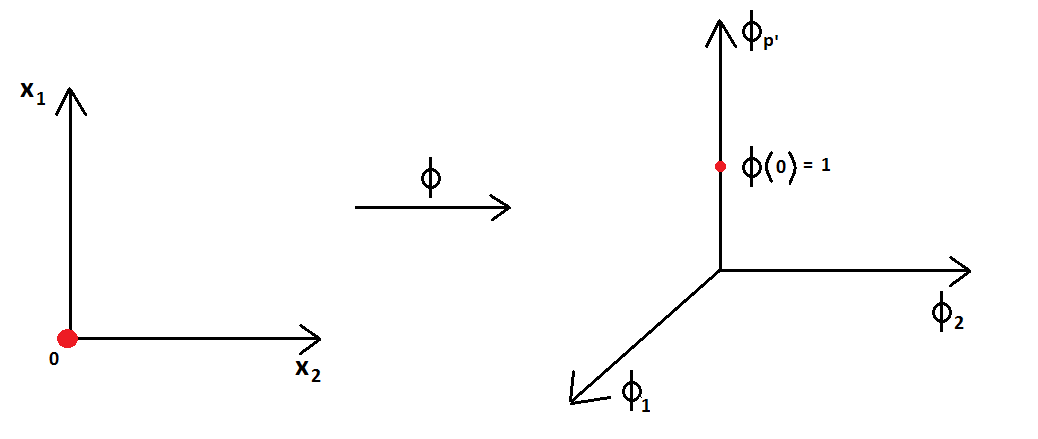
\includegraphics[width=0.9\linewidth]{images/Kernel_nonHomogene}
%%	\caption{Illustration of samples in $\mathbb{R}^2$. The transformation $\phi$ for a polynomial kernel $K(\textbf{x}_i,\textbf{x}_j)=(\textbf{x}_i^T \textbf{x}_j + c)^d$ with $c=1$ and $d=2$ can be written explicitly: $\phi(\textbf{x}_i)= [x_{i1}^2, x_{i2}^2, \sqrt{2} x_{i1} x_{i2}, 1]^T$. The origin point $\textbf{x}_i=[0,0]^T$ is projected in the Hilbert space as $\phi(\textbf{x}_i=\textbf{0}) = [0, 0, 0, 1]^T$.}
%%	\label{fig:Kernel_nonHomogene}
%%\end{figure}
%%
%%However, to define proper metrics that respects the properties of metrics (Section \ref{sec:property_metric}), specific kernels must be used. Our work don't propose any solutions to this problem but open the field for new research on this topic. 

\subsection{Link between SVM and the quadratic formalization}
%\subsubsection{Motivations}
%\begin{itemize}
%	\item Faire remarquer que le problème LP ressemble à un problème SVM
%	\item Faire la démonstration de l'équivalence (ou mettre la démonstration en annexe).
%	\item Expliquer les différences entre la résolution LP/QP et la résolution SVM. (ajout de sur-contraintes dans le problème SVM)
%	\item Expliquer pourquoi on va préférer le cadre SVM. Expliquer mathématiquement et avec des interprétations géométriques. 
%	\item Cadre connu
%	\item Utilisation de librairie standard de Machine Learning
%	\item Extension directe à l'apprentissage de métrique non linéaire grâce au kernel trick
%\end{itemize}

Many parallels have been studied between Large Margin Nearest Neighbors ({\sc lmnn}) and \textsc{svm} (Section \ref{sec:LMNN_SVM}). \textsc{svm} is a well known framework: its has been well implemented in many libraries (\textit{e.g.}, {\sc liblinear} \cite{Fan2008} and {\sc libsvm} \cite{Hsu2008}), well studied for its generalization properties and extension to non-linear solutions. Similarly, we can make a link between the quadratic formalization and a \textsc{svm} problem where the form of the metric $D$ is defined \textit{a priori}.

We show in Appendix \ref{chap:app:svm_link} that solving the \textsc{svm} problem in Eq.~\ref{eq:SVMSofMarginProblem0} for $\textbf{w}$ and $b$ solves a similar problem with a quadratic regularization in Eq.~\ref{eq:quadratic} for $D(\textbf{x}_{ij})=-\frac{1}{2}(\textbf{w}^T\textbf{x}_{ij}+b)$. 
\begin{equation}
\begin{aligned}
&\displaystyle \argmin_{\textbf{w},b,\xi} 
\left\lbrace \frac{1}{2}||\textbf{w}||_2^2
+ C \sum\limits_{\substack{i \\j \in Pull_i \text{  or  } \\ j \in Push_i}}p_i\xi_{ij} \right\rbrace \\
& \text{s.t.  }  \forall i,j \in Pull_i \text{  or  } j \in Push_i: \\
& y_{ij}(\textbf{w}^T\textbf{x}_{ij}+b) \geq 1-\xi_{ij}
\end{aligned}
\label{eq:SVMSofMarginProblem0}
\end{equation}
\noindent where $p_i$ is a weight factor for each slack variable $\xi_{ij}$ (in classical \textsc{svm}, $p_i=1$). The loss part in the \textsc{svm} formulation can be split into 2 terms involving the sets $Pull_i$ and $Push_i$:

\begin{equation}
\begin{aligned}
&\displaystyle \argmin_{\textbf{w},b,\xi} 
\left\lbrace \frac{1}{2}||\textbf{w}||_2^2
+ C \sum\limits_{\substack{i \\j \in Pull_i}}p_i^+\xi_{ij}
+ C \sum\limits_{\substack{i \\l \in Push_i}}p_i^-\xi_{il} \right\rbrace \\
& \text{s.t.  }: \\
& \forall i,j \in Pull_i: y_{ij}(\textbf{w}^T\textbf{x}_{ij}+b) \geq 1-\xi_{ij}\\
& \forall i,l \in Push_i: y_{il}(\textbf{w}^T\textbf{x}_{il}+b) \geq 1-\xi_{il}\\
\end{aligned}
\label{eq:SVMSofMarginProblem1}
\end{equation}
\noindent where $p_i^+$ and $p_i^-$ are the weight factors for pull pairs $Pull_i$ and push pairs $Push_i$. To obtain an equivalence, we set $p_i^-$ as the half of the number pairs in $Pull_i$ and $p_i^+$ as the half of the number of time series $L$ in $Push_i$:
\begin{align}
	p_i^- &= \frac{k}{2} = \sum_{j \in Pull_i} \frac{1}{2} \label{eq:pi_plus}\\
	p_i^+ &= \frac{L}{2} = \frac{1}{2}\sum_l \frac{1-y_{il}}{2} \label{eq:pi_moins}
\end{align}

\noindent In particular, let's underline the main similarities and differences:
\begin{itemize}
	\item[-] Both problems share a same set of constraints between triplets:
		\begin{equation*}
			\forall i,j \in Pull_i,l \in Push_i:
			D(\textbf{x}_{il})-D(\textbf{x}_{ij}) \geq 1-\xi_{ijl}
		\end{equation*}
	\item[-] The \textsc{svm} problem includes an additional set of constraints that is not present in the quadratic formalization. \textsc{svm} takes into account pull pairs $\textbf{x}_{ij}$ and push pairs $\textbf{x}_{kl}$ that doesn't belong to the same neighborhood:
		\begin{align*}
			\forall i,j \in Pull_i,k,l \in Push_k, i \neq k: 
			D(\textbf{x}_{kl})-D(\textbf{x}_{ij}) \geq 1-\frac{\xi_{kl}+\xi_{ij}}{2}	
		\end{align*}
	\item[-] The \textsc{svm} problem includes in the loss term additional slack variables $\xi_{ijl}$ that are not present in the quadratic formalization because of the additional set of constraints. It is not only a push term.
	% \item Both problems share the same loss/push term: $\sum\limits_{\substack{i \\ j \in Pull_i \\ l \in Push_i}} \frac{1+y_{il}}{2} \xi_{ijl} $
	\item[-] The two problems involves different regularized term: in the quadratic formalization, the regularizer involves a pull action (Eqs. \ref{eq:regularizer1} \& \ref{eq:regularizer2}), not present in \textsc{svm}.
	% in \textsc{svm}, the regularizer $\frac{1}{2} ||\textbf{w}||_2^2$ only involves the weight vector $\textbf{w}$, whereas in the quadratic formalization, the regularizer involves also the pull pairs (Eqs. \ref{eq:regularizer1} \& \ref{eq:regularizer2})
	\item[-] Both problems suppose at first a linear combination for $D$.
\end{itemize}

Concerning the properties of the metric $D$, positivity is not ensured in the primal and dual formulation.
% as \textsc{svm} tries to find an hyperplane, the constraint $w_h \geq 0$ does not hold. 
Symmetry and reflexivity is ensured.

%--------------------------------------------------------------------------------
\section{SVM-based formalization for M$^2$TML}
In this section, we present a solution based on \textsc{svm} where the form of the metric $D$ is not known \textit{a priori}. We formulate the problem as a \textsc{svm} problem to solve a large margin problem between $Pull_i$ and $Push_i$ sets, and then, induce a combined metric $D$ for the obtained \textsc{svm} solution. 
% First, we learn an hyperplane that separates the sets $Pull_i$ and $Push_i$. Secondly, we propose a solution to build a metric $D$ from the obtained hyperplane so that the metric $D$ satisfy the required properties of a metric. 
Thanks to the \textsc{svm} framework, the proposition can be naturally extended to learn both, linear or non-linear function for the metric $D$.

\subsection{Support Vector Machine (\textsc{svm}) resolution}
Let $\{\textbf{x}_{ij}; y_{ij} = \pm 1\}$, $\textbf{x}_{ij} \in Pull_i \cup Push_i$ be the training set, with $y_{ij} = -1$ for $\textbf{x}_{ij} \in$ $Push_i$ and $+1$ for $\textbf{x}_{ij} \in$ $Pull_i$. For a maximum margin between the sets $Pull_i$ and $Push_i$, the problem is formalized in the dissimilarity space $\mathcal{E}$:
\begin{equation}
	\begin{aligned}
	& \argmin_{\textbf{w},b,\boldsymbol{\xi}} \frac{1}{2}||\textbf{w}||_2^2 + C \sum\limits_{i,j} \xi_{ij} \label{eq:svm_pairwise}\\
	&\textbf{s.t. } y_{ij}(\textbf{w}^T \textbf{x}_{ij} + b) \geq 1-\xi_{ij} \\
	&\xi_{ij} \geq 0
	\end{aligned}
\end{equation}

\noindent In the linear case, a $L_1$ regularization in Eq. \ref{eq:svm_pairwise} leads to a sparse and interpretable \textbf{w} that uncovers the modalities, periods and scales that differentiate best pull from push pairs for a robust nearest neighbors classification.
%\begin{equation}
%\begin{aligned}
%	& \argmin_{\textbf{w},b,\boldsymbol{\xi}} ||\textbf{w}||_1 + C \sum\limits_{i,j} \xi_{ij} \label{eq:svm_pairwiseL1} \\
%	&\textbf{s.t. } y_{ij}(\textbf{w}^T \textbf{x}_{ij} + b) \geq 1-\xi_{ij} \\
%	&\xi_{ij} \geq 0
%	\end{aligned}
%\end{equation}
Note that in practice, the local neighborhoods for each sample $\textbf{x}_i$ can have very different scales. Thanks to the unit radii normalization $\textbf{x}_{ij}/r_i$, where $r_i$ denotes the norm of the $m$-th neighbors in $Pull_i$, the \textsc{svm} ensures a global large margin solution involving equally local neighborhood constraints (\textit{i.e.} local margins).

\noindent Note that any multi-class problem is transformed in the dissimilarity space as a binary classification problem.

\subsection{Linearly separable Pull and Push sets}
Let $\textbf{x}_{test}$ be a new sample, $\textbf{x}_{i,test} \in \mathcal{E}$ gives the proximity between $\textbf{x}_{i}$ and $\textbf{x}_{test}$ based on the $p$ multi-modal and multi-scale metrics $d_h$. We denote $\textbf{P}_\textbf{w}(\textbf{x}_{i,test})$ the orthogonal projection of $\textbf{x}_{i,test}$ on the axis of direction \textbf{w} and $||\textbf{P}_\textbf{w}(\textbf{x}_{i,test})||$ its norm. We review in this section different interpretations in the dissimilarity space. \\

\noindent \textbf{M$^2$TML metric definition} \\
Given a test pair $\textbf{x}_{i,test}$, the norm of the pair allows to estimate the proximity between $\textbf{x}_{i}$ and $\textbf{x}_{test}$. In particular, for \textsc{m$^2$tml}, two quantities are used to define the dissimilarity measure: the projected norm and the distance to the margin.

%\noindent \textbf{Projected norm.} 
\noindent The projected norm $||\textbf{P}_\textbf{w}(\textbf{x}_{i,test})||$ of $\textbf{x}_{i,test}$ on the direction $\textbf{w}$ limits the comparison of $\textbf{x}_{i}$ and $\textbf{x}_{test}$ to the features separating pull and push sets (Fig. \ref{fig:projected_norm}), it is defined as:
\begin{align}
	||\textbf{P}_\textbf{w}(\textbf{x}_{i,test})|| 
	&= 
	\frac{||\textbf{w}^T\textbf{x}_{i,test}||}{||\textbf{w}||}
	\label{eq:projected_norm}
\end{align}
\noindent with:
\begin{align}
	\textbf{P}_\textbf{w}(\textbf{x}_{i,test}) 
	&= 
	\frac{<\textbf{w},\textbf{x}_{i,test}>}{||\textbf{w}||^2} \textbf{w} = \frac{\textbf{w}^T\textbf{x}_{i,test}}{||\textbf{w}||^2} \textbf{w}
	\label{eq:projected}
\end{align}	
\begin{figure}[h!]
	\centering
	\includegraphics[width=0.6\linewidth]{projected_norm}
	\caption{The projected vector $\textbf{P}_\textbf{w}(\textbf{x}_{ij})$ and $\textbf{P}_\textbf{w}(\textbf{x}_{ij'})$}
	\label{fig:projected_norm}
\end{figure}

\noindent Although the norm $||\textbf{P}_\textbf{w}(\textbf{x}_{i,test})||$ satisfies positivity, it doesn’t guarantee lower distances for pull pairs than for push pairs as illustrated in Fig \ref{fig:Dissimilarity_def_norm_scalar_product}. 

\begin{figure}[h!]
	\centering
	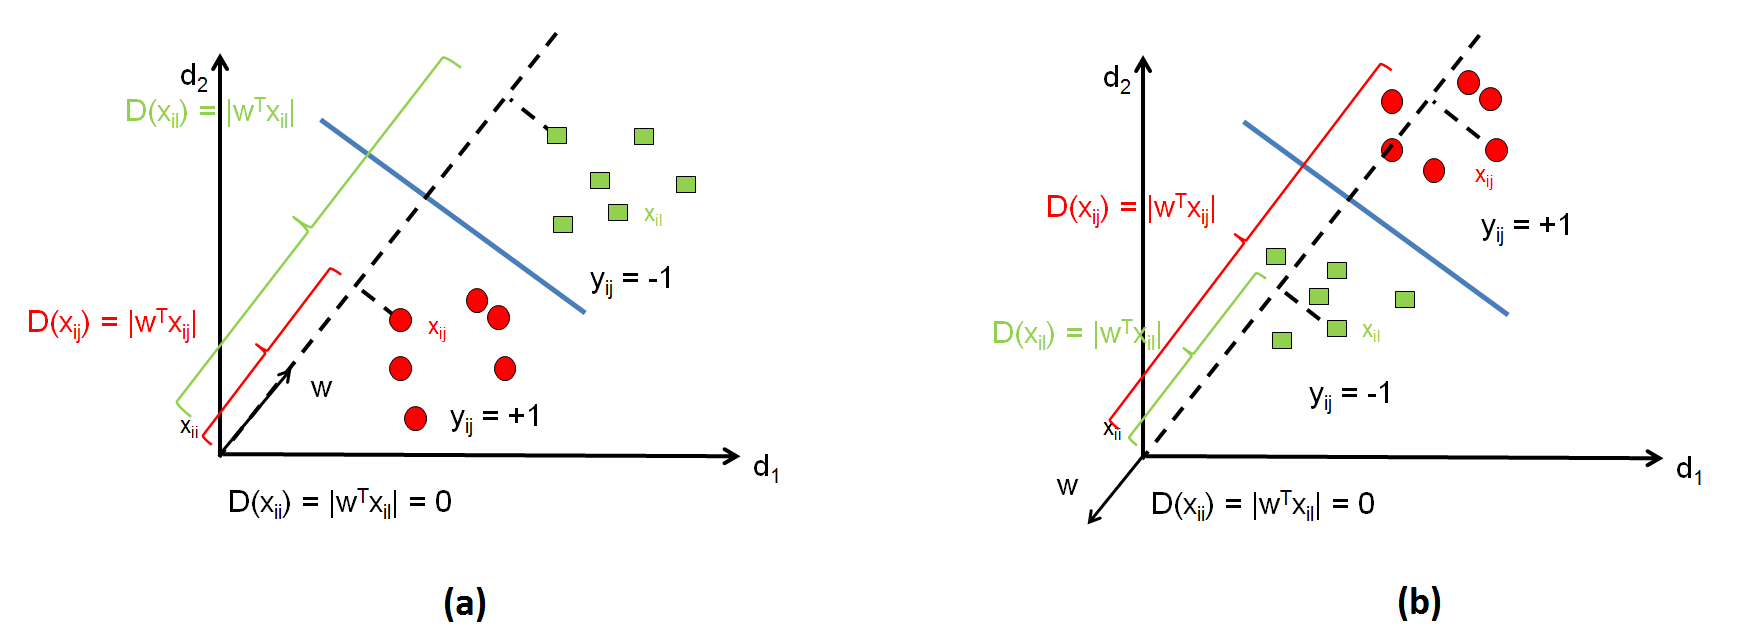
\includegraphics[width=1\linewidth]{images/Dissimilarity_def_norm_scalar_product}
	\caption{Example of \textsc{svm} solutions and of the resulting metric $D$ defined by the norm of the projection on $\textbf{w}$. Fig. (a) represents common expected configuration where pull pairs $Pull_i$ are situated in the same side as the origin $\textbf{x}_{ii}=0$. In Fig. (b), the vector $\textbf{w}=[-1 -1]^T$ indicates that push pairs $Push_i$ are on the side of the origin point. One problem arises in Fig. (b): distance of push pairs $D(\textbf{x}_{il})$ is lower than the distance of pull pairs $D(\textbf{x}_{ij})$.}
	\label{fig:Dissimilarity_def_norm_scalar_product}
\end{figure}

%\noindent \textbf{Distance to the margin.} 
Note that the distance of the projection to the margin $\textbf{w}^T \textbf{P}_\textbf{w}(\textbf{x}_{i,test}) + b$ gives the membership of the projected vector $\textbf{P}_\textbf{w}(\textbf{x}_{i,test})$ in the pull or push side. However, it can't used as a dissimilarity (non-positivity). 
% To take into account of the localization of the pair $\textbf{x}_{i,test}$ on the pull or push side, the distance of the projection to the margin is considered: $\textbf{w}^T P_w(\textbf{x}_{i,test}) + b$. Even if the distance to the margin gives the membership of $P_w(\textbf{x}_{i,test})$ to the pull or push side, it can't used as a dissimilarity (non-positivity). \\

%Given a test pair $\textbf{x}_{i,test}$, the distance to the margin $\textbf{w}^T\textbf{x}_{i,test} + b$ is a signed quantity. It doesn't verify the positivity property and can't thus be used to define the metric $D$.
%%First, the learned metric $D$ can be defined as the distance to the hyperplane:
%%\begin{equation}
%%D(\textbf{x}_{i,test}) = \textbf{w}^T\textbf{x}_{i,test} + b
%%\end{equation}
%%The obtained metric $D$ doesn't necessarily satisfy the distinguishability ($D(\textbf{x}_{ii}=0)$) and positivity ($D(\textbf{x}_{ij} \geq 0)$) property, especially when push pairs $Push_i$ are situated nearer to the origin point than pull pairs $Pull_i$ (Fig. \ref{fig:Dissimilarity_def_scalar_product}).
%%\begin{figure}[h!]
%%	\centering
%%	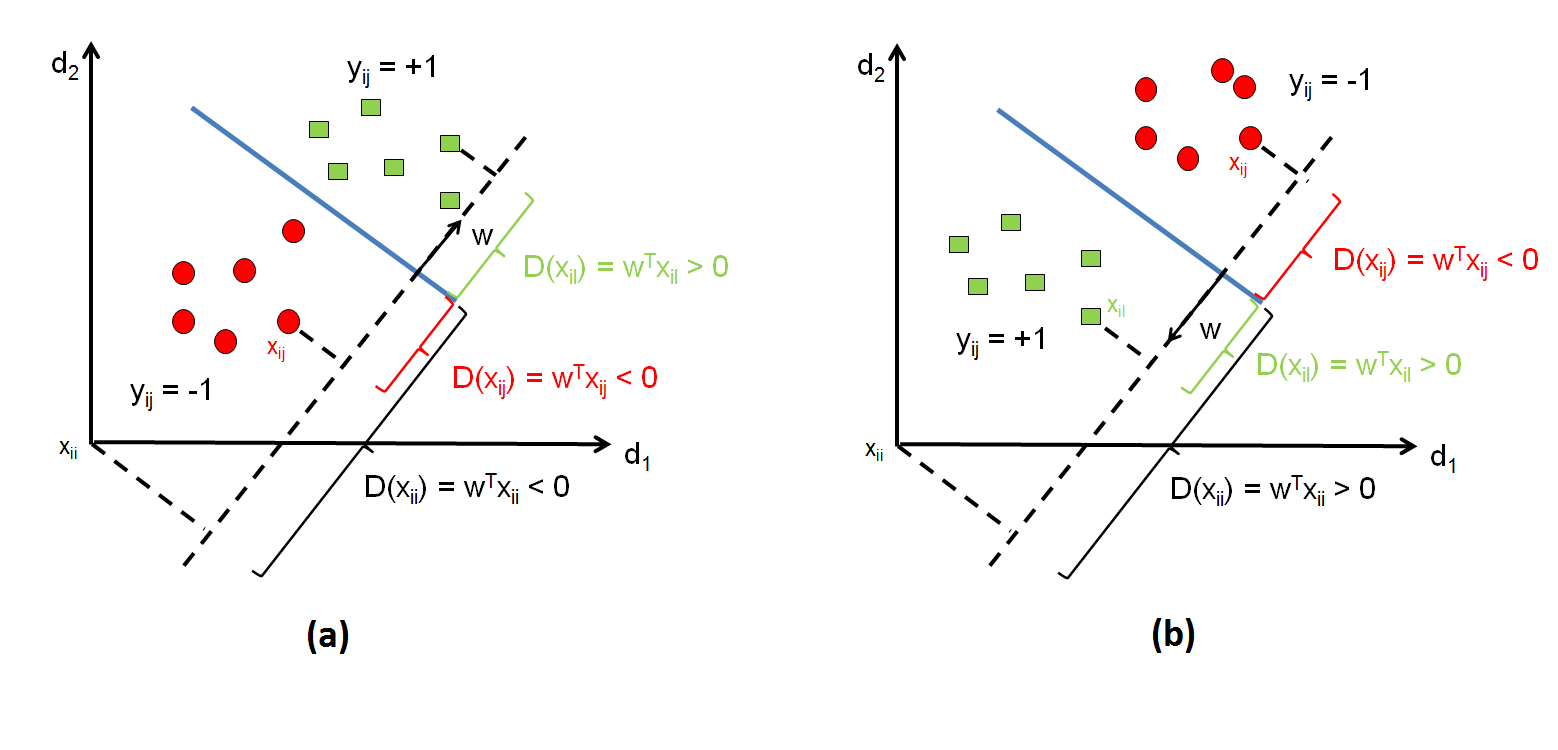
\includegraphics[width=1\linewidth]{images/Dissimilarity_def_scalar_product}
%%	\caption{Example of \textsc{svm} solutions and of the resulting metric $D$ defined by a scalar product. Fig. (a) represents common expected configuration where pull pairs $Pull_i$ are situated in the same side as the origin $\textbf{x}_{ii}=0$. In Fig. (b), the vector $\textbf{w}=[-1 -1]^T$ indicates that $Push_i$ pairs are on the side of the origin point. For the two configurations, two problems arises: First, for pull pairs $Pull_i$, $D(\textbf{x}_{ij}) \leq 0$. Secondly, for the origin point $\textbf{x}_{ii}$, we obtain $D(\textbf{x}_{ii}) \neq 0$.}
%%	\label{fig:Dissimilarity_def_scalar_product}
%%\end{figure}
%Secondly, we recall the formula of the projection of a pair $\textbf{x}_{i,test}$ on the vector $\textbf{w}$:
%\begin{align}
%	\textbf{P}_\textbf{w}(\textbf{x}_{i,test}) = \frac{<\textbf{w},\textbf{x}_{i,test}>}{||\textbf{w}||^2} \textbf{w} = \frac{\textbf{w}^T\textbf{x}_{i,test}}{||\textbf{w}||^2} \textbf{w}
%	\label{eq:projected}
%\end{align}
%The norm of the projection, measures the distance of the pair $\textbf{x}_{i,test}$ from the origin point $\textbf{x}_{ii}$ and takes into account the discriminative features:
%\begin{equation}
%	||\textbf{P}_\textbf{w}(\textbf{x}_{i,test})|| = \frac{||\textbf{w}^T\textbf{x}_{i,test}||}{||\textbf{w}||}
%	\label{eq:projected_norm}
%\end{equation}
%\noindent As illustrated in Fig. \ref{fig:projected_norm}, by considering the norm of the projection, a pair $\textbf{x}_{ij}$ becomes as similar as a pair $\textbf{x}_{ij'}$ whereas their norm $||\textbf{x}_{ij}||$ and $||\textbf{x}_{ij'}||$ shows their are not similar.


%\noindent \textbf{Exponential transformation.} 
We propose to add an exponential term to operate a "push" on push pairs based on their distances to the separator hyperplan, that leads to the dissimilarity measure $D$ of required properties:
\begin{equation}
D(\textbf{x}_{i,test}) = 
||\textbf{P}_\textbf{w}(\textbf{x}_{i,test})||.
\exp(\lambda[-(\textbf{w}^T\textbf{P}_\textbf{w}(\textbf{x}_{i,test}) + b)]_+)
\text{ \quad  } \lambda > 0
\label{eq:dissimilarity_learn}
\end{equation}
where $\lambda$ controls the "push" term and $\textbf{w}^T\textbf{P}_\textbf{w}(\textbf{x}_{i,test}) + b$ defines the distance between the orthogonal projected vector and the separator hyperplane; $[t]_+ = \max(0; t)$ being the positive operator. Note that, for a pair lying into the pull side ($y_{ij} = +1$), $[-(\textbf{w}^T\textbf{P}_\textbf{w}(\textbf{x}_{i,test}) + b)]_+ = 0$, the exponential term is vanished (i.e. no "pull" action) and the dissimilarity leads to the norm term. For a pair situated in the push side ($y_{ij} = -1$), the norm is expanded by the push term, all the more the distance to the hyperplane is high.

\begin{figure}[h!]
	\centering
	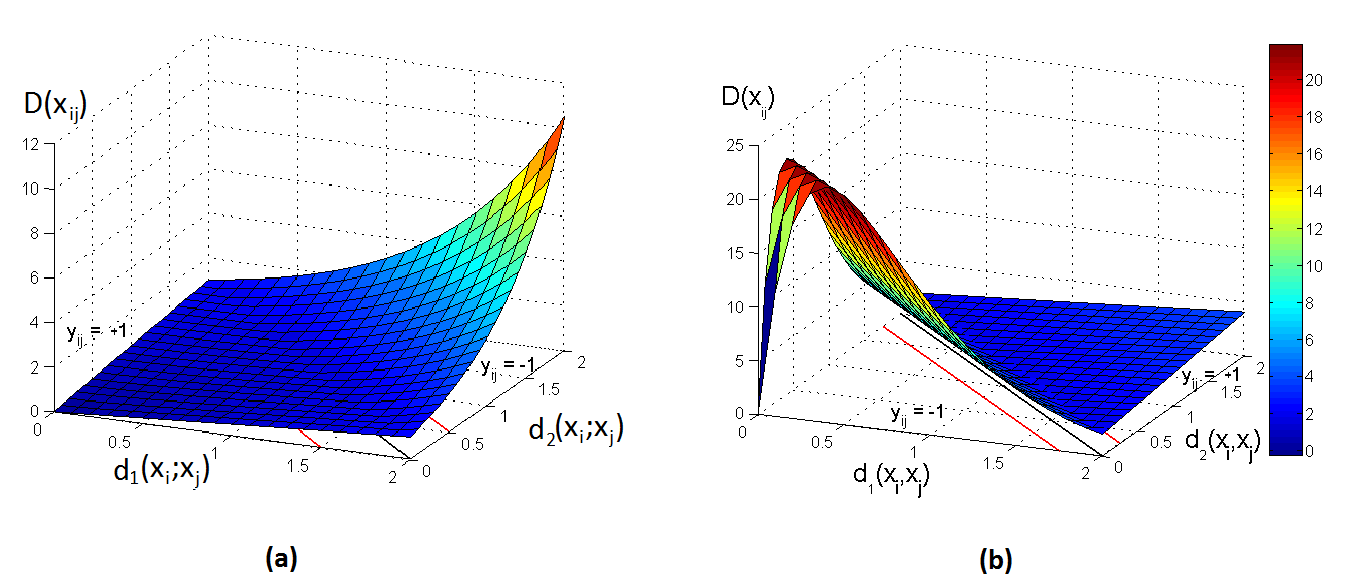
\includegraphics[width=0.95\linewidth]{images/3D_diss}
	\caption{The behavior of the learned metric $D$ ($p = 2$; $\lambda = 2.5$) with respect to common (a) and challenging (b) configurations of pull and push pairs.}
	\label{fig:3D_diss}
\end{figure}

%\begin{figure}[h!]
%	\centering
%	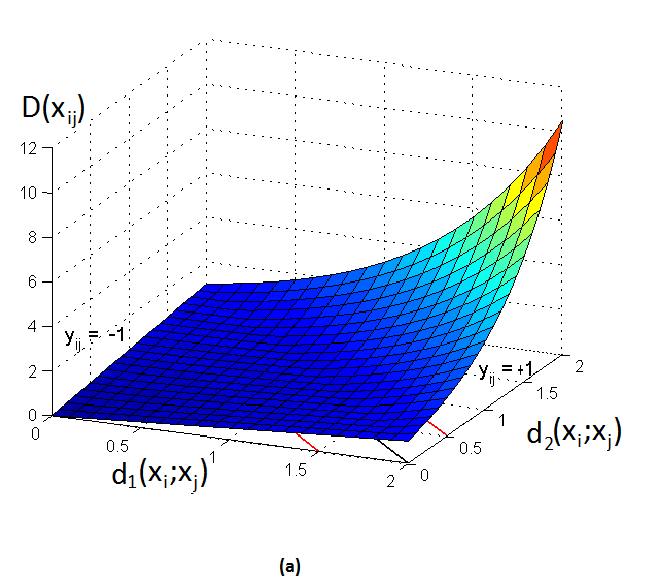
\includegraphics[width=0.6\linewidth]{images/3D_positive1}
%	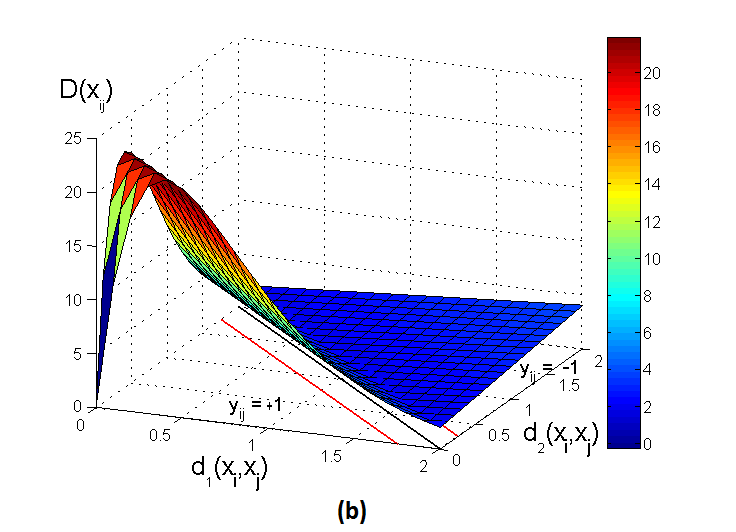
\includegraphics[width=0.6\linewidth]{images/3D_negative}
%	\caption{The behavior of the learned metric $D$ ($p = 2$; $\lambda = 2.5$) with respect to common (a) and challenging (b) configurations of positive and negatives pairs.}
%	\label{fig:3D_diss}
%\end{figure}

Fig. \ref{fig:3D_diss}, illustrates for $p = 2$ the behavior of the learned dissimilarity according to two extreme cases. The first one (Fig. \ref{fig:3D_diss}-a), represents common expected configuration where pairs $Pull_i$ are situated in the same side as the origin. The dissimilarity increases proportionally to the norm in the pull side, then exponentially on the push side. Although the expansion operated in the push side is dispensable in that case, it doesn’t affect nearest neighbors classification. Fig. \ref{fig:3D_diss}-b, shows a challenging configuration where pairs $Push_i$ are situated in the same side as the origin. The dissimilarity behaves proportionally to the norm on the pull side, and increases exponentially from the hyperplane until an abrupt decrease induced by a norm near 0. Note that the region under the abrupt decrease mainly uncovers false pairs $Push_i$, \textit{i.e.}, pairs of norm zero labeled differently.

\subsection{Non-linearly separable Pull and Push sets}
The above solution holds true for any kernel $\kappa$ and allows to extend the dissimilarity $D$ given in Eq. \ref{eq:dissimilarity_learn} to non linearly separable pull and push pairs. Let $\kappa$ be a kernel defined in the dissimilarity space $\mathcal{E}$ and the related Hilbert space (feature space) $\mathcal{H}$. For a non linear combination function of the metrics $d_h, h = 1,\ldots,p$ in $\mathcal{E}$, we define the dissimilarity measure $D_\mathcal{H}$ in the feature space $\mathcal{H}$ as:

\begin{equation}
\begin{aligned}
D_\mathcal{H}(\textbf{x}_{i,test}) = 
& \left| (||\textbf{P}_\textbf{w}(\Phi(\textbf{x}_{i,test}))||-||\textbf{P}_\textbf{w}(\Phi(\textbf{0}))||) \right|   . \\
& \exp\left( \lambda \left[  -\left( \sum_{ij}y_{ij} \alpha_{ij} \kappa(\textbf{x}_{ij},\textbf{x}_{i,test}) + b \right)  \right] _+\right) 
\text{ \quad  } \lambda > 0
\label{eq:dissimilarity_learn_NonLinear}
\end{aligned}
\end{equation}

\noindent with $\Phi(\textbf{w})$ the image of \textbf{w} into the feature space $\mathcal{H}$. Based on Eq. \ref{eq:projected}, substituing Eq. \ref{Eq:eqn_w} back into $\textbf{w}$, the inner product gives $<\textbf{w};\Phi(\textbf{x}_{i,test})> = \sum_{ij} y_{ij} \alpha_{ij} \kappa(\textbf{x}_{ij},\textbf{x}_{i,test})$ and the norm of $\textbf{w}$ gives $||\textbf{w}||= \sqrt{\sum_{ijkl} \alpha_{ij} \alpha_{kl} y_{ij} y_{kl} \kappa(\textbf{x}_{ij},\textbf{x}_{kl})}$. Replacing back into Eq. \ref{eq:projected_norm}, the norm of the orthogonal projection of $\Phi(\textbf{x}_{i,test})$ on $\Phi(\textbf{w})$ gives:
\begin{align}
||\textbf{P}_\textbf{w}(\Phi(\textbf{x}_{i,test}))|| & = \frac
{\sum_{ij} y_{ij} \alpha_{ij} \kappa(\textbf{x}_{ij},\textbf{x}_{i,test})}
{\sqrt{\sum_{ijkl} \alpha_{ij} \alpha_{kl} y_{ij} y_{kl}
		\kappa(\textbf{x}_{ij},\textbf{x}_{kl})
	}}
\end{align}
Note that as $\Phi(\textbf{0})$ doesn’t meet the origin in the feature space $\mathcal{H}$, the norms in Eq. \ref{eq:dissimilarity_learn_NonLinear} are centered with respect to $\Phi(\textbf{0})$ to ensure the reflexivity property. 
% Note also that the denominator is positive since it is equal to $||\textbf{w}||$.
It is easy to show that both $D$ and $D_\mathcal{H}$ ensure the properties of a dissimilarity (positivity, reflexivity, symmetry).
% Concerning the properties of $D$ and $D_\mathcal{H}$, it can be shown that reflexivity and symmetry is ensured. Positivity is ensured as $D$ is a product of two positive terms.

Note that the framework to define the metric $D$ and $D_\mathcal{H}$ can also be used in the linear and quadratic formalization. However, the obtained solution for $D$ and $D_\mathcal{H}$ can be far away from the original form of $D$ that was optimized in the optimization problem.

% Note that other propositions for $D$ and $D_\mathcal{H}$ are possible. For example, we could not consider the max operator and allow $\lambda \in \mathbb{R}$. Thus, for negative values of $\lambda$, the exponential term will have a pull action. Note that in both case, the dissimilarity measure can lead to extreme values, making a risk to polarize the dissimilarity. In practice, our proposed $D$ and $D_\mathcal{H}$ provides suitable solutions for the considered datasets. Moreover, note that the framework to define the metric $D$ and $D_\mathcal{H}$ can also be used in the linear and quadratic formalization. However, the obtained solution for $D$ and $D_\mathcal{H}$ can be far away from the original form of $D$ that was optimized in the optimization problem.


%---------------------------------------------------------------------------
\section{SVM-based solution and algorithm for M$^2$TML}
% \subsection{Algorithm}
\noindent In this section, we review the main steps of this latter retained \textsc{svm} solution. In particular, we detail two pre-processing steps needed to adapt the \textsc{svm} framework to our metric learning problem that are the pairwise space normalization and the neighborhood scaling.

\noindent \textbf{Pairwise space normalization.} 
The scale between the $p$ basic metrics $d_h$ can be different. Thus, there is a need to scale the data within the pairwise space and ensure comparable ranges for the $p$ basic metrics $d_h$. In our experiment, we use dissimilarity measures with values in $[0;+\infty[$. Therefore, we propose to Z-normalize their log distributions as explained in Section \ref{sec:data_normalization}. \\

\noindent \textbf{Neighborhood scaling.} 
In real datasets, local neighborhoods can have very different scales as illustrated in Fig. \ref{fig:Neighborhood_scaling_problem}. To make the pull neighborhood spreads comparable, we propose for each $\textbf{x}_i$ to scale each pairs $\textbf{x}_{ij}$ such that the $L_2$ norm (radius) of the farthest $m$-th nearest neighbor is 1:
\begin{equation}
\textbf{x}_{ij}^{norm} = \left[ \frac{d_1(\textbf{x}_{i},\textbf{x}_{j})}{r_i}, \ldots, \frac{d_p(\textbf{x}_{i},\textbf{x}_{j})}{r_i}\right] ^T \label{eq:normalization_radius}
\end{equation}
where $r_i$ is the radius associated to $\textbf{x}_i$ corresponding to the maximum norm of its $m$-th nearest neighbor of same class in $Pull_i$:
\begin{equation}
r_i = \max_{\textbf{x}_{ij} \in Pull_i} ||\textbf{x}_{ij}||_2
\end{equation}
For simplification purpose, we denote $\textbf{x}_{ij}$ as $\textbf{x}_{ij}^{norm}$. Fig. \ref{fig:Neighborhood_scaling} illustrates the effect of neighborhood scaling in the dissimilarity space.
\begin{figure}[h!]
	\centering
	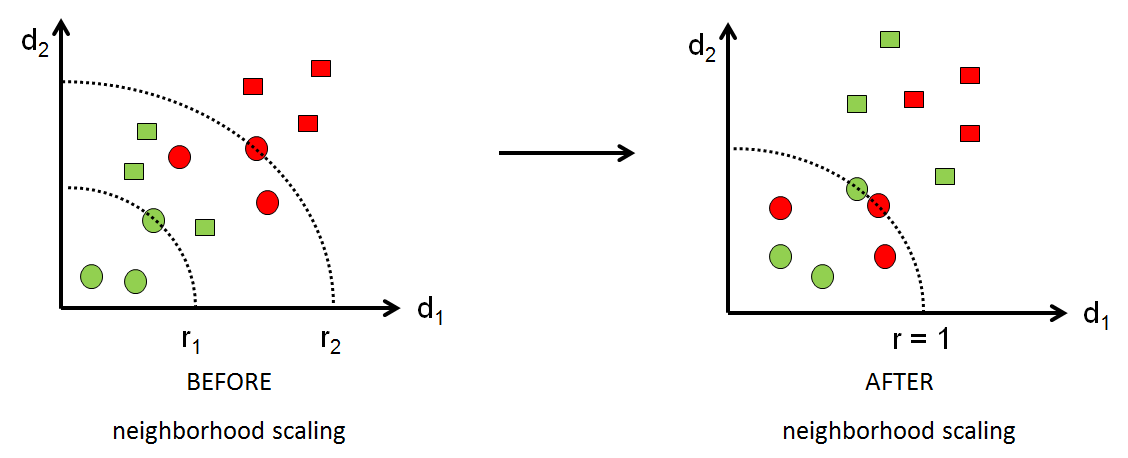
\includegraphics[width=1\linewidth]{images/Neighborhood_scaling}
	\caption{Effect of neighborhood scaling before (left) and after (right) on the neighborhood of two time series $\textbf{x}_1$ (green) and $\textbf{x}_2$ (red). Circle represent pull pairs $Pull_i$ and square represents push pairs $Push_i$ for $m=3$ neighbors. Before scaling, the problem is not linearly separable. The spread of each neighborhood are not comparable. After scaling, the target neighborhood becomes comparable and in this example, the problem becomes linearly separable between the circles and the squares.}
	\label{fig:Neighborhood_scaling}
\end{figure}



\noindent Finally, Algorithm 1 summarizes the main steps to learn a multi-modal and multi-scale metric $D$ for a robust nearest neighbors classification. Algorithm 2 details the steps to classify a new sample $\textbf{x}_{test}$ using the learned metric $D$.
\begin{algorithm}[h!]
	\begin{algorithmic}[1]
		\caption{Multi-modal and Multi-scale Temporal Metric Learning ({\sc m}$^2${\sc tml}) for $k$-NN classification}
		\label{algo:MMTML}
		\STATE Input:  
		$\{\textbf{x}_i, y_i\}_{i=1}^n$ $n$ labeled time series \\ \hspace{1.1cm} $d_1, ...,d_p$  metrics as described in Eqs. \ref{eq:A}, \ref{eq:F}, \ref{eq:B}, \ref{eq:A2} \\
		\hspace{1.1cm} a kernel $\kappa$
		\STATE Output:  the learned dissimilarity $D$ or $D_{\mathcal{H}}$ depending of $\kappa$ \\
		\STATE  {\it Dissimilarity embedding} \\   
		Embed pairs $(\textbf{x}_i,\textbf{x}_j)$ $i,j \in {1,...,n}$ into $\mathcal{E}$ as described in Eq. \ref{eq:projection} and normalize $d_h$s
		\STATE  {\it Build $Pull_i$ and $Push_i$ sets} \\   
		Build the sets of pairs $Pull_i$ and $Push_i$ as described in Eq. \ref{eq:pull1} \& \ref{eq:push1} and scale the radii to 1 (Eq. \ref{eq:normalization_radius}).
		% \STATE Define the training set $\{\textbf{x}_{ij}, y_{ij}= \pm 1\}$ with  $\textbf{x}_{ij} \in m$NN+ $\cup$ $m$NN- 
		\STATE {\it \textsc{svm} learning} \\   
		Train a \textsc{svm} for a large margin classifier between  $Pull_i$ and $Push_i$ sets (Eq. \ref{eq:svm_pairwise})
		\STATE {\it Dissimilarity definition} \\ 
		Consider Eq. \ref{eq:dissimilarity_learn} (resp. Eq. \ref{eq:dissimilarity_learn_NonLinear}) to define $D$ (resp. $D_{\mathcal{H}}$) a linear (resp. non linear) combination function of the metrics $d_h$s.
	\end{algorithmic}
\end{algorithm}


\begin{algorithm}[h!]
	\begin{algorithmic}[1]
		\caption{$k$-NN classification using the learned metric $D$ or $D_{\mathcal{H}}$}
		\STATE Input:  
		$\{\textbf{x}_i, y_i\}_{i=1}^n$ $n$ labeled time series \\
		\hspace{1.1cm} $\{\textbf{x}_{test}, y_{test}\}$ a labeled time series to test \\
		\hspace{1.1cm} $d_1, ...,d_p$  metrics as described in Eqs. \ref{eq:A}, \ref{eq:F}, \ref{eq:B}, \ref{eq:A2} \\
		\hspace{1.1cm} the learned dissimilarity $D$ or $D_{\mathcal{H}}$ depending of the kernel $\kappa$
		\STATE Output: Predicted label $\hat{y}_{test}$
		\STATE  {\it Dissimilarity embedding} \\   
		Embed pairs $(\textbf{x}_i,\textbf{x}_{test})$ $i\in {1,...,n}$ into $\mathcal{E}$ as described in Eq. \ref{eq:projection} and normalize $d_h$s using the same normalization parameters in Algorithm 1
		\STATE {\it Combined metric computation} \\ 
		Consider Eq. \ref{eq:dissimilarity_learn} (resp. Eq. \ref{eq:dissimilarity_learn_NonLinear}) to compute $D(\textbf{x}_i,\textbf{x}_{test})$ (resp. $D_{\mathcal{H}}(\textbf{x}_i,\textbf{x}_{test})$) a linear (resp. non linear) combination function of the metrics $d_h(\textbf{x}_i,\textbf{x}_{test})$.
		\STATE {\it Classification} \\
		Consider the $k$ lowest dissimilarities $D(\textbf{x}_i,\textbf{x}_{test})$ (resp. $D_{\mathcal{H}}(\textbf{x}_i,\textbf{x}_{test})$). Extract the labels $y_i$ of the considered $\textbf{x}_i$ and make a vote scheme to predict the label $\hat{y}_{test}$ of $\textbf{x}_{test}$
	\end{algorithmic}
\end{algorithm}

% Algorithm 1 can be extended for multivariate and regression problem. First, for multivariate problem, each unimodal metric $d_h$ can be computed for each variable. Then, the above framework can be applied. For regression problem, the label $y_i$ for each time series $\textbf{x}_i$ is a continuous value. The only modification is at the neighborhood steps, when defining the sets $Pull_i$ and $Push_i$. For that, we propose in the following two different strategies to define the pairwise labels $y_{ij}$.

%\subsection{Extension to regression problems}
%In the dissimilarity space, each vector $\textbf{x}_{ij}$ can be labeled $y_{ij}$ by following the rule: "if $\textbf{x}_i$ and $\textbf{x}_j$ are similar ($Pull_i$), the vector $\textbf{x}_{ij}$ is labeled -1; and +1 otherwise ($Push_i$)." \\
%Until here, we solve the metric learning for classification problems. The concept of similarity between samples $\textbf{x}_i$ and $\textbf{x}_j$ is driven by the class label $y_i$ and $y_j$ in the original space:
%\begin{equation}
%y_{ij} = 
%\left\{
%\begin{split}
%-1 \text{\quad if } y_i = y_j\\ 
%+1 \text{\quad if } y_i \neq y_j
%\end{split}
%\right.
%\end{equation}
%For regression problems, each sample $\textbf{x}_i$ is assigned to a continuous value $y_i$. Two approaches are possible to define the similarity concept. The first one discretizes the continuous space of values of the labels $y_i$ to create classes. One possible discretization bins the label $y_i$ into $Q$ intervals. Each interval becomes a class which associated value can be set for example as the mean or median value of the interval. Then, the classification framework is used to define the pairwise label $y_{ij}$.
%%\begin{figure}[h!]
%%	\centering
%%	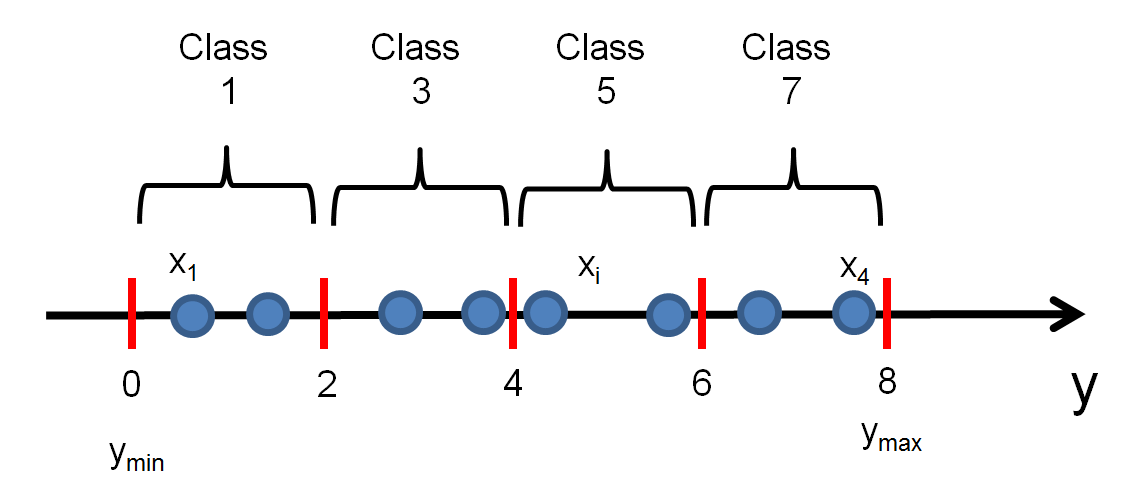
\includegraphics[width=0.5\linewidth]{images/Discretize_binning}
%%	\caption{Example of discretization by binning a continuous label $y$ into $Q=4$ equal-length intervals. Each interval is associated to a unique class label. In this example, the class label for each interval is equal to the mean in each interval.}
%%	\label{fig:Discretize_binning}
%%\end{figure}
%This approach may leads to border effects between the classes. For instance, two samples $\textbf{x}_i$ and $\textbf{x}_j$ that are close to a frontier and that are on different sides of the border will be considered as different. Moreover, a new sample $\textbf{x}_j$ will have its labels $y_j$ assigned to a class and not a real continuous value. \\
%%\begin{figure}[h!]
%%	\centering
%%	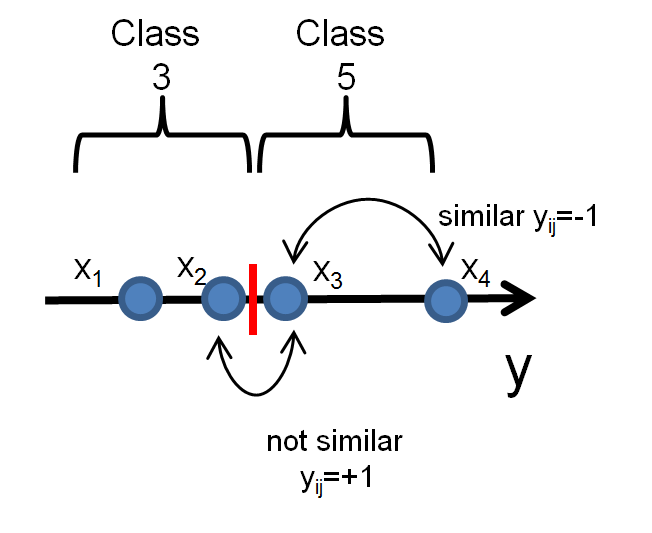
\includegraphics[width=0.4\linewidth]{images/Discretize_binning_border_effect}
%%	\caption{Border effect problems. In this example, $\textbf{x}_2$ and $\textbf{x}_3$ have closer value labels $y_2$ and $y_3$ than $\textbf{x}_3$ and $\textbf{x}_4$. However, with the discretization $\textbf{x}_2$ and $\textbf{x}_3$ don't belong to the same class and thus are consider as not similar.}
%%	\label{fig:Discretize_binning_border_effect}
%%\end{figure}
%The second approach considers the continuous value of $y_i$, computes the absolute difference $|y_i-y_j|$ between the labels $y_i$ and $y_j$, and compare this value to a threshold $\epsilon$. Geometrically, a tube of size $\epsilon$ around each value of $y_i$ is built. Two samples $\textbf{x}_i$ and  $\textbf{x}_j$ are considered as similar if the absolute difference $|y_i-y_j|$ is lower than $\epsilon$ (Fig. \ref{fig:pairwise_label_tube}):
%\begin{equation}
%y_{ij} = 
%\left\{
%\begin{split}
%\begin{aligned}
%-1 & \text{\quad if } |y_i-y_j| \leq \epsilon \\ 
%+1 & \text{\quad otherwise }
%\end{aligned} 
%\end{split}
%\right.
%\end{equation}
%
%\begin{figure}[h!]
%	\centering
%	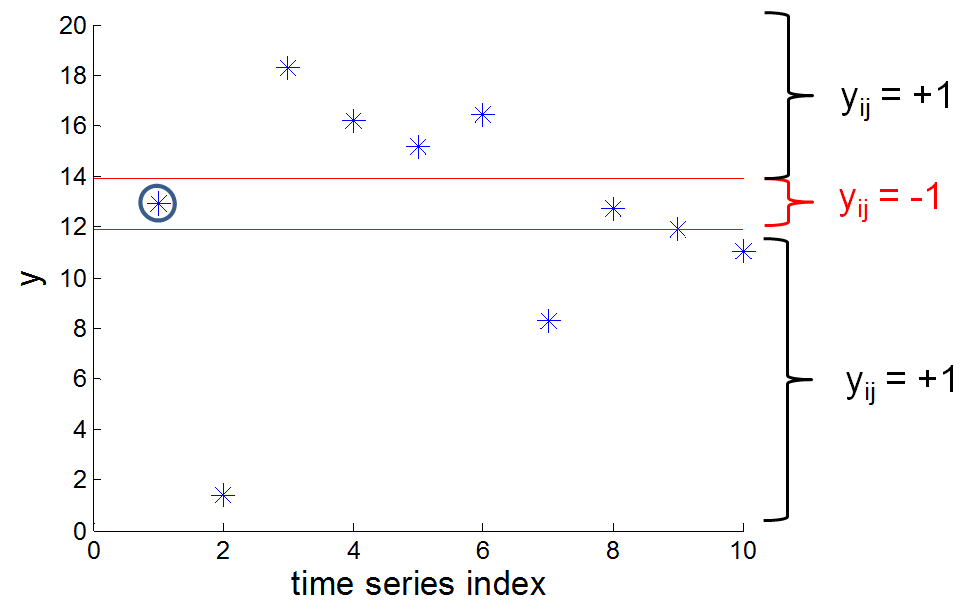
\includegraphics[width=0.65\linewidth]{images/pairwise_label_tube}
%	\caption{Example of pairwise label definition using an $\epsilon$-tube (red lines) around the time series $\textbf{x}_i$ (circled in blue). For, time series $\textbf{x}_j$ that falls into the tube, the pairwise label is $y_{ij} = -1$ (similar) and outside of the tube, $y_{ij} = +1$ (not similar).}
%	\label{fig:pairwise_label_tube}
%\end{figure}


%\section{Geometric interpretation}
%\todo[inline]{A changer avec les retours de Sylvain. Michèle pense que l'état, cette section est dure à comprendre. D'après Michèle, il faut 1) soit prendre + de place pour expliquer la signification géométrique 2) ou soit ne pas mettre cette partie car étant compliquée, cela pourrait nuire au lecteur. Qu'en penses tu Ahlame?}
%In this section, we give a geometric understanding of the differences between {\sc lp}/{\sc qp} resolution (left) and \textsc{svm}-based resolution (right). Fig. \ref{fig:Linear} shows the Linear Programming ({\sc lp}) and \textsc{svm} resolutions of a $k$-NN problem with $k=2$ neighborhoods. \\
%
%For {\sc lp}, the problem is solved for each neighborhood (blue and red) independently as shown in Fig. \ref{fig:LP_separate}. We recall that {\sc lp}/{\sc qp} resolutions, support vectors are triplets of time series made of a target pair $\textbf{x}_{ij}$ and a pair of different classes $\textbf{x}_{il}$ (black arrows). Support vectors represent triplet which resulting distance $D(\textbf{x}_{ij}, \textbf{x}_{il})$ are the lowest. The optimization problem tends to maximize the margin between these triplets. The global solution (Fig. \ref{fig:Linear} (left)) is a compromise of all of the considered margins. In this case, the global margin is equal to one of the local margin. Note that the global {\sc lp} solution is not always the same as the best local solution. For \textsc{svm}-based resolution (Fig. \ref{fig:Linear} (right)), the problem involves all pairs and the margin is optimized so that pairs $\textbf{x}_{ij}$ and $\textbf{x}_{il}$ are globally separated.
%
%
%
%\begin{figure}[h!]
%	\centering
%	\begin{minipage}[b]{1\linewidth}
%		\centerline{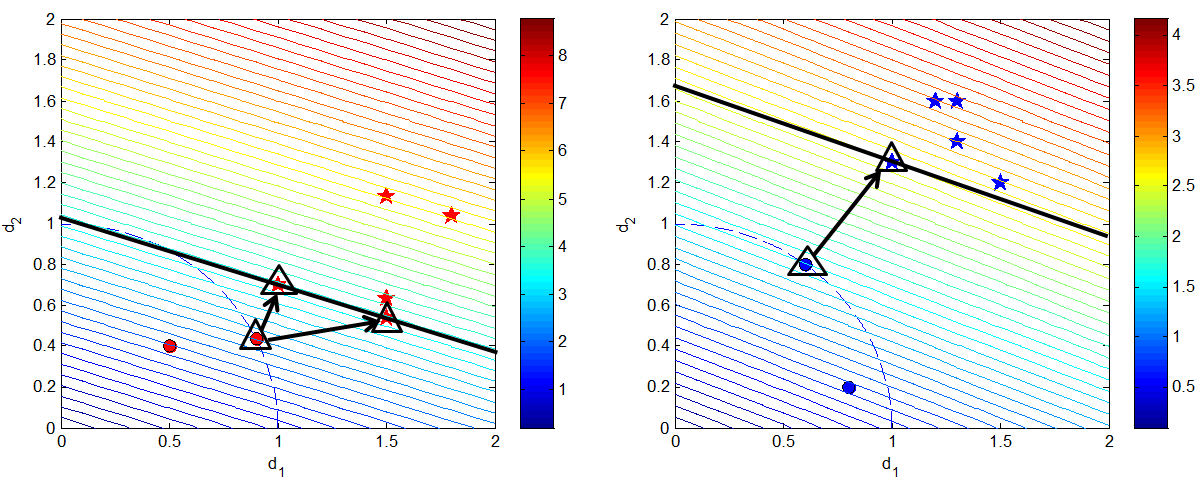
\includegraphics[width=1\linewidth]{images/InterpretationLP}}
%	\end{minipage}
%	\caption{Solutions found by solving the {\sc lp} problem for $k=2$ neighborhood. Positive pairs (different classes) are indicated in stars and negative pairs (target pairs) are indicated in circle. Red and blue lines shows the margin when solving the problem for each neighborhood (red and blue points) separately. Support vector are indicated in black triangles: in the red neighborhood (left), 2 support vectors are retained and in the blue neighborhood (right), only one support vector is necessary.}
%	\label{fig:LP_separate}
%\end{figure}
%
%\begin{figure}[h!]
%	\centering
%	\begin{minipage}[b]{1\linewidth}
%		\centerline{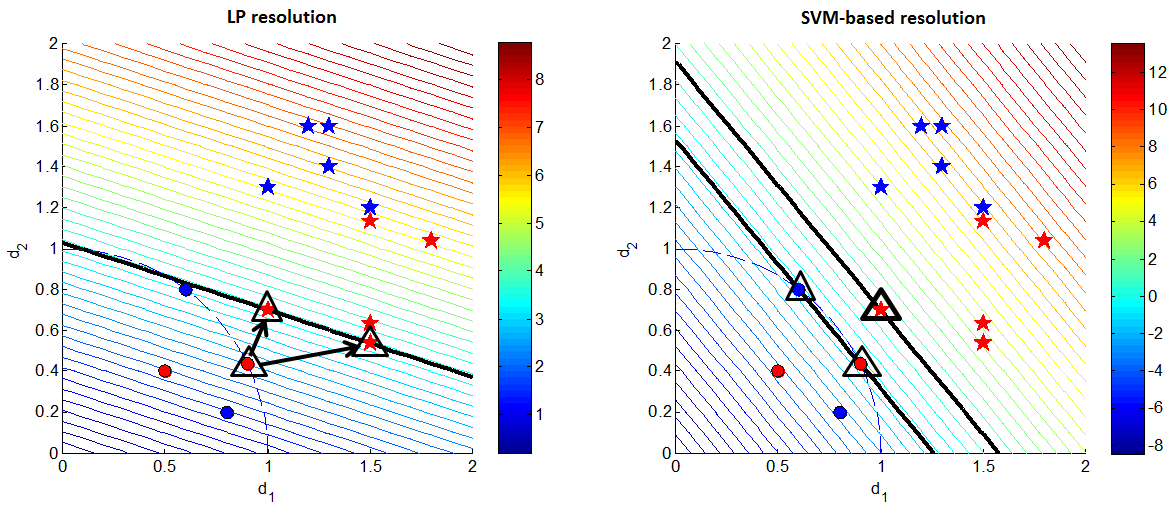
\includegraphics[width=1\linewidth]{images/InterpretationLP_SVM}}
%	\end{minipage}
%	\caption{Solutions found by solving the {\sc lp} problem (left) and the \textsc{svm} problem (right). The global margin is indicated in black and the metric is represented in color levels. Support vectors made of triplets are indicated in black triangles. For the \textsc{svm}, the black lines indicates the \textsc{svm} canonical hyperplane where the support vector lies (black triangles).}
%	\label{fig:Linear}
%\end{figure}

\newpage
\section{Conclusion}
To learn a multi-modal and multi-scale temporal combined metric, we propose in this chapter to embed time series into a dissimilarity space. The multi-modal and multi-scale metric learning (\textsc{m$^2$tml}) problem can be formalized as a problem of learning a function in the dissimilarity space, that ensures the properties of a dissimilarity. We formulate the \textsc{m$^2$tml} problem into a general optimization problem involving a pull and push term. Choosing a $m$-neighborhood, greater than the $k$-neighborhood allows to generalize better the learnt metric. From the general formalization, we propose three different formalizations (Linear, Quadratic, \textsc{svm}-based). Table \ref{tab:resume_methode} sums up the characteristics of each formalization and the induced dissimilarity.

\begin{table}[h!]
	\small
	\centering
	\renewcommand{\arraystretch}{0.85}
	\resizebox{0.7\textwidth}{!}{
		\setlength{\tabcolsep}{1pt}
		\begin{tabular}{lccc}
			\hline
			& Linear		& Quadratic 	& SVM-based\\
			& formalization & formalization & formalization\\
			\hline
			$D$  					& Linear & Linear/Non-linear & Linear/Non-linear \\
			Sparcity 				& Yes	& No    & Yes/No 	\\
			Dissimilarity properties& Yes 	& No (non-positivity) & Yes		\\
			\hline
		\end{tabular}}
		\caption{The different formalizations for \textsc{m$^2$tml}}
		\label{tab:resume_methode}
	\end{table}

\noindent The adaptation of \textsc{svm} in the dissimilarity space to learn the multi-modal and multi-scale metric $D$ have brought us to propose a pre-processing step before solving the problem such as the neighborhood scaling, and a post-processing step such as defining the metric $D$.

As we have defined all functions components of our algorithms (learning, testing), we test our proposed algorithms {\sc m}$^2${\sc tml} in the next chapter on large public datasets. 



%\newpage
%\section{Problem 2}
%\todo[inline]{ancienne proposition. Il peut y avoir des problèmes dans l'inversibilité de la matrice}
%%\begin{itemize}
%%	\item Passer de la forme LP (forme primale) et par transformation, arriver à la forme duale
%%	\item Montrer les similitudes avec la résolution \textsc{svm}
%%	\item Montrer que l'on peut kerneliser la méthode
%%\end{itemize}
%The primal formulation supposed that the metric $D$ is a linear combination of the metrics $d_h$. The primal formulation being similar to the one of \textsc{svm}, it can be derived into its dual form to obtain non-linear solutions for $D$.
%% Similarly to the SVM dual formulation (Section \ref{sec:dualSVM}), the TML primal formulation in Eq. \ref{eq:MMLPrimal} can be derived into its dual form to obtain non-linear solutions for $D$. 
%For that, we consider in the objective function (Eq. \ref{eq:MMLPrimal}), the square of the $L_2$-norm on $\textbf{w}$ as the regularizer term, $\frac{1}{2}||\textbf{X}_{pull}^T \textbf{w}||_2^2$:
%
%\begin{align}
%	&\displaystyle 		\argmin_{\textbf{w},\xi}
%	\left\lbrace \frac{1}{2}||\textbf{X}_{pull}^T \textbf{w}||_2^2						
%	+					
%	C\sum\limits_{i,j \rightsquigarrow i,l} \frac{1+y_{il}}{2}.\xi_{ijl}
%	\right\rbrace  \label{eq:MMLPrimalL2} \\
%	&\text{s.t.  } \forall j \rightsquigarrow i, y_l\neq y_i, \nonumber \\
%	& \qquad \textbf{w}^T(\textbf{x}_{il}-\textbf{x}_{ij}) \geq 1-\xi_{ijl} \label{eq:MMLPrimalL2_constraints1} \\
%	& \qquad \xi_{ijl} \geq 0 \label{eq:MMLPrimalL2_constraints2}
%\end{align}
%This formulation can be reduced to the minimization of the following Lagrange function $L(\textbf{w},\xi,\boldsymbol{\alpha},\textbf{r})$, consisting of the sum of the objective function (Eq. \ref{eq:MMLPrimalL2}) and the constraints (Eqs. \ref{eq:MMLPrimalL2_constraints1} and \ref{eq:MMLPrimalL2_constraints2}) multiplied by their respective Lagrange multipliers $\boldsymbol{\alpha}$ and $\textbf{r}$:
%\begin{equation}
%\begin{aligned}
%L(\textbf{w},\xi,\boldsymbol{\alpha},\textbf{r}) 
%= & 
%\frac{1}{2}||\textbf{X}_{pull}^T \textbf{w}||_2^2
%+ C \sum\limits_{ijl} \frac{1+y_{il}}{2} \xi_{ijl} - \sum\limits_{ijl}r_{ijl} \xi_{ijl} \\
%&  - \sum\limits_{ijl} \alpha_{ijl}\left( \textbf{w}^T(\textbf{x}_{il}-\textbf{x}_{ij}-1+\xi_{ijl} \right))
%\label{eq:OptimizationDual}
%\end{aligned}
%\end{equation}
%\noindent where $\alpha_{ijl} \geq 0$ and $r_{ijl} \geq 0$ are the Lagrange multipliers. At the minimum value of $L(\textbf{w},\xi,\boldsymbol{\alpha},\textbf{r})$, we assume the derivatives with respect to $\textbf{w}$ and $\xi_{ijl}$ are set to zero:
%\begin{align*}
%	\frac{\partial L}{\partial \textbf{w}} 
%	& = 
%	\textbf{X}_{pull}^T \textbf{X}_{pull} \textbf{w} 
%	- \sum\limits_{ijl} \alpha_{ijl}(\textbf{x}_{il}-\textbf{x}_{ij}) 
%	= 0 \\
%	\frac{\partial L}{\partial \xi_{ijl}} & = C - \alpha_{ijl} - r_{ijl} = 0
%\end{align*}
%\noindent that leads to:
%\begin{align}
%	& \textbf{w} = (\textbf{X}_{pull} \textbf{X}_{pull}^T)^{-1}  
%	\sum\limits_{ijl} \alpha_{ijl}(\textbf{x}_{il}-\textbf{x}_{ij}) \label{Eq:eqn_w} 
%	\\ 
%	& r_{ijl} = C - \alpha_{ijl} \label{Eq:eqn_w2}
%\end{align}
%
%\noindent Substituting Eq. \ref{Eq:eqn_w} and \ref{Eq:eqn_w2} back into $L(\textbf{w},\xi,\boldsymbol{\alpha},\textbf{r})$ in Eq. \ref{eq:OptimizationDual}, we get the dual formulation\footnote{complete details of the calculations in Appendix \ref{chap:app:qp_resolution}}:
%\begin{align}
%	&\displaystyle \argmax_{\boldsymbol{\alpha}} \left\lbrace 
%	\sum\limits_{ijl} \alpha_{ijl} 
%	- \frac{1}{2} \sum\limits_{ijl} \sum\limits_{i'j'l'}
%	\alpha_{ijl} \alpha_{i'j'l'}
%	(\textbf{x}_{il}-\textbf{x}_{ij})^T
%	(\textbf{X}_{pull} \textbf{X}_{pull}^T)^{-1}
%	(\textbf{x}_{i'l'}-\textbf{x}_{i'j'}) \right\rbrace \label{eq:OptimDual} \\
%	&\text{s.t. $\forall$ $i$, $j \rightsquigarrow i$ and $l$ s.t. $y_{il}=+1$:} \nonumber \\
%	& 0 \leq \alpha_{ijl} \leq C
%	\label{eq:OptimDualconstraint}
%\end{align}
%
%\noindent For any new pair of samples $\textbf{x}_{i'}$ and $\textbf{x}_{j'}$, the resulting metric $D$ writes: 
%\begin{align}
%	D(\textbf{x}_{i'j'}) = & \textbf{w}^T \textbf{x}_{i'j'} \label{eq:D1} \\
%	D(\textbf{x}_{i'j'}) = & \sum\limits_{ijl} \alpha_{ijl} 
%	(\textbf{x}_{il}-\textbf{x}_{ij})^T
%	(\textbf{X}_{pull}\textbf{X}_{pull}^T)^{-1}
%	\textbf{x}_{i'j'}
%	\label{eq:D1_2}
%\end{align}
%% At the optimality, only the triplet $(\textbf{x}_{il}-\textbf{x}_{ij})$ which $\textbf{x}_{il}$ that has the $L_2$ norm greater than 1 and that lies closest to the unit circle of targets $\textbf{x}_{ij}$ or those triplets that have a $L_2$ norm lower that one, have $\alpha_{ijl} > 0$. These points are the support vectors. 
%with $\textbf{w}$ defined in Eq. \ref{Eq:eqn_w}. At the optimality, only the triplets $(\textbf{x}_{il}-\textbf{x}_{ij})$ with $\alpha_{ijl} > 0$ are considered as the support vectors. The direction $\textbf{w}$ of the metric $D$ is lead by these triplets. All other triplets have $\alpha_{ijl} = 0$ (non-support vector), and the metric $D$ is independent from this triplets. If we remove some of the non-support vectors, the metric $D$ remains unaffected. From the viewpoint of optimization theory, we can also see this from the Karush-Kuhn-Tucker (KKT) conditions: the complete set of conditions which must be satisfied at the optimum of a constrained optimization problem. At the optimum, the Karush-Kuhn-Tucker (KKT) conditions apply, in particular:
%\begin{equation*}
%	\alpha_{ijl} (\textbf{w}^T (\textbf{x}_{il}-\textbf{x}_{ij}) - 1 + \xi_{ijl}) = 0
%\end{equation*}
%
%\noindent from which we deduce that either $\textbf{w}^T(\textbf{x}_{il}-\textbf{x}_{ij}) > 1 $ and $\alpha_{ijl} = 0$ (the triplet $(\textbf{x}_{il}-\textbf{x}_{ij})$ is a non-support vector), or $\textbf{w}^T(\textbf{x}_{il}-\textbf{x}_{ij}) = 1- \xi_{ijl}$ and $\alpha_{ijl} > 0$ (the triplet is a support vector). Therefore, the learned metric $D$ is a combination of scalar products between new pairs $\textbf{x}_{i'j'}$ and a few number of triplets $\textbf{x}_{ijl}$ of the training set. \\
%
%
%\noindent \textbf{Extension to non-linear function of $D$} \\
%\noindent The above formula can extended to non-linear function for the metric $D$. The dual formulation in Eq.~\ref{eq:OptimDual} only relies on the inner product $(\textbf{x}_{i'l'}-\textbf{x}_{i'j'})^T (\textbf{X}_{pull} \textbf{X}_{pull}^T)^{-1} (\textbf{x}_{il}-\textbf{x}_{ij})$. We can hence apply the kernel trick on Eqs. \ref{eq:D1} and \ref{eq:D1_2} to find non-linear solutions for $D$:
%\begin{align}
%	D(\textbf{x}_{i'j'}) & = \textbf{w}^T \phi(\textbf{x}_{i'j'}) \nonumber\\
%	D(\textbf{x}_{i'j'}) &= \sum\limits_{ijl} \alpha_{ijl} 
%	\phi(
%	\textbf{x}_{il}-\textbf{x}_{ij}
%	)
%	\phi(	
%	\textbf{x}_{i'j'}
%	) \nonumber \\
%	D(\textbf{x}_{i'j'}) &= \sum\limits_{ijl} \alpha_{ijl} 
%	K(\textbf{x}_{il}-\textbf{x}_{ij} ; \textbf{x}_{i'j'}) \nonumber				
%\end{align}
%These equations suppose that the null vector $\textbf{0}$ in the original space is transformed through the transformation $\phi$ into the null vector: $\phi(\textbf{0})=\textbf{0}$ in the feature space. We recall that $D(\textbf{x}_{ii} = \textbf{0})$ is expected to be equal to zero (distinguishability property in Section \ref{sec:property_metric}). However, if the vectors $\textbf{x}_{ij}$ are projected in a feature space by a transformation $\phi$, it doesn't guarantee that $\phi(\textbf{0})=\textbf{0}$. Fig. \ref{fig:Kernel_nonHomogene} illustrates the idea for a polynomial kernel in which $\phi(\textbf{0}) = [0, 0, 0, 1]^T$. Thus, the metric measure needs to be computed in the feature space relatively to the projection of $\phi(\textbf{0})$. This is done by adding a term $\textbf{w}^T \phi(\textbf{0})$ to Eqs. \ref{eq:D1} and \ref{eq:D1_2}:
%
%\begin{align}
%	D(\textbf{x}_{i'j'}) & = \textbf{w}^T \phi(\textbf{x}_{i'j'}) - \textbf{w}^T \phi(\textbf{0})\\
%	D(\textbf{x}_{i'j'}) &= \sum\limits_{ijl} \alpha_{ijl} 
%	\phi(
%	\textbf{x}_{il}-\textbf{x}_{ij}
%	)
%	\phi(	
%	\textbf{x}_{i'j'}-\textbf{x}_{ij}
%	) 
%	-
%	\sum\limits_{ijl} \alpha_{ijl} 
%	\phi(
%	\textbf{x}_{il}-\textbf{x}_{ij}
%	)
%	\phi(	
%	\textbf{0}-\textbf{x}_{ij}
%	) 				
%	\\
%	D(\textbf{x}_{i'j'}) &= \sum\limits_{ijl} \alpha_{ijl} 
%	K
%	\left( 
%	\textbf{x}_{il}-\textbf{x}_{ij}
%	;	
%	\textbf{x}_{i'j'}-\textbf{x}_{ij}
%	\right) 		
%	-
%	\sum\limits_{ijl} \alpha_{ijl} 
%	K
%	\left( 
%	\textbf{x}_{il}-\textbf{x}_{ij}
%	;	
%	\textbf{0}-\textbf{x}_{ij}
%	\right) 		
%	\label{Eq:nonlinearD}		
%\end{align}
%%For any new pair of samples $\textbf{x}_{i'}$ and $\textbf{x}_{j'}$, the resulting metric $D$ writes: 
%%\begin{align}
%%D(\textbf{x}_{i'j'}) = & \textbf{w}^T \textbf{x}_{i'j'} - \textbf{w}^T \textbf{0} 
%%\nonumber \\
%%D(\textbf{x}_{i'j'}) = & \sum\limits_{ijl} \alpha_{ijl} 
%%(\textbf{x}_{il}-\textbf{x}_{ij})^T
%%(\textbf{X}_{pull}\textbf{X}_{pull}^T)^{-1}
%%\textbf{x}_{i'j'} 
%%-
%%\sum\limits_{ijl} \alpha_{ijl} 
%%(\textbf{x}_{il}-\textbf{x}_{ij})^T
%%(\textbf{X}_{pull}\textbf{X}_{pull}^T)^{-1}
%%\textbf{0}
%%\nonumber \\
%%& -\sum\limits_{ijl} \alpha_{ijl} 
%%(\textbf{x}_{il}-\textbf{x}_{ij})^T
%%(\textbf{X}_{pull}\textbf{X}_{pull}^T)^{-1}\textbf{x}_{ij} + \sum\limits_{ijl} \alpha_{ijl} 
%%(\textbf{x}_{il}-\textbf{x}_{ij})^T
%%(\textbf{X}_{pull}\textbf{X}_{pull}^T)^{-1}\textbf{x}_{ij}
%%\nonumber \\
%%D(\textbf{x}_{i'j'}) = & \sum\limits_{ijl} \alpha_{ijl} 
%%(\textbf{x}_{il}-\textbf{x}_{ij})^T
%%(\textbf{X}_{pull}\textbf{X}_{pull}^T)^{-1}
%%(\textbf{x}_{i'j'}-\textbf{x}_{ij}) 
%%\nonumber \\
%%& - \sum\limits_{ijl} \alpha_{ijl} 
%%(\textbf{x}_{il}-\textbf{x}_{ij})^T
%%(\textbf{X}_{pull}\textbf{X}_{pull}^T)^{-1}
%%(\textbf{0}-\textbf{x}_{ij}) \label{eq:D2}
%%\end{align}
%\noindent where $\textbf{0}$ denotes the null vector. The resulting metric $D$ is made of two terms. The first one, $\textbf{w}^T \phi(\textbf{x}_{i'j'})$, is the metric measure for a new pair $\textbf{x}_{i'j'}$. The second term, $\textbf{w}^T \phi(\textbf{0})$, adapts the metric measure relatively to the origin point. 
%
%\begin{figure}[h!]
%	\centering
%	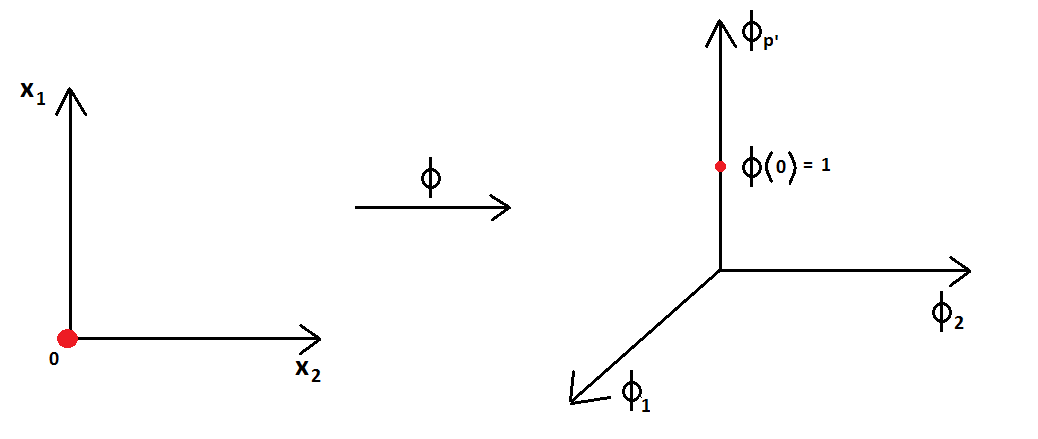
\includegraphics[width=0.9\linewidth]{images/Kernel_nonHomogene}
%	\caption{Illustration of samples in $\mathbb{R}^2$. The transformation $\phi$ for a polynomial kernel $K(\textbf{x}_i,\textbf{x}_j)=(\textbf{x}_i^T \textbf{x}_j + c)^d$ with $c=1$ and $d=2$ can be written explicitly: $\phi(\textbf{x}_i)= [x_{i1}^2, x_{i2}^2, \sqrt{2} x_{i1} x_{i2}, 1]^T$. The origin point $\textbf{x}_i=[0,0]^T$ is projected in the Hilbert space as $\phi(\textbf{x}_i=\textbf{0}) = [0, 0, 0, 1]^T$.}
%	\label{fig:Kernel_nonHomogene}
%\end{figure}
%
%However, to define proper metrics that respects the properties of metrics (Section \ref{sec:property_metric}), specific kernels must be used. Our work don't propose any solutions to this problem but open the field for new research on this topic. 
%
%
%\section{Problem 3}
%%\begin{itemize}
%%	\item Passer de la forme LP (forme primale) et par transformation, arriver à la forme duale
%%	\item Montrer les similitudes avec la résolution \textsc{svm}
%%	\item Montrer que l'on peut kerneliser la méthode
%%\end{itemize}
%
%\todo[inline]{Nouvelle proposition qui change la régularisation et permet de ne plus obtenir de problème d'inversibilité de la matrice}
%
%The formulation in Eq. \ref{eq:MMLPrimal} suppose that the metric $D$ is a linear combination of the metrics $d_h$. The primal formulation being similar to the one of \textsc{svm}, it can be derived into its dual form to obtain non-linear solutions for $D$.
%
%\noindent Let $\textbf{X}_{tar}$ be a $(m.n) \times p$ matrix containing the pairwise vector $\textbf{x}_{ij} \in Pull_i$. Let $\textbf{M} = Diag(\textbf{X}_{tar}^T\textbf{X}_{tar}):$
%\begin{equation}
%	\textbf{M} = Diag(\textbf{X}_{tar}^T\textbf{X}_{tar}) = 
%	\begin{bmatrix} 
%		\sum\limits_{\substack{i \\ j \in Pull_i}} d_1^2(\textbf{x}_{ij}) 		&  	& 0 \\ 
%			& \ddots 	&  \\ 
%		0 		&  	& \sum\limits_{\substack{i \\ j \in Pull_i}} d_p^2(\textbf{x}_{ij})
%		\end{bmatrix}
%\end{equation}
%% Similarly to the SVM dual formulation (Section \ref{sec:dualSVM}), the TML primal formulation in Eq. \ref{eq:MMLPrimal} can be derived into its dual form to obtain non-linear solutions for $D$. 
%
%\noindent Then, we change the regularizer in the objective function of Eq. \ref{eq:MMLPrimal}:
%\begin{equation}
%	R(w) = \frac{1}{2} \textbf{w}^T \textbf{M} \textbf{w} = \frac{1}{2} \sum\limits_{h=1}^{p} \sum\limits_{\substack{i \\ j \in Pull_i}} w_h^2 d_h^2(\textbf{x}_{ij})
%\end{equation}
%\noindent From this, the optimization problem becomes:
%\begin{align}
%	&\displaystyle 		\argmin_{\textbf{w},\xi}
%	\left\lbrace \frac{1}{2} \textbf{w}^T \textbf{M} \textbf{w}					
%	+					
%	C\sum\limits_{i,j \rightsquigarrow i,l} \frac{1+y_{il}}{2} \xi_{ijl}
%	\right\rbrace  \label{eq:MMLPrimalL2} \\
%	&\text{s.t.  } \forall j \rightsquigarrow i, l, \nonumber \\
%	& \qquad \textbf{w}^T(\textbf{x}_{il}-\textbf{x}_{ij}) \geq 1-\xi_{ijl} \label{eq:MMLPrimalL2_constraints1} \\
%	& \qquad \xi_{ijl} \geq 0 \label{eq:MMLPrimalL2_constraints2}
%\end{align}
%This formulation can be reduced to the minimization of the following Lagrange function $L(\textbf{w},\xi,\boldsymbol{\alpha},\textbf{r})$, consisting of the sum of the objective function (Eq. \ref{eq:MMLPrimalL2}) and the constraints (Eqs. \ref{eq:MMLPrimalL2_constraints1} and \ref{eq:MMLPrimalL2_constraints2}) multiplied by their respective Lagrange multipliers $\boldsymbol{\alpha}$ and $\textbf{r}$:
%\begin{equation}
%\begin{aligned}
%	L(\textbf{w},\xi,\boldsymbol{\alpha},\textbf{r}) 
%	= & 
%	\frac{1}{2} \textbf{w}^T \textbf{M} \textbf{w}
%	+ C \sum\limits_{ijl} \frac{1+y_{il}}{2} \xi_{ijl} - \sum\limits_{ijl}r_{ijl} \xi_{ijl} \\
%	&  - \sum\limits_{ijl} \alpha_{ijl}\left( \textbf{w}^T(\textbf{x}_{il}-\textbf{x}_{ij}-1+\xi_{ijl} \right))
%	\label{eq:OptimizationDual}
%\end{aligned}
%\end{equation}
%\noindent where $\alpha_{ijl} \geq 0$ and $r_{ijl} \geq 0$ are the Lagrange multipliers. At the minimum value of $L(\textbf{w},\xi,\boldsymbol{\alpha},\textbf{r})$, we assume the derivatives with respect to $\textbf{w}$ and $\xi_{ijl}$ are set to zero:
%
%\begin{align*}
%\frac{\partial L}{\partial \textbf{w}} 
%& = 
%\textbf{M} \textbf{w} 
%- \sum\limits_{ijl} \alpha_{ijl}(\textbf{x}_{il}-\textbf{x}_{ij}) 
%= 0 \\
%\frac{\partial L}{\partial \xi_{ijl}} & = C - \alpha_{ijl} - r_{ijl} = 0
%\end{align*}
%\noindent The matrix $\textbf{M}$ being diagonale, it is thus inversible. The equations leads to:
%\begin{align}
%& \textbf{w} = \textbf{M}^{-1}  
%\sum\limits_{ijl} \alpha_{ijl}(\textbf{x}_{il}-\textbf{x}_{ij}) \label{Eq:eqn_w} 
%\\ 
%& r_{ijl} = C - \alpha_{ijl} \label{Eq:eqn_w2}
%\end{align}
%
%\noindent Substituting Eq. \ref{Eq:eqn_w} and \ref{Eq:eqn_w2} back into $L(\textbf{w},\xi,\boldsymbol{\alpha},\textbf{r})$ in Eq. \ref{eq:OptimizationDual}, we get the {\sc mld} dual formulation\footnote{complete details of the calculations in Appendix \ref{chap:app:qp_resolution}}:
%
%\begin{align}
%&\displaystyle \argmax_{\boldsymbol{\alpha}} \left\lbrace 
%\sum\limits_{ijl} \alpha_{ijl} 
%- \frac{1}{2} \sum\limits_{ijl} \sum\limits_{i'j'l'}
%\alpha_{ijl} \alpha_{i'j'l'}
%(\textbf{x}_{il}-\textbf{x}_{ij})^T
%\textbf{M}^{-1}
%(\textbf{x}_{i'l'}-\textbf{x}_{i'j'}) \right\rbrace \label{eq:OptimDual} \\
%&\text{s.t. $\forall$ $i$, $j \rightsquigarrow i$ and $l$ s.t. $y_{il}=+1$:} \nonumber \\
%& 0 \leq \alpha_{ijl} \leq C
%\label{eq:OptimDualconstraint}
%\end{align}
%
%\noindent For any new pair of samples $\textbf{x}_{i'}$ and $\textbf{x}_{j'}$, the resulting metric $D$ writes: 
%\begin{align}
%D(\textbf{x}_{i'j'}) = & \textbf{w}^T \textbf{x}_{i'j'} \label{eq:D1} \\
%D(\textbf{x}_{i'j'}) = & \sum\limits_{ijl} \alpha_{ijl} 
%(\textbf{x}_{il}-\textbf{x}_{ij})^T
%\textbf{M}^{-1}
%\textbf{x}_{i'j'}
%\label{eq:D1_2}
%\end{align}
%% At the optimality, only the triplet $(\textbf{x}_{il}-\textbf{x}_{ij})$ which $\textbf{x}_{il}$ that has the $L_2$ norm greater than 1 and that lies closest to the unit circle of targets $\textbf{x}_{ij}$ or those triplets that have a $L_2$ norm lower that one, have $\alpha_{ijl} > 0$. These points are the support vectors. 
%with $\textbf{w}$ defined in Eq. \ref{Eq:eqn_w}. At the optimality, only the triplets $(\textbf{x}_{il}-\textbf{x}_{ij})$ with $\alpha_{ijl} > 0$ are considered as the support vectors. The direction $\textbf{w}$ of the metric $D$ is lead by these triplets. All other triplets have $\alpha_{ijl} = 0$ (non-support v ector), and the metric $D$ is independent from this triplets. If we remove some of the non-support vectors, the metric $D$ remains unaffected. From the viewpoint of optimization theory, we can also see this from the Karush-Kuhn-Tucker (KKT) conditions: the complete set of conditions which must be satisfied at the optimum of a constrained optimization problem. At the optimum, the Karush-Kuhn-Tucker (KKT) conditions apply, in particular:
%\begin{equation*}
%\alpha_{ijl} (\textbf{w}^T (\textbf{x}_{il}-\textbf{x}_{ij}) - 1 + \xi_{ijl}) = 0
%\end{equation*}
%
%\noindent from which we deduce that either $\textbf{w}^T(\textbf{x}_{il}-\textbf{x}_{ij}) > 1 $ and $\alpha_{ijl} = 0$ (the triplet $(\textbf{x}_{il}-\textbf{x}_{ij})$ is a non-support vector), or $\textbf{w}^T(\textbf{x}_{il}-\textbf{x}_{ij}) = 1- \xi_{ijl}$ and $\alpha_{ijl} > 0$ (the triplet is a support vector). Therefore, the learned metric $D$ is a combination of scalar products between new pairs $\textbf{x}_{i'j'}$ and a few number of triplets $\textbf{x}_{ijl}$ of the training set. \\
%
%
%\noindent \textbf{Extension to non-linear function of $D$} \\
%\noindent The above formula can extended to non-linear function for the metric $D$. The dual formulation in Eq.~\ref{eq:OptimDual} only relies on the inner product $(\textbf{x}_{i'l'}-\textbf{x}_{i'j'})^T \textbf{M}^{-1} (\textbf{x}_{il}-\textbf{x}_{ij})$. We can hence apply the kernel trick on Eqs. \ref{eq:D1} and \ref{eq:D1_2} to find non-linear solutions for $D$. As $\textbf{M}^{-1}$ is a diagonal matrix, it is inversible and can be written $\textbf{M}^{-1} = \textbf{M}^{-\frac{1}{2}} \textbf{M}^{-\frac{1}{2}}$. Thus:
%\begin{align}
%		(\textbf{x}_{i'l'}-\textbf{x}_{i'j'})^T \textbf{M}^{-1} (\textbf{x}_{il}-\textbf{x}_{ij}) 
%		& = (\textbf{x}_{i'l'}-\textbf{x}_{i'j'})^T \textbf{M}^{-\frac{1}{2}} \textbf{M}^{-\frac{1}{2}} (\textbf{x}_{il}-\textbf{x}_{ij})	\nonumber	\\
%		& = \left( \textbf{M}^{-\frac{1}{2}} (\textbf{x}_{i'l'}-\textbf{x}_{i'j'}) \right)^T \left( \textbf{M}^{-\frac{1}{2}} (\textbf{x}_{il}-\textbf{x}_{ij}) \right) \nonumber \\
%		& = <\textbf{M}^{-\frac{1}{2}} (\textbf{x}_{i'l'}-\textbf{x}_{i'j'}) ; \textbf{M}^{-\frac{1}{2}} (\textbf{x}_{il}-\textbf{x}_{ij}) > \nonumber \\
%		& = K(\textbf{M}^{-\frac{1}{2}} (\textbf{x}_{i'l'}-\textbf{x}_{i'j'}) ;  \textbf{M}^{-\frac{1}{2}} (\textbf{x}_{il}-\textbf{x}_{ij}) ) \nonumber
%\end{align}
%\noindent By replacing the inner product by a kernel back into Eqs. \ref{eq:D1} \& \ref{eq:D1_2}, we obtain:
%\begin{align}
%D(\textbf{x}_{i'j'}) & = \textbf{w}^T \phi(\textbf{M}^{-\frac{1}{2}}\textbf{x}_{i'j'}) \nonumber\\
%D(\textbf{x}_{i'j'}) &= \sum\limits_{ijl} \alpha_{ijl} 
%\phi( \textbf{M}^{-\frac{1}{2}}
%(\textbf{x}_{il}-\textbf{x}_{ij})
%)
%\phi(	
%\textbf{M}^{-\frac{1}{2}} \textbf{x}_{i'j'}
%) \nonumber \\
%D(\textbf{x}_{i'j'}) &= \sum\limits_{ijl} \alpha_{ijl} 
%K(\textbf{M}^{-\frac{1}{2}} (\textbf{x}_{il}-\textbf{x}_{ij}) ; \textbf{M}^{-\frac{1}{2}}\textbf{x}_{i'j'}) \nonumber				
%\end{align}
%These equations suppose that the null vector $\textbf{0}$ in the original space is transformed through the transformation $\phi$ into the null vector: $\phi(\textbf{0})=\textbf{0}$ in the feature space. We recall that $D(\textbf{x}_{ii} = \textbf{0})$ is expected to be equal to zero (distinguishability property in Section \ref{sec:property_metric}). However, if the vectors $\textbf{x}_{ij}$ are projected in a feature space by a transformation $\phi$, it doesn't guarantee that $\phi(\textbf{0})=\textbf{0}$. Fig. \ref{fig:Kernel_nonHomogene} illustrates the idea for a polynomial kernel in which $\phi(\textbf{0}) = [0, 0, 0, 1]^T$. Thus, the metric measure needs to be computed in the feature space relatively to the projection of $\phi(\textbf{0})$. This is done by adding a term $\textbf{w}^T \phi(\textbf{0})$ to Eqs. \ref{eq:D1} and \ref{eq:D1_2}:
%\begin{align}
%D(\textbf{x}_{i'j'}) & = \textbf{w}^T \phi(\textbf{M}^{-\frac{1}{2}}\textbf{x}_{i'j'}) - \textbf{w}^T \phi(\textbf{0})\\
%D(\textbf{x}_{i'j'}) &= \sum\limits_{ijl} \alpha_{ijl} 
%\phi(\textbf{M}^{-\frac{1}{2}}(
%\textbf{x}_{il}-\textbf{x}_{ij}
%))
%\phi(\textbf{M}^{-\frac{1}{2}}(
%\textbf{x}_{i'j'}-\textbf{x}_{ij}
%))
%-
%\sum\limits_{ijl} \alpha_{ijl} 
%\phi(\textbf{M}^{-\frac{1}{2}}(
%\textbf{x}_{il}-\textbf{x}_{ij}
%))
%\phi(\textbf{M}^{-\frac{1}{2}}(
%\textbf{0}-\textbf{x}_{ij}
%)) 				
%\\
%D(\textbf{x}_{i'j'}) &= \sum\limits_{ijl} \alpha_{ijl} 
%K
%\left( \textbf{M}^{-\frac{1}{2}}(
%\textbf{x}_{il}-\textbf{x}_{ij})
%;
%\textbf{M}^{-\frac{1}{2}}(	
%\textbf{x}_{i'j'}-\textbf{x}_{ij})
%\right) 		
%-
%\sum\limits_{ijl} \alpha_{ijl} 
%K
%\left( \textbf{M}^{-\frac{1}{2}}(
%\textbf{x}_{il}-\textbf{x}_{ij})
%;	
%\textbf{M}^{-\frac{1}{2}}(
%\textbf{0}-\textbf{x}_{ij})
%\right) 		
%\label{Eq:nonlinearD}		
%\end{align}
%%For any new pair of samples $\textbf{x}_{i'}$ and $\textbf{x}_{j'}$, the resulting metric $D$ writes: 
%%\begin{align}
%%D(\textbf{x}_{i'j'}) = & \textbf{w}^T \textbf{x}_{i'j'} - \textbf{w}^T \textbf{0} 
%%\nonumber \\
%%D(\textbf{x}_{i'j'}) = & \sum\limits_{ijl} \alpha_{ijl} 
%%(\textbf{x}_{il}-\textbf{x}_{ij})^T
%%(\textbf{X}_{tar}\textbf{X}_{tar}^T)^{-1}
%%\textbf{x}_{i'j'} 
%%-
%%\sum\limits_{ijl} \alpha_{ijl} 
%%(\textbf{x}_{il}-\textbf{x}_{ij})^T
%%(\textbf{X}_{tar}\textbf{X}_{tar}^T)^{-1}
%%\textbf{0}
%%\nonumber \\
%%& -\sum\limits_{ijl} \alpha_{ijl} 
%%(\textbf{x}_{il}-\textbf{x}_{ij})^T
%%(\textbf{X}_{tar}\textbf{X}_{tar}^T)^{-1}\textbf{x}_{ij} + \sum\limits_{ijl} \alpha_{ijl} 
%%(\textbf{x}_{il}-\textbf{x}_{ij})^T
%%(\textbf{X}_{tar}\textbf{X}_{tar}^T)^{-1}\textbf{x}_{ij}
%%\nonumber \\
%%D(\textbf{x}_{i'j'}) = & \sum\limits_{ijl} \alpha_{ijl} 
%%(\textbf{x}_{il}-\textbf{x}_{ij})^T
%%(\textbf{X}_{tar}\textbf{X}_{tar}^T)^{-1}
%%(\textbf{x}_{i'j'}-\textbf{x}_{ij}) 
%%\nonumber \\
%%& - \sum\limits_{ijl} \alpha_{ijl} 
%%(\textbf{x}_{il}-\textbf{x}_{ij})^T
%%(\textbf{X}_{tar}\textbf{X}_{tar}^T)^{-1}
%%(\textbf{0}-\textbf{x}_{ij}) \label{eq:D2}
%%\end{align}
%\noindent where $\textbf{0}$ denotes the null vector. The resulting metric $D$ is made of two terms. The first one, $\textbf{w}^T \phi(\textbf{M}^{-\frac{1}{2}}\textbf{x}_{i'j'})$, is the metric measure for a new pair $\textbf{x}_{i'j'}$. The second term, $\textbf{w}^T \phi(\textbf{0})$, adapts the metric measure relatively to the origin point. 
%
%\begin{figure}[h!]
%\centering
%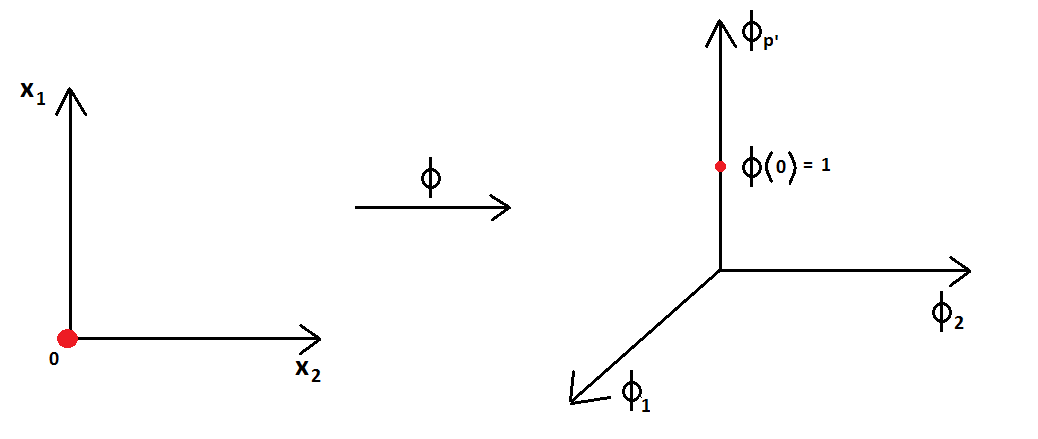
\includegraphics[width=0.9\linewidth]{images/Kernel_nonHomogene}
%\caption{Illustration of samples in $\mathbb{R}^2$. The transformation $\phi$ for a polynomial kernel $K(\textbf{x}_i,\textbf{x}_j)=(\textbf{x}_i^T \textbf{x}_j + c)^d$ with $c=1$ and $d=2$ can be written explicitly: $\phi(\textbf{x}_i)= [x_{i1}^2, x_{i2}^2, \sqrt{2} x_{i1} x_{i2}, 1]^T$. The origin point $\textbf{x}_i=[0,0]^T$ is projected in the Hilbert space as $\phi(\textbf{x}_i=\textbf{0}) = [0, 0, 0, 1]^T$.}
%\label{fig:Kernel_nonHomogene}
%\end{figure}
%
%However, to define proper metrics that respects the properties of metrics (Section \ref{sec:property_metric}), specific kernels must be used. Our work don't propose any solutions to this problem but open the field for new research on this topic. 
%
%
%
%\section{Support Vector Machine (\textsc{svm}) approximation}
%
%
%
%
%\newpage
%\section{Conclusion of the chapter}
%To learn a combined metric $D$ from several unimodal metrics $d_h$ that optimizes the $k$-NN performances, we first proposed a new space representation, the dissimilarity space where each pair of time series is projected as a vector described the unimodal metrics. Then, we propose three formalizations of our metric learning problem: Linear Programming, Quadratic Programming, \textsc{svm}-based approximation. Table \ref{tab:resume_methode} sums up the main pros and cons of each formulation.
%
%\begin{table}[h!]
%	\small
%	\centering
%	\renewcommand{\arraystretch}{0.85}
%	\resizebox{0.6\textwidth}{!}{
%		\setlength{\tabcolsep}{1pt}
%		\begin{tabular}{lccc}
%			\hline
%									& LP	& QP 	& SVM-based\\
%			\hline
%			Linear 					& Yes	& Yes 	& Yes 		\\
%			Non-linear extension 	& No	& Yes 	& Yes 		\\
%			Exact/Approximation resolution	& Exact	& Exact	& Approximation \\
%			Sparcity 				& Yes	& No    & Yes/No 	\\
%			\hline
%		\end{tabular}}
%		\caption{The different formalizations for Metric Learning in Dissimilarity space}
%		\label{tab:resume_methode}
%\end{table}
%  
%In the following, we consider the \textsc{svm}-based approximation because \textsc{svm} framework is well known and well implemented. In the next chapter, we give the details of the steps of our proposed algorithm: Multi-modal and Multi-scale Time series Metric Learning ({\sc m}$^2${\sc tml}).

